\documentclass[twoside]{book}

% Packages required by doxygen
\usepackage{fixltx2e}
\usepackage{calc}
\usepackage{doxygen}
\usepackage[export]{adjustbox} % also loads graphicx
\usepackage{graphicx}
\usepackage[utf8]{inputenc}
\usepackage{makeidx}
\usepackage{multicol}
\usepackage{multirow}
\PassOptionsToPackage{warn}{textcomp}
\usepackage{textcomp}
\usepackage[nointegrals]{wasysym}
\usepackage[table]{xcolor}

% NLS support packages
\usepackage[T2A]{fontenc}
\usepackage[russian]{babel}

% Font selection
\usepackage[T1]{fontenc}
\usepackage[scaled=.90]{helvet}
\usepackage{courier}
\usepackage{amssymb}
\usepackage{sectsty}
\renewcommand{\familydefault}{\sfdefault}
\allsectionsfont{%
  \fontseries{bc}\selectfont%
  \color{darkgray}%
}
\renewcommand{\DoxyLabelFont}{%
  \fontseries{bc}\selectfont%
  \color{darkgray}%
}
\newcommand{\+}{\discretionary{\mbox{\scriptsize$\hookleftarrow$}}{}{}}

% Page & text layout
\usepackage{geometry}
\geometry{%
  a4paper,%
  top=2.5cm,%
  bottom=2.5cm,%
  left=2.5cm,%
  right=2.5cm%
}
\tolerance=750
\hfuzz=15pt
\hbadness=750
\setlength{\emergencystretch}{15pt}
\setlength{\parindent}{0cm}
\setlength{\parskip}{3ex plus 2ex minus 2ex}
\makeatletter
\renewcommand{\paragraph}{%
  \@startsection{paragraph}{4}{0ex}{-1.0ex}{1.0ex}{%
    \normalfont\normalsize\bfseries\SS@parafont%
  }%
}
\renewcommand{\subparagraph}{%
  \@startsection{subparagraph}{5}{0ex}{-1.0ex}{1.0ex}{%
    \normalfont\normalsize\bfseries\SS@subparafont%
  }%
}
\makeatother

% Headers & footers
\usepackage{fancyhdr}
\pagestyle{fancyplain}
\fancyhead[LE]{\fancyplain{}{\bfseries\thepage}}
\fancyhead[CE]{\fancyplain{}{}}
\fancyhead[RE]{\fancyplain{}{\bfseries\leftmark}}
\fancyhead[LO]{\fancyplain{}{\bfseries\rightmark}}
\fancyhead[CO]{\fancyplain{}{}}
\fancyhead[RO]{\fancyplain{}{\bfseries\thepage}}
\fancyfoot[LE]{\fancyplain{}{}}
\fancyfoot[CE]{\fancyplain{}{}}
\fancyfoot[RE]{\fancyplain{}{\bfseries\scriptsize Создано системой Doxygen }}
\fancyfoot[LO]{\fancyplain{}{\bfseries\scriptsize Создано системой Doxygen }}
\fancyfoot[CO]{\fancyplain{}{}}
\fancyfoot[RO]{\fancyplain{}{}}
\renewcommand{\footrulewidth}{0.4pt}
\renewcommand{\chaptermark}[1]{%
  \markboth{#1}{}%
}
\renewcommand{\sectionmark}[1]{%
  \markright{\thesection\ #1}%
}

% Indices & bibliography
\usepackage{natbib}
\usepackage[titles]{tocloft}
\setcounter{tocdepth}{3}
\setcounter{secnumdepth}{5}
\makeindex

% Hyperlinks (required, but should be loaded last)
\usepackage{ifpdf}
\ifpdf
  \usepackage[pdftex,pagebackref=true]{hyperref}
\else
  \usepackage[ps2pdf,pagebackref=true]{hyperref}
\fi
\hypersetup{%
  colorlinks=true,%
  linkcolor=blue,%
  citecolor=blue,%
  unicode%
}

% Custom commands
\newcommand{\clearemptydoublepage}{%
  \newpage{\pagestyle{empty}\cleardoublepage}%
}

\usepackage{caption}
\captionsetup{labelsep=space,justification=centering,font={bf},singlelinecheck=off,skip=4pt,position=top}

%===== C O N T E N T S =====

\begin{document}

% Titlepage & ToC
\hypersetup{pageanchor=false,
             bookmarksnumbered=true,
             pdfencoding=unicode
            }
\pagenumbering{alph}
\begin{titlepage}
\vspace*{7cm}
\begin{center}%
{\Large Программа по телемедицине \\[1ex]\large 1.\+0 }\\
\vspace*{1cm}
{\large Создано системой Doxygen 1.8.13}\\
\end{center}
\end{titlepage}
\clearemptydoublepage
\pagenumbering{roman}
\tableofcontents
\clearemptydoublepage
\pagenumbering{arabic}
\hypersetup{pageanchor=true}

%--- Begin generated contents ---
\chapter{Список задач}
\label{todo}
\Hypertarget{todo}

\begin{DoxyRefList}
\item[\label{todo__todo000001}%
\Hypertarget{todo__todo000001}%
Класс \hyperlink{classAccessibilityForm}{Accessibility\+Form} ]Запись в базу объекта ответа
\end{DoxyRefList}
\chapter{Алфавитный указатель пространств имен}
\section{Пространства имен}
Полный список пространств имен.\begin{DoxyCompactList}
\item\contentsline{section}{\hyperlink{namespaceSerialize}{Serialize} }{\pageref{namespaceSerialize}}{}
\item\contentsline{section}{\hyperlink{namespacetableFields}{table\+Fields} }{\pageref{namespacetableFields}}{}
\item\contentsline{section}{\hyperlink{namespaceUi}{Ui} }{\pageref{namespaceUi}}{}
\end{DoxyCompactList}

\chapter{Иерархический список классов}
\section{Иерархия классов}
Иерархия классов.\begin{DoxyCompactList}
\item Q\+Dialog\begin{DoxyCompactList}
\item \contentsline{section}{Send\+Dialog}{\pageref{classSendDialog}}{}
\end{DoxyCompactList}
\item Q\+Exception\begin{DoxyCompactList}
\item \contentsline{section}{Tele\+Med\+Obj\+Exception}{\pageref{classTeleMedObjException}}{}
\end{DoxyCompactList}
\item Q\+Graphics\+View\begin{DoxyCompactList}
\item \contentsline{section}{Scene\+Zoom}{\pageref{classSceneZoom}}{}
\end{DoxyCompactList}
\item Q\+Main\+Window\begin{DoxyCompactList}
\item \contentsline{section}{Main\+Window}{\pageref{classMainWindow}}{}
\end{DoxyCompactList}
\item Q\+Object\begin{DoxyCompactList}
\item \contentsline{section}{Client}{\pageref{classClient}}{}
\item \contentsline{section}{Task}{\pageref{classTask}}{}
\end{DoxyCompactList}
\item Q\+Runnable\begin{DoxyCompactList}
\item \contentsline{section}{Task}{\pageref{classTask}}{}
\end{DoxyCompactList}
\item Q\+Tcp\+Server\begin{DoxyCompactList}
\item \contentsline{section}{Server}{\pageref{classServer}}{}
\end{DoxyCompactList}
\item Q\+Widget\begin{DoxyCompactList}
\item \contentsline{section}{Accessibility\+Form}{\pageref{classAccessibilityForm}}{}
\item \contentsline{section}{Db\+Form}{\pageref{classDbForm}}{}
\item \contentsline{section}{Side\+Bar}{\pageref{classSideBar}}{}
\item \contentsline{section}{Viewer\+Form}{\pageref{classViewerForm}}{}
\end{DoxyCompactList}
\item \contentsline{section}{Tele\+Med\+Object}{\pageref{classTeleMedObject}}{}
\end{DoxyCompactList}

\chapter{Алфавитный указатель классов}
\section{Классы}
Классы с их кратким описанием.\begin{DoxyCompactList}
\item\contentsline{section}{\hyperlink{classAccessibilityForm}{Accessibility\+Form} \\*Класс формы для осуществления сетевого взаимодействия }{\pageref{classAccessibilityForm}}{}
\item\contentsline{section}{\hyperlink{classClient}{Client} \\*Класс имитирующий клиента подключенного к серверу }{\pageref{classClient}}{}
\item\contentsline{section}{\hyperlink{classDbForm}{Db\+Form} \\*Класс формы для отображения содержимого базы данных }{\pageref{classDbForm}}{}
\item\contentsline{section}{\hyperlink{classMainWindow}{Main\+Window} \\*Класс главного окна программы }{\pageref{classMainWindow}}{}
\item\contentsline{section}{\hyperlink{classSceneZoom}{Scene\+Zoom} \\*Класс реализующий логику зумирования изображения в сцене на виджете }{\pageref{classSceneZoom}}{}
\item\contentsline{section}{\hyperlink{classSendDialog}{Send\+Dialog} \\*Класс формы отправки запроса }{\pageref{classSendDialog}}{}
\item\contentsline{section}{\hyperlink{classServer}{Server} \\*Класс сервера }{\pageref{classServer}}{}
\item\contentsline{section}{\hyperlink{classSideBar}{Side\+Bar} \\*Класс формы боковой панели выбора виджета }{\pageref{classSideBar}}{}
\item\contentsline{section}{\hyperlink{classTask}{Task} \\*Класс задачи }{\pageref{classTask}}{}
\item\contentsline{section}{\hyperlink{classTeleMedObject}{Tele\+Med\+Object} \\*Класс объекта информации в телемедицинском сеансе }{\pageref{classTeleMedObject}}{}
\item\contentsline{section}{\hyperlink{classTeleMedObjException}{Tele\+Med\+Obj\+Exception} \\*Класс исключения при построении объекта информации }{\pageref{classTeleMedObjException}}{}
\item\contentsline{section}{\hyperlink{classViewerForm}{Viewer\+Form} \\*Класс формы для отображения файлов dcm }{\pageref{classViewerForm}}{}
\end{DoxyCompactList}

\chapter{Список файлов}
\section{Файлы}
Полный список файлов.\begin{DoxyCompactList}
\item\contentsline{section}{\hyperlink{accessibilityform_8cpp}{accessibilityform.\+cpp} }{\pageref{accessibilityform_8cpp}}{}
\item\contentsline{section}{\hyperlink{accessibilityform_8h}{accessibilityform.\+h} }{\pageref{accessibilityform_8h}}{}
\item\contentsline{section}{\hyperlink{client_8cpp}{client.\+cpp} }{\pageref{client_8cpp}}{}
\item\contentsline{section}{\hyperlink{client_8h}{client.\+h} }{\pageref{client_8h}}{}
\item\contentsline{section}{\hyperlink{converters_8cpp}{converters.\+cpp} }{\pageref{converters_8cpp}}{}
\item\contentsline{section}{\hyperlink{converters_8h}{converters.\+h} }{\pageref{converters_8h}}{}
\item\contentsline{section}{\hyperlink{dbform_8cpp}{dbform.\+cpp} }{\pageref{dbform_8cpp}}{}
\item\contentsline{section}{\hyperlink{dbform_8h}{dbform.\+h} }{\pageref{dbform_8h}}{}
\item\contentsline{section}{\hyperlink{logger_8cpp}{logger.\+cpp} }{\pageref{logger_8cpp}}{}
\item\contentsline{section}{\hyperlink{logger_8h}{logger.\+h} }{\pageref{logger_8h}}{}
\item\contentsline{section}{\hyperlink{main_8cpp}{main.\+cpp} }{\pageref{main_8cpp}}{}
\item\contentsline{section}{\hyperlink{mainwindow_8cpp}{mainwindow.\+cpp} }{\pageref{mainwindow_8cpp}}{}
\item\contentsline{section}{\hyperlink{mainwindow_8h}{mainwindow.\+h} }{\pageref{mainwindow_8h}}{}
\item\contentsline{section}{\hyperlink{scenezoom_8cpp}{scenezoom.\+cpp} }{\pageref{scenezoom_8cpp}}{}
\item\contentsline{section}{\hyperlink{scenezoom_8h}{scenezoom.\+h} }{\pageref{scenezoom_8h}}{}
\item\contentsline{section}{\hyperlink{senddialog_8cpp}{senddialog.\+cpp} }{\pageref{senddialog_8cpp}}{}
\item\contentsline{section}{\hyperlink{senddialog_8h}{senddialog.\+h} }{\pageref{senddialog_8h}}{}
\item\contentsline{section}{\hyperlink{serializehelper_8cpp}{serializehelper.\+cpp} }{\pageref{serializehelper_8cpp}}{}
\item\contentsline{section}{\hyperlink{serializehelper_8h}{serializehelper.\+h} }{\pageref{serializehelper_8h}}{}
\item\contentsline{section}{\hyperlink{server_8cpp}{server.\+cpp} }{\pageref{server_8cpp}}{}
\item\contentsline{section}{\hyperlink{server_8h}{server.\+h} }{\pageref{server_8h}}{}
\item\contentsline{section}{\hyperlink{sidebar_8cpp}{sidebar.\+cpp} }{\pageref{sidebar_8cpp}}{}
\item\contentsline{section}{\hyperlink{sidebar_8h}{sidebar.\+h} }{\pageref{sidebar_8h}}{}
\item\contentsline{section}{\hyperlink{tablefields_8h}{tablefields.\+h} }{\pageref{tablefields_8h}}{}
\item\contentsline{section}{\hyperlink{tagshelpers_8cpp}{tagshelpers.\+cpp} }{\pageref{tagshelpers_8cpp}}{}
\item\contentsline{section}{\hyperlink{tagshelpers_8h}{tagshelpers.\+h} }{\pageref{tagshelpers_8h}}{}
\item\contentsline{section}{\hyperlink{task_8cpp}{task.\+cpp} }{\pageref{task_8cpp}}{}
\item\contentsline{section}{\hyperlink{task_8h}{task.\+h} }{\pageref{task_8h}}{}
\item\contentsline{section}{\hyperlink{telemedobject_8cpp}{telemedobject.\+cpp} }{\pageref{telemedobject_8cpp}}{}
\item\contentsline{section}{\hyperlink{telemedobject_8h}{telemedobject.\+h} }{\pageref{telemedobject_8h}}{}
\item\contentsline{section}{\hyperlink{viewerform_8cpp}{viewerform.\+cpp} }{\pageref{viewerform_8cpp}}{}
\item\contentsline{section}{\hyperlink{viewerform_8h}{viewerform.\+h} }{\pageref{viewerform_8h}}{}
\end{DoxyCompactList}

\chapter{Пространства имен}
\hypertarget{namespaceSerialize}{}\section{Пространство имен Serialize}
\label{namespaceSerialize}\index{Serialize@{Serialize}}
\subsection*{Функции}
\begin{DoxyCompactItemize}
\item 
Q\+Byte\+Array \hyperlink{namespaceSerialize_a11412877176c667f31a331bfac95d7e1}{image\+To\+Byte\+Array} (const Q\+Image \&image)
\begin{DoxyCompactList}\small\item\em image\+To\+Byte\+Array \end{DoxyCompactList}\item 
Q\+Image \hyperlink{namespaceSerialize_ad70935346b9a0522990d0ff87e963a26}{byte\+Array\+To\+Image} (const Q\+Byte\+Array \&ba)
\begin{DoxyCompactList}\small\item\em byte\+Array\+To\+Image \end{DoxyCompactList}\item 
Q\+Json\+Value \hyperlink{namespaceSerialize_a794b837e3f9323b238c5b4d115f5c78b}{json\+Val\+From\+Image} (const Q\+Image \&p)
\begin{DoxyCompactList}\small\item\em json\+Val\+From\+Image \end{DoxyCompactList}\item 
Q\+Image \hyperlink{namespaceSerialize_a966ed9963741cb19a07f8b057faae920}{image\+From} (const Q\+Json\+Value \&val)
\begin{DoxyCompactList}\small\item\em image\+From \end{DoxyCompactList}\item 
{\footnotesize template$<$class T $>$ }\\auto \hyperlink{namespaceSerialize_a5318048e43f2cacc610f177d093283f8}{dict\+To\+Byte\+Array} (const T \&dict) -\/$>$ Q\+Byte\+Array
\begin{DoxyCompactList}\small\item\em dict\+To\+Byte\+Array \end{DoxyCompactList}\item 
{\footnotesize template$<$class T $>$ }\\T \hyperlink{namespaceSerialize_aac818c4b807e223e916bbe829e0d86ea}{byte\+Array\+To\+Dict} (Q\+Byte\+Array $\ast$ba)
\begin{DoxyCompactList}\small\item\em byte\+Array\+To\+Dict \end{DoxyCompactList}\item 
{\footnotesize template$<$class T $>$ }\\T \hyperlink{namespaceSerialize_ac2bf64c91d863df6a6c6149c7a482af0}{dict\+From\+Base64} (const Q\+Json\+Value \&value)
\begin{DoxyCompactList}\small\item\em dict\+From\+Base64 \end{DoxyCompactList}\end{DoxyCompactItemize}


\subsection{Функции}
\mbox{\Hypertarget{namespaceSerialize_aac818c4b807e223e916bbe829e0d86ea}\label{namespaceSerialize_aac818c4b807e223e916bbe829e0d86ea}} 
\index{Serialize@{Serialize}!byte\+Array\+To\+Dict@{byte\+Array\+To\+Dict}}
\index{byte\+Array\+To\+Dict@{byte\+Array\+To\+Dict}!Serialize@{Serialize}}
\subsubsection{\texorpdfstring{byte\+Array\+To\+Dict()}{byteArrayToDict()}}
{\footnotesize\ttfamily template$<$class T $>$ \\
T Serialize\+::byte\+Array\+To\+Dict (\begin{DoxyParamCaption}\item[{Q\+Byte\+Array $\ast$}]{ba }\end{DoxyParamCaption})}



byte\+Array\+To\+Dict 

Шаблон для сериализации бинарных данных в словарь \mbox{\Hypertarget{namespaceSerialize_ad70935346b9a0522990d0ff87e963a26}\label{namespaceSerialize_ad70935346b9a0522990d0ff87e963a26}} 
\index{Serialize@{Serialize}!byte\+Array\+To\+Image@{byte\+Array\+To\+Image}}
\index{byte\+Array\+To\+Image@{byte\+Array\+To\+Image}!Serialize@{Serialize}}
\subsubsection{\texorpdfstring{byte\+Array\+To\+Image()}{byteArrayToImage()}}
{\footnotesize\ttfamily Q\+Image Serialize\+::byte\+Array\+To\+Image (\begin{DoxyParamCaption}\item[{const Q\+Byte\+Array \&}]{ba }\end{DoxyParamCaption})}



byte\+Array\+To\+Image 


\begin{DoxyParams}{Аргументы}
{\em ba} & Набор байт \\
\hline
\end{DoxyParams}
\begin{DoxyReturn}{Возвращает}
Изображение
\end{DoxyReturn}
Функция конвертирует бинарные данные в изображение \mbox{\Hypertarget{namespaceSerialize_ac2bf64c91d863df6a6c6149c7a482af0}\label{namespaceSerialize_ac2bf64c91d863df6a6c6149c7a482af0}} 
\index{Serialize@{Serialize}!dict\+From\+Base64@{dict\+From\+Base64}}
\index{dict\+From\+Base64@{dict\+From\+Base64}!Serialize@{Serialize}}
\subsubsection{\texorpdfstring{dict\+From\+Base64()}{dictFromBase64()}}
{\footnotesize\ttfamily template$<$class T $>$ \\
T Serialize\+::dict\+From\+Base64 (\begin{DoxyParamCaption}\item[{const Q\+Json\+Value \&}]{value }\end{DoxyParamCaption})}



dict\+From\+Base64 

Шаблон для сериализации бинарных данных в кодировке basе64 в словарь \mbox{\Hypertarget{namespaceSerialize_a5318048e43f2cacc610f177d093283f8}\label{namespaceSerialize_a5318048e43f2cacc610f177d093283f8}} 
\index{Serialize@{Serialize}!dict\+To\+Byte\+Array@{dict\+To\+Byte\+Array}}
\index{dict\+To\+Byte\+Array@{dict\+To\+Byte\+Array}!Serialize@{Serialize}}
\subsubsection{\texorpdfstring{dict\+To\+Byte\+Array()}{dictToByteArray()}}
{\footnotesize\ttfamily template$<$class T $>$ \\
auto Serialize\+::dict\+To\+Byte\+Array (\begin{DoxyParamCaption}\item[{const T \&}]{dict }\end{DoxyParamCaption}) -\/$>$ Q\+Byte\+Array}



dict\+To\+Byte\+Array 

Шаблон для сериализации типа словарь в бинарные данные \mbox{\Hypertarget{namespaceSerialize_a966ed9963741cb19a07f8b057faae920}\label{namespaceSerialize_a966ed9963741cb19a07f8b057faae920}} 
\index{Serialize@{Serialize}!image\+From@{image\+From}}
\index{image\+From@{image\+From}!Serialize@{Serialize}}
\subsubsection{\texorpdfstring{image\+From()}{imageFrom()}}
{\footnotesize\ttfamily Q\+Image Serialize\+::image\+From (\begin{DoxyParamCaption}\item[{const Q\+Json\+Value \&}]{val }\end{DoxyParamCaption})}



image\+From 


\begin{DoxyParams}{Аргументы}
{\em val} & Ключ -\/ значение с изображение \\
\hline
\end{DoxyParams}
\begin{DoxyReturn}{Возвращает}
Объект изображения
\end{DoxyReturn}
Функция тип ключ значение, где ключ -\/ image, значение -\/ бинарные данные в объект изображения \mbox{\Hypertarget{namespaceSerialize_a11412877176c667f31a331bfac95d7e1}\label{namespaceSerialize_a11412877176c667f31a331bfac95d7e1}} 
\index{Serialize@{Serialize}!image\+To\+Byte\+Array@{image\+To\+Byte\+Array}}
\index{image\+To\+Byte\+Array@{image\+To\+Byte\+Array}!Serialize@{Serialize}}
\subsubsection{\texorpdfstring{image\+To\+Byte\+Array()}{imageToByteArray()}}
{\footnotesize\ttfamily Q\+Byte\+Array Serialize\+::image\+To\+Byte\+Array (\begin{DoxyParamCaption}\item[{const Q\+Image \&}]{image }\end{DoxyParamCaption})}



image\+To\+Byte\+Array 


\begin{DoxyParams}{Аргументы}
{\em image} & Изображение \\
\hline
\end{DoxyParams}
\begin{DoxyReturn}{Возвращает}
Набор байт
\end{DoxyReturn}
Функция сериализует объект изображения в бинарные данные \mbox{\Hypertarget{namespaceSerialize_a794b837e3f9323b238c5b4d115f5c78b}\label{namespaceSerialize_a794b837e3f9323b238c5b4d115f5c78b}} 
\index{Serialize@{Serialize}!json\+Val\+From\+Image@{json\+Val\+From\+Image}}
\index{json\+Val\+From\+Image@{json\+Val\+From\+Image}!Serialize@{Serialize}}
\subsubsection{\texorpdfstring{json\+Val\+From\+Image()}{jsonValFromImage()}}
{\footnotesize\ttfamily Q\+Json\+Value Serialize\+::json\+Val\+From\+Image (\begin{DoxyParamCaption}\item[{const Q\+Image \&}]{p }\end{DoxyParamCaption})}



json\+Val\+From\+Image 


\begin{DoxyParams}{Аргументы}
{\em p} & Изображение \\
\hline
\end{DoxyParams}
\begin{DoxyReturn}{Возвращает}
Объект типа ключ в структуре json
\end{DoxyReturn}
Функция конвертирует изображение в тип ключ значение, где ключ -\/ image, значение -\/ бинарные данные 
\hypertarget{namespacetableFields}{}\section{Пространство имен table\+Fields}
\label{namespacetableFields}\index{table\+Fields@{table\+Fields}}
\subsection*{Перечисления}
\begin{DoxyCompactItemize}
\item 
enum \hyperlink{namespacetableFields_af3f3b90a55c2fc0e89652786698aff33}{table\+Fields} \{ \newline
\hyperlink{namespacetableFields_af3f3b90a55c2fc0e89652786698aff33a3688697bcb72b96772a0b8bba66cf1f7}{table\+\_\+id} = 0, 
\hyperlink{namespacetableFields_af3f3b90a55c2fc0e89652786698aff33aac6d4c2d5e73ed2e112948441fa690f2}{table\+\_\+name} = 1, 
\hyperlink{namespacetableFields_af3f3b90a55c2fc0e89652786698aff33a0fbe15558786dbadd11790fa61e16cda}{table\+\_\+image} = 2, 
\hyperlink{namespacetableFields_af3f3b90a55c2fc0e89652786698aff33a4699aeeba4e2c1b5addebc6fde4e004e}{table\+\_\+data} = 3, 
\newline
\hyperlink{namespacetableFields_af3f3b90a55c2fc0e89652786698aff33a69b6cda96cbc1bd9d9fed0c8a0446d14}{table\+\_\+request} = 4, 
\hyperlink{namespacetableFields_af3f3b90a55c2fc0e89652786698aff33a7d5985177bdc214aa76c2956da19b292}{table\+\_\+response} = 5, 
\hyperlink{namespacetableFields_af3f3b90a55c2fc0e89652786698aff33a2488fe0a3fd10b94548a37839474f12a}{table\+\_\+request\+\_\+date} = 6, 
\hyperlink{namespacetableFields_af3f3b90a55c2fc0e89652786698aff33a08521c2e57d6cd782177ff9410c234a7}{table\+\_\+response\+\_\+date} = 7, 
\newline
\hyperlink{namespacetableFields_af3f3b90a55c2fc0e89652786698aff33af6c67a88169df220165a3f4b3edc5ca7}{table\+\_\+requester} = 8, 
\hyperlink{namespacetableFields_af3f3b90a55c2fc0e89652786698aff33abd83777ee433cf1acf2c16b45f03e677}{table\+\_\+responser} = 9
 \}
\end{DoxyCompactItemize}


\subsection{Подробное описание}
Структура для отображения числовых значений колонок в таблице базы данных на смысловое значение информации в этих колонках 

\subsection{Перечисления}
\mbox{\Hypertarget{namespacetableFields_af3f3b90a55c2fc0e89652786698aff33}\label{namespacetableFields_af3f3b90a55c2fc0e89652786698aff33}} 
\index{table\+Fields@{table\+Fields}!table\+Fields@{table\+Fields}}
\index{table\+Fields@{table\+Fields}!table\+Fields@{table\+Fields}}
\subsubsection{\texorpdfstring{table\+Fields}{tableFields}}
{\footnotesize\ttfamily enum \hyperlink{namespacetableFields_af3f3b90a55c2fc0e89652786698aff33}{table\+Fields\+::table\+Fields}}

\begin{DoxyEnumFields}{Элементы перечислений}
\raisebox{\heightof{T}}[0pt][0pt]{\index{table\+\_\+id@{table\+\_\+id}!table\+Fields@{table\+Fields}}\index{table\+Fields@{table\+Fields}!table\+\_\+id@{table\+\_\+id}}}\mbox{\Hypertarget{namespacetableFields_af3f3b90a55c2fc0e89652786698aff33a3688697bcb72b96772a0b8bba66cf1f7}\label{namespacetableFields_af3f3b90a55c2fc0e89652786698aff33a3688697bcb72b96772a0b8bba66cf1f7}} 
table\+\_\+id&\\
\hline

\raisebox{\heightof{T}}[0pt][0pt]{\index{table\+\_\+name@{table\+\_\+name}!table\+Fields@{table\+Fields}}\index{table\+Fields@{table\+Fields}!table\+\_\+name@{table\+\_\+name}}}\mbox{\Hypertarget{namespacetableFields_af3f3b90a55c2fc0e89652786698aff33aac6d4c2d5e73ed2e112948441fa690f2}\label{namespacetableFields_af3f3b90a55c2fc0e89652786698aff33aac6d4c2d5e73ed2e112948441fa690f2}} 
table\+\_\+name&\\
\hline

\raisebox{\heightof{T}}[0pt][0pt]{\index{table\+\_\+image@{table\+\_\+image}!table\+Fields@{table\+Fields}}\index{table\+Fields@{table\+Fields}!table\+\_\+image@{table\+\_\+image}}}\mbox{\Hypertarget{namespacetableFields_af3f3b90a55c2fc0e89652786698aff33a0fbe15558786dbadd11790fa61e16cda}\label{namespacetableFields_af3f3b90a55c2fc0e89652786698aff33a0fbe15558786dbadd11790fa61e16cda}} 
table\+\_\+image&\\
\hline

\raisebox{\heightof{T}}[0pt][0pt]{\index{table\+\_\+data@{table\+\_\+data}!table\+Fields@{table\+Fields}}\index{table\+Fields@{table\+Fields}!table\+\_\+data@{table\+\_\+data}}}\mbox{\Hypertarget{namespacetableFields_af3f3b90a55c2fc0e89652786698aff33a4699aeeba4e2c1b5addebc6fde4e004e}\label{namespacetableFields_af3f3b90a55c2fc0e89652786698aff33a4699aeeba4e2c1b5addebc6fde4e004e}} 
table\+\_\+data&\\
\hline

\raisebox{\heightof{T}}[0pt][0pt]{\index{table\+\_\+request@{table\+\_\+request}!table\+Fields@{table\+Fields}}\index{table\+Fields@{table\+Fields}!table\+\_\+request@{table\+\_\+request}}}\mbox{\Hypertarget{namespacetableFields_af3f3b90a55c2fc0e89652786698aff33a69b6cda96cbc1bd9d9fed0c8a0446d14}\label{namespacetableFields_af3f3b90a55c2fc0e89652786698aff33a69b6cda96cbc1bd9d9fed0c8a0446d14}} 
table\+\_\+request&\\
\hline

\raisebox{\heightof{T}}[0pt][0pt]{\index{table\+\_\+response@{table\+\_\+response}!table\+Fields@{table\+Fields}}\index{table\+Fields@{table\+Fields}!table\+\_\+response@{table\+\_\+response}}}\mbox{\Hypertarget{namespacetableFields_af3f3b90a55c2fc0e89652786698aff33a7d5985177bdc214aa76c2956da19b292}\label{namespacetableFields_af3f3b90a55c2fc0e89652786698aff33a7d5985177bdc214aa76c2956da19b292}} 
table\+\_\+response&\\
\hline

\raisebox{\heightof{T}}[0pt][0pt]{\index{table\+\_\+request\+\_\+date@{table\+\_\+request\+\_\+date}!table\+Fields@{table\+Fields}}\index{table\+Fields@{table\+Fields}!table\+\_\+request\+\_\+date@{table\+\_\+request\+\_\+date}}}\mbox{\Hypertarget{namespacetableFields_af3f3b90a55c2fc0e89652786698aff33a2488fe0a3fd10b94548a37839474f12a}\label{namespacetableFields_af3f3b90a55c2fc0e89652786698aff33a2488fe0a3fd10b94548a37839474f12a}} 
table\+\_\+request\+\_\+date&\\
\hline

\raisebox{\heightof{T}}[0pt][0pt]{\index{table\+\_\+response\+\_\+date@{table\+\_\+response\+\_\+date}!table\+Fields@{table\+Fields}}\index{table\+Fields@{table\+Fields}!table\+\_\+response\+\_\+date@{table\+\_\+response\+\_\+date}}}\mbox{\Hypertarget{namespacetableFields_af3f3b90a55c2fc0e89652786698aff33a08521c2e57d6cd782177ff9410c234a7}\label{namespacetableFields_af3f3b90a55c2fc0e89652786698aff33a08521c2e57d6cd782177ff9410c234a7}} 
table\+\_\+response\+\_\+date&\\
\hline

\raisebox{\heightof{T}}[0pt][0pt]{\index{table\+\_\+requester@{table\+\_\+requester}!table\+Fields@{table\+Fields}}\index{table\+Fields@{table\+Fields}!table\+\_\+requester@{table\+\_\+requester}}}\mbox{\Hypertarget{namespacetableFields_af3f3b90a55c2fc0e89652786698aff33af6c67a88169df220165a3f4b3edc5ca7}\label{namespacetableFields_af3f3b90a55c2fc0e89652786698aff33af6c67a88169df220165a3f4b3edc5ca7}} 
table\+\_\+requester&\\
\hline

\raisebox{\heightof{T}}[0pt][0pt]{\index{table\+\_\+responser@{table\+\_\+responser}!table\+Fields@{table\+Fields}}\index{table\+Fields@{table\+Fields}!table\+\_\+responser@{table\+\_\+responser}}}\mbox{\Hypertarget{namespacetableFields_af3f3b90a55c2fc0e89652786698aff33abd83777ee433cf1acf2c16b45f03e677}\label{namespacetableFields_af3f3b90a55c2fc0e89652786698aff33abd83777ee433cf1acf2c16b45f03e677}} 
table\+\_\+responser&\\
\hline

\end{DoxyEnumFields}

\hypertarget{namespaceUi}{}\section{Пространство имен Ui}
\label{namespaceUi}\index{Ui@{Ui}}

\chapter{Классы}
\hypertarget{classAccessibilityForm}{}\section{Класс Accessibility\+Form}
\label{classAccessibilityForm}\index{Accessibility\+Form@{Accessibility\+Form}}


Класс формы для осуществления сетевого взаимодействия.  




{\ttfamily \#include $<$accessibilityform.\+h$>$}



Граф наследования\+:Accessibility\+Form\+:\nopagebreak
\begin{figure}[H]
\begin{center}
\leavevmode
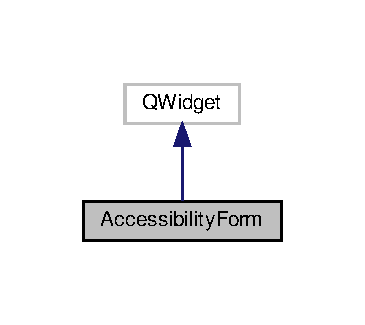
\includegraphics[width=175pt]{classAccessibilityForm__inherit__graph}
\end{center}
\end{figure}


Граф связей класса Accessibility\+Form\+:
\nopagebreak
\begin{figure}[H]
\begin{center}
\leavevmode
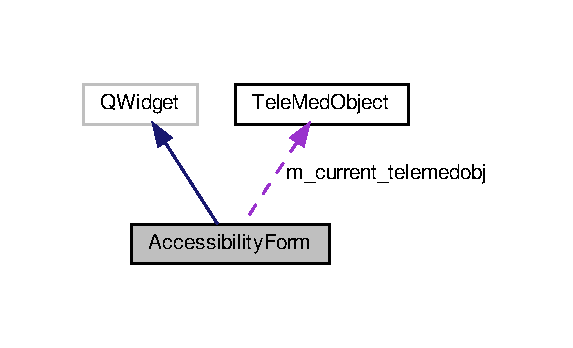
\includegraphics[width=275pt]{classAccessibilityForm__coll__graph}
\end{center}
\end{figure}
\subsection*{Открытые слоты}
\begin{DoxyCompactItemize}
\item 
void \hyperlink{classAccessibilityForm_a0c75d12469be97cc2e80a2a7e5db66d5}{get\+Data\+From\+Server} (Q\+Byte\+Array ba)
\begin{DoxyCompactList}\small\item\em get\+Data\+From\+Server \end{DoxyCompactList}\end{DoxyCompactItemize}
\subsection*{Сигналы}
\begin{DoxyCompactItemize}
\item 
void \hyperlink{classAccessibilityForm_abd079103500734db443b13a5f177938c}{send\+Signal\+To\+Dump} (Q\+String \&name, Q\+Image \&image, \hyperlink{tagshelpers_8h_ae25d30658f61420b88a380dc9e40bb74}{dicom\+Dict} \&dict, \hyperlink{dbform_8h_a1ec1a645f41e1c6544d384ca863a936c}{add\+Info\+Map} \&map)
\begin{DoxyCompactList}\small\item\em send\+Signal\+To\+Dump \end{DoxyCompactList}\end{DoxyCompactItemize}
\subsection*{Открытые члены}
\begin{DoxyCompactItemize}
\item 
\hyperlink{classAccessibilityForm_aed3d56ba8bea5e204065b33aeabc501f}{Accessibility\+Form} (Q\+Widget $\ast$parent=nullptr)
\begin{DoxyCompactList}\small\item\em \hyperlink{classAccessibilityForm}{Accessibility\+Form}. \end{DoxyCompactList}\item 
bool \hyperlink{classAccessibilityForm_a8c465f42556cfec6742dc973e8f3580b}{ask\+For\+Save} ()
\begin{DoxyCompactList}\small\item\em ask\+For\+Save \end{DoxyCompactList}\item 
\hyperlink{classAccessibilityForm_a35c94d7857e2a4db9a8fe5c60ecc8e64}{$\sim$\+Accessibility\+Form} ()
\end{DoxyCompactItemize}
\subsection*{Открытые атрибуты}
\begin{DoxyCompactItemize}
\item 
Q\+Graphics\+Scene $\ast$ \hyperlink{classAccessibilityForm_a5ce983d3b40e1486857d263b11fda575}{scene}
\end{DoxyCompactItemize}
\subsection*{Закрытые слоты}
\begin{DoxyCompactItemize}
\item 
void \hyperlink{classAccessibilityForm_a47e343e6d2668e2fb9d79c3a4e342bfd}{on\+\_\+request\+Button\+\_\+clicked} ()
\begin{DoxyCompactList}\small\item\em on\+\_\+request\+Button\+\_\+clicked \end{DoxyCompactList}\item 
void \hyperlink{classAccessibilityForm_aa9ec98dd84724349a77477f0431298dc}{on\+\_\+response\+Button\+\_\+clicked} ()
\begin{DoxyCompactList}\small\item\em on\+\_\+response\+Button\+\_\+clicked \end{DoxyCompactList}\end{DoxyCompactItemize}
\subsection*{Закрытые члены}
\begin{DoxyCompactItemize}
\item 
void \hyperlink{classAccessibilityForm_adc4f7fd9320458525471566366e33030}{show\+Current\+Obj} ()
\begin{DoxyCompactList}\small\item\em show\+Current\+Obj \end{DoxyCompactList}\end{DoxyCompactItemize}
\subsection*{Закрытые данные}
\begin{DoxyCompactItemize}
\item 
\hyperlink{classTeleMedObject}{Tele\+Med\+Object} \hyperlink{classAccessibilityForm_a7abf8a65145b6a1164e15fe5667156ab}{m\+\_\+current\+\_\+telemedobj}
\begin{DoxyCompactList}\small\item\em m\+\_\+current\+\_\+telemedobj \end{DoxyCompactList}\item 
Ui\+::\+Accessibility\+Form $\ast$ \hyperlink{classAccessibilityForm_a410e78e46d46b2e5785277eba28fc8de}{ui}
\begin{DoxyCompactList}\small\item\em ui \end{DoxyCompactList}\end{DoxyCompactItemize}


\subsection{Подробное описание}
Класс формы для осуществления сетевого взаимодействия. 

\begin{DoxyAuthor}{Автор}
Илья Трефилов 
\end{DoxyAuthor}
\begin{DoxyDate}{Дата}
01.\+12.\+2018 
\end{DoxyDate}
\begin{DoxyRefDesc}{Необходимо сделать}
\item[\hyperlink{todo__todo000001}{Необходимо сделать}]Запись в базу объекта ответа\end{DoxyRefDesc}


Данный класс предназначен для управления функциями, виджета \char`\"{}Сетевое взаимодействие\char`\"{} 

\subsection{Конструктор(ы)}
\mbox{\Hypertarget{classAccessibilityForm_aed3d56ba8bea5e204065b33aeabc501f}\label{classAccessibilityForm_aed3d56ba8bea5e204065b33aeabc501f}} 
\index{Accessibility\+Form@{Accessibility\+Form}!Accessibility\+Form@{Accessibility\+Form}}
\index{Accessibility\+Form@{Accessibility\+Form}!Accessibility\+Form@{Accessibility\+Form}}
\subsubsection{\texorpdfstring{Accessibility\+Form()}{AccessibilityForm()}}
{\footnotesize\ttfamily Accessibility\+Form\+::\+Accessibility\+Form (\begin{DoxyParamCaption}\item[{Q\+Widget $\ast$}]{parent = {\ttfamily nullptr} }\end{DoxyParamCaption})\hspace{0.3cm}{\ttfamily [explicit]}}



\hyperlink{classAccessibilityForm}{Accessibility\+Form}. 


\begin{DoxyParams}{Аргументы}
{\em parent} & Конструтор класса, принимающий в параметре ссылку на родительский виджет \\
\hline
\end{DoxyParams}
\mbox{\Hypertarget{classAccessibilityForm_a35c94d7857e2a4db9a8fe5c60ecc8e64}\label{classAccessibilityForm_a35c94d7857e2a4db9a8fe5c60ecc8e64}} 
\index{Accessibility\+Form@{Accessibility\+Form}!````~Accessibility\+Form@{$\sim$\+Accessibility\+Form}}
\index{````~Accessibility\+Form@{$\sim$\+Accessibility\+Form}!Accessibility\+Form@{Accessibility\+Form}}
\subsubsection{\texorpdfstring{$\sim$\+Accessibility\+Form()}{~AccessibilityForm()}}
{\footnotesize\ttfamily Accessibility\+Form\+::$\sim$\+Accessibility\+Form (\begin{DoxyParamCaption}{ }\end{DoxyParamCaption})}



\subsection{Методы}
\mbox{\Hypertarget{classAccessibilityForm_a8c465f42556cfec6742dc973e8f3580b}\label{classAccessibilityForm_a8c465f42556cfec6742dc973e8f3580b}} 
\index{Accessibility\+Form@{Accessibility\+Form}!ask\+For\+Save@{ask\+For\+Save}}
\index{ask\+For\+Save@{ask\+For\+Save}!Accessibility\+Form@{Accessibility\+Form}}
\subsubsection{\texorpdfstring{ask\+For\+Save()}{askForSave()}}
{\footnotesize\ttfamily bool Accessibility\+Form\+::ask\+For\+Save (\begin{DoxyParamCaption}{ }\end{DoxyParamCaption})}



ask\+For\+Save 

\begin{DoxyReturn}{Возвращает}
Возвращает значение типа boolean, указывающее на необходимость сохранения в базу данных
\end{DoxyReturn}
Если функция вернула true -\/ посылаем сигнал сохранения в базу данных \mbox{\Hypertarget{classAccessibilityForm_a0c75d12469be97cc2e80a2a7e5db66d5}\label{classAccessibilityForm_a0c75d12469be97cc2e80a2a7e5db66d5}} 
\index{Accessibility\+Form@{Accessibility\+Form}!get\+Data\+From\+Server@{get\+Data\+From\+Server}}
\index{get\+Data\+From\+Server@{get\+Data\+From\+Server}!Accessibility\+Form@{Accessibility\+Form}}
\subsubsection{\texorpdfstring{get\+Data\+From\+Server}{getDataFromServer}}
{\footnotesize\ttfamily void Accessibility\+Form\+::get\+Data\+From\+Server (\begin{DoxyParamCaption}\item[{Q\+Byte\+Array}]{ba }\end{DoxyParamCaption})\hspace{0.3cm}{\ttfamily [slot]}}



get\+Data\+From\+Server 


\begin{DoxyParams}{Аргументы}
{\em ba} & Набор байт, сформированный при отправке сообщения\\
\hline
\end{DoxyParams}
Функция принимает присланные данные от запрашивающего и обрабатывает их \mbox{\Hypertarget{classAccessibilityForm_a47e343e6d2668e2fb9d79c3a4e342bfd}\label{classAccessibilityForm_a47e343e6d2668e2fb9d79c3a4e342bfd}} 
\index{Accessibility\+Form@{Accessibility\+Form}!on\+\_\+request\+Button\+\_\+clicked@{on\+\_\+request\+Button\+\_\+clicked}}
\index{on\+\_\+request\+Button\+\_\+clicked@{on\+\_\+request\+Button\+\_\+clicked}!Accessibility\+Form@{Accessibility\+Form}}
\subsubsection{\texorpdfstring{on\+\_\+request\+Button\+\_\+clicked}{on\_requestButton\_clicked}}
{\footnotesize\ttfamily void Accessibility\+Form\+::on\+\_\+request\+Button\+\_\+clicked (\begin{DoxyParamCaption}{ }\end{DoxyParamCaption})\hspace{0.3cm}{\ttfamily [private]}, {\ttfamily [slot]}}



on\+\_\+request\+Button\+\_\+clicked 

Слот отображающий форму отправки запроса, при нажатии на кнопку \char`\"{}Сделать запрос\char`\"{} \mbox{\Hypertarget{classAccessibilityForm_aa9ec98dd84724349a77477f0431298dc}\label{classAccessibilityForm_aa9ec98dd84724349a77477f0431298dc}} 
\index{Accessibility\+Form@{Accessibility\+Form}!on\+\_\+response\+Button\+\_\+clicked@{on\+\_\+response\+Button\+\_\+clicked}}
\index{on\+\_\+response\+Button\+\_\+clicked@{on\+\_\+response\+Button\+\_\+clicked}!Accessibility\+Form@{Accessibility\+Form}}
\subsubsection{\texorpdfstring{on\+\_\+response\+Button\+\_\+clicked}{on\_responseButton\_clicked}}
{\footnotesize\ttfamily void Accessibility\+Form\+::on\+\_\+response\+Button\+\_\+clicked (\begin{DoxyParamCaption}{ }\end{DoxyParamCaption})\hspace{0.3cm}{\ttfamily [private]}, {\ttfamily [slot]}}



on\+\_\+response\+Button\+\_\+clicked 

Слот, который собирает информацию с виджета, после нажатия на кнопку \char`\"{}Ответить\char`\"{} для последующей отправки \mbox{\Hypertarget{classAccessibilityForm_abd079103500734db443b13a5f177938c}\label{classAccessibilityForm_abd079103500734db443b13a5f177938c}} 
\index{Accessibility\+Form@{Accessibility\+Form}!send\+Signal\+To\+Dump@{send\+Signal\+To\+Dump}}
\index{send\+Signal\+To\+Dump@{send\+Signal\+To\+Dump}!Accessibility\+Form@{Accessibility\+Form}}
\subsubsection{\texorpdfstring{send\+Signal\+To\+Dump}{sendSignalToDump}}
{\footnotesize\ttfamily void Accessibility\+Form\+::send\+Signal\+To\+Dump (\begin{DoxyParamCaption}\item[{Q\+String \&}]{name,  }\item[{Q\+Image \&}]{image,  }\item[{\hyperlink{tagshelpers_8h_ae25d30658f61420b88a380dc9e40bb74}{dicom\+Dict} \&}]{dict,  }\item[{\hyperlink{dbform_8h_a1ec1a645f41e1c6544d384ca863a936c}{add\+Info\+Map} \&}]{map }\end{DoxyParamCaption})\hspace{0.3cm}{\ttfamily [signal]}}



send\+Signal\+To\+Dump 


\begin{DoxyParams}{Аргументы}
{\em name} & Имя пациента \\
\hline
{\em image} & Медицинское изображение \\
\hline
{\em dict} & Словарь, содержащий значения тегов исходного файла формата dicom \\
\hline
{\em map} & Словарь, содержащий дополнительную информацию о запросе\textbackslash{}ответе \\
\hline
\end{DoxyParams}
\mbox{\Hypertarget{classAccessibilityForm_adc4f7fd9320458525471566366e33030}\label{classAccessibilityForm_adc4f7fd9320458525471566366e33030}} 
\index{Accessibility\+Form@{Accessibility\+Form}!show\+Current\+Obj@{show\+Current\+Obj}}
\index{show\+Current\+Obj@{show\+Current\+Obj}!Accessibility\+Form@{Accessibility\+Form}}
\subsubsection{\texorpdfstring{show\+Current\+Obj()}{showCurrentObj()}}
{\footnotesize\ttfamily void Accessibility\+Form\+::show\+Current\+Obj (\begin{DoxyParamCaption}{ }\end{DoxyParamCaption})\hspace{0.3cm}{\ttfamily [private]}}



show\+Current\+Obj 

Функция отображающая объект запроса на виджете. Объект запроса берется из m\+\_\+current\+\_\+telemedobj 

\subsection{Данные класса}
\mbox{\Hypertarget{classAccessibilityForm_a7abf8a65145b6a1164e15fe5667156ab}\label{classAccessibilityForm_a7abf8a65145b6a1164e15fe5667156ab}} 
\index{Accessibility\+Form@{Accessibility\+Form}!m\+\_\+current\+\_\+telemedobj@{m\+\_\+current\+\_\+telemedobj}}
\index{m\+\_\+current\+\_\+telemedobj@{m\+\_\+current\+\_\+telemedobj}!Accessibility\+Form@{Accessibility\+Form}}
\subsubsection{\texorpdfstring{m\+\_\+current\+\_\+telemedobj}{m\_current\_telemedobj}}
{\footnotesize\ttfamily \hyperlink{classTeleMedObject}{Tele\+Med\+Object} Accessibility\+Form\+::m\+\_\+current\+\_\+telemedobj\hspace{0.3cm}{\ttfamily [private]}}



m\+\_\+current\+\_\+telemedobj 

Объект запроса, отображаемый на виджете \mbox{\Hypertarget{classAccessibilityForm_a5ce983d3b40e1486857d263b11fda575}\label{classAccessibilityForm_a5ce983d3b40e1486857d263b11fda575}} 
\index{Accessibility\+Form@{Accessibility\+Form}!scene@{scene}}
\index{scene@{scene}!Accessibility\+Form@{Accessibility\+Form}}
\subsubsection{\texorpdfstring{scene}{scene}}
{\footnotesize\ttfamily Q\+Graphics\+Scene$\ast$ Accessibility\+Form\+::scene}

\mbox{\Hypertarget{classAccessibilityForm_a410e78e46d46b2e5785277eba28fc8de}\label{classAccessibilityForm_a410e78e46d46b2e5785277eba28fc8de}} 
\index{Accessibility\+Form@{Accessibility\+Form}!ui@{ui}}
\index{ui@{ui}!Accessibility\+Form@{Accessibility\+Form}}
\subsubsection{\texorpdfstring{ui}{ui}}
{\footnotesize\ttfamily Ui\+::\+Accessibility\+Form$\ast$ Accessibility\+Form\+::ui\hspace{0.3cm}{\ttfamily [private]}}



ui 

Указатель на объект интерфейса для виджета 

Объявления и описания членов классов находятся в файлах\+:\begin{DoxyCompactItemize}
\item 
\hyperlink{accessibilityform_8h}{accessibilityform.\+h}\item 
\hyperlink{accessibilityform_8cpp}{accessibilityform.\+cpp}\end{DoxyCompactItemize}

\hypertarget{classClient}{}\section{Класс Client}
\label{classClient}\index{Client@{Client}}


Класс имитирующий клиента подключенного к серверу  




{\ttfamily \#include $<$client.\+h$>$}



Граф наследования\+:Client\+:\nopagebreak
\begin{figure}[H]
\begin{center}
\leavevmode
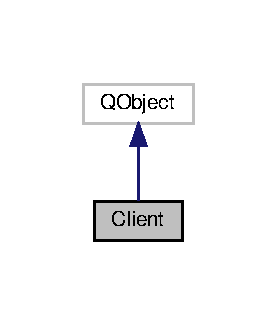
\includegraphics[width=133pt]{classClient__inherit__graph}
\end{center}
\end{figure}


Граф связей класса Client\+:\nopagebreak
\begin{figure}[H]
\begin{center}
\leavevmode
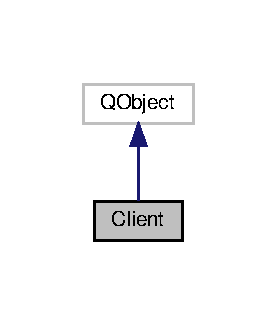
\includegraphics[width=133pt]{classClient__coll__graph}
\end{center}
\end{figure}
\subsection*{Открытые слоты}
\begin{DoxyCompactItemize}
\item 
void \hyperlink{classClient_a5f3de6434245dc99ceac8601806cb6b1}{connected} ()
\begin{DoxyCompactList}\small\item\em connected \end{DoxyCompactList}\item 
void \hyperlink{classClient_ac2cdeb8b0249c1bf0ddd2167da861ad4}{disconnected} ()
\begin{DoxyCompactList}\small\item\em disconnected \end{DoxyCompactList}\item 
void \hyperlink{classClient_acfd4db27c0fec82a26e4d112b585b534}{ready\+Read} ()
\begin{DoxyCompactList}\small\item\em ready\+Read Слот для записи в лог факта готовности к обмену информацией \end{DoxyCompactList}\item 
void \hyperlink{classClient_a21d8173cfcb182fe554a0828c5dea8be}{Task\+Result} (Q\+Byte\+Array ba)
\begin{DoxyCompactList}\small\item\em Task\+Result. \end{DoxyCompactList}\end{DoxyCompactItemize}
\subsection*{Сигналы}
\begin{DoxyCompactItemize}
\item 
void \hyperlink{classClient_ae73142778c856392f6b40803558461df}{transfer\+Data\+To\+Server} (Q\+Byte\+Array ba)
\begin{DoxyCompactList}\small\item\em transfer\+Data\+To\+Server \end{DoxyCompactList}\end{DoxyCompactItemize}
\subsection*{Открытые члены}
\begin{DoxyCompactItemize}
\item 
\hyperlink{classClient_a5b62b1caeb5c2c35a2ae367851d3ad92}{Client} (Q\+Object $\ast$parent=nullptr)
\begin{DoxyCompactList}\small\item\em \hyperlink{classClient}{Client}. \end{DoxyCompactList}\item 
void \hyperlink{classClient_a38b742b4f0fbb661f4884686899ea5c2}{set\+Socket} (qintptr Descriptor)
\begin{DoxyCompactList}\small\item\em set\+Socket \end{DoxyCompactList}\end{DoxyCompactItemize}
\subsection*{Закрытые данные}
\begin{DoxyCompactItemize}
\item 
Q\+Tcp\+Socket $\ast$ \hyperlink{classClient_acfb33719fbe6b0685ca7324c0ee893c5}{socket}
\begin{DoxyCompactList}\small\item\em socket \end{DoxyCompactList}\item 
const int \hyperlink{classClient_a61dd7284140818bcb19dbd5bcccec846}{m\+\_\+max\+\_\+thread\+\_\+count} = 5
\begin{DoxyCompactList}\small\item\em m\+\_\+max\+\_\+thread\+\_\+count \end{DoxyCompactList}\end{DoxyCompactItemize}


\subsection{Подробное описание}
Класс имитирующий клиента подключенного к серверу 

\begin{DoxyAuthor}{Автор}
Илья Трефилов 
\end{DoxyAuthor}
\begin{DoxyDate}{Дата}
01.\+12.\+2018
\end{DoxyDate}
Данный класс предназначен для сохранения и обработки информации от подключенного клиента с сохранением контекста 

\subsection{Конструктор(ы)}
\mbox{\Hypertarget{classClient_a5b62b1caeb5c2c35a2ae367851d3ad92}\label{classClient_a5b62b1caeb5c2c35a2ae367851d3ad92}} 
\index{Client@{Client}!Client@{Client}}
\index{Client@{Client}!Client@{Client}}
\subsubsection{\texorpdfstring{Client()}{Client()}}
{\footnotesize\ttfamily Client\+::\+Client (\begin{DoxyParamCaption}\item[{Q\+Object $\ast$}]{parent = {\ttfamily nullptr} }\end{DoxyParamCaption})\hspace{0.3cm}{\ttfamily [explicit]}}



\hyperlink{classClient}{Client}. 


\begin{DoxyParams}{Аргументы}
{\em parent} & Ссылка на родительский объект типа Q\+Object\\
\hline
\end{DoxyParams}
Конструктор класса \hyperlink{classClient}{Client} 

\subsection{Методы}
\mbox{\Hypertarget{classClient_a5f3de6434245dc99ceac8601806cb6b1}\label{classClient_a5f3de6434245dc99ceac8601806cb6b1}} 
\index{Client@{Client}!connected@{connected}}
\index{connected@{connected}!Client@{Client}}
\subsubsection{\texorpdfstring{connected}{connected}}
{\footnotesize\ttfamily void Client\+::connected (\begin{DoxyParamCaption}{ }\end{DoxyParamCaption})\hspace{0.3cm}{\ttfamily [slot]}}



connected 

Слот для записи в лог факт соединения с клиентом \mbox{\Hypertarget{classClient_ac2cdeb8b0249c1bf0ddd2167da861ad4}\label{classClient_ac2cdeb8b0249c1bf0ddd2167da861ad4}} 
\index{Client@{Client}!disconnected@{disconnected}}
\index{disconnected@{disconnected}!Client@{Client}}
\subsubsection{\texorpdfstring{disconnected}{disconnected}}
{\footnotesize\ttfamily void Client\+::disconnected (\begin{DoxyParamCaption}{ }\end{DoxyParamCaption})\hspace{0.3cm}{\ttfamily [slot]}}



disconnected 

Слот для записи в лог факт о завершении соединения с клиентом \mbox{\Hypertarget{classClient_acfd4db27c0fec82a26e4d112b585b534}\label{classClient_acfd4db27c0fec82a26e4d112b585b534}} 
\index{Client@{Client}!ready\+Read@{ready\+Read}}
\index{ready\+Read@{ready\+Read}!Client@{Client}}
\subsubsection{\texorpdfstring{ready\+Read}{readyRead}}
{\footnotesize\ttfamily void Client\+::ready\+Read (\begin{DoxyParamCaption}{ }\end{DoxyParamCaption})\hspace{0.3cm}{\ttfamily [slot]}}



ready\+Read Слот для записи в лог факта готовности к обмену информацией 

\mbox{\Hypertarget{classClient_a38b742b4f0fbb661f4884686899ea5c2}\label{classClient_a38b742b4f0fbb661f4884686899ea5c2}} 
\index{Client@{Client}!set\+Socket@{set\+Socket}}
\index{set\+Socket@{set\+Socket}!Client@{Client}}
\subsubsection{\texorpdfstring{set\+Socket()}{setSocket()}}
{\footnotesize\ttfamily void Client\+::set\+Socket (\begin{DoxyParamCaption}\item[{qintptr}]{Descriptor }\end{DoxyParamCaption})}



set\+Socket 


\begin{DoxyParams}{Аргументы}
{\em Descriptor} & Дескриптор открытого для соединения сокета\\
\hline
\end{DoxyParams}
Данная функция создает сокет при подключении клиента к серверу \mbox{\Hypertarget{classClient_a21d8173cfcb182fe554a0828c5dea8be}\label{classClient_a21d8173cfcb182fe554a0828c5dea8be}} 
\index{Client@{Client}!Task\+Result@{Task\+Result}}
\index{Task\+Result@{Task\+Result}!Client@{Client}}
\subsubsection{\texorpdfstring{Task\+Result}{TaskResult}}
{\footnotesize\ttfamily void Client\+::\+Task\+Result (\begin{DoxyParamCaption}\item[{Q\+Byte\+Array}]{ba }\end{DoxyParamCaption})\hspace{0.3cm}{\ttfamily [slot]}}



Task\+Result. 


\begin{DoxyParams}{Аргументы}
{\em ba} & Набор байт записанный клиентом в сокет\\
\hline
\end{DoxyParams}
Слот для записи в лог полученной информации и вызова сигнала для передачи информации классу сервера \mbox{\Hypertarget{classClient_ae73142778c856392f6b40803558461df}\label{classClient_ae73142778c856392f6b40803558461df}} 
\index{Client@{Client}!transfer\+Data\+To\+Server@{transfer\+Data\+To\+Server}}
\index{transfer\+Data\+To\+Server@{transfer\+Data\+To\+Server}!Client@{Client}}
\subsubsection{\texorpdfstring{transfer\+Data\+To\+Server}{transferDataToServer}}
{\footnotesize\ttfamily void Client\+::transfer\+Data\+To\+Server (\begin{DoxyParamCaption}\item[{Q\+Byte\+Array}]{ba }\end{DoxyParamCaption})\hspace{0.3cm}{\ttfamily [signal]}}



transfer\+Data\+To\+Server 


\begin{DoxyParams}{Аргументы}
{\em ba} & Набор байт записанный клиентом в сокет\\
\hline
\end{DoxyParams}
Сигнал отправки полученных данных классу сервера 

\subsection{Данные класса}
\mbox{\Hypertarget{classClient_a61dd7284140818bcb19dbd5bcccec846}\label{classClient_a61dd7284140818bcb19dbd5bcccec846}} 
\index{Client@{Client}!m\+\_\+max\+\_\+thread\+\_\+count@{m\+\_\+max\+\_\+thread\+\_\+count}}
\index{m\+\_\+max\+\_\+thread\+\_\+count@{m\+\_\+max\+\_\+thread\+\_\+count}!Client@{Client}}
\subsubsection{\texorpdfstring{m\+\_\+max\+\_\+thread\+\_\+count}{m\_max\_thread\_count}}
{\footnotesize\ttfamily const int Client\+::m\+\_\+max\+\_\+thread\+\_\+count = 5\hspace{0.3cm}{\ttfamily [private]}}



m\+\_\+max\+\_\+thread\+\_\+count 

Константа ограничивающая максимальное количество одновременных потоков для обработки информации. Константа создает ограничение на количество одновременно подключенных пользователей \mbox{\Hypertarget{classClient_acfb33719fbe6b0685ca7324c0ee893c5}\label{classClient_acfb33719fbe6b0685ca7324c0ee893c5}} 
\index{Client@{Client}!socket@{socket}}
\index{socket@{socket}!Client@{Client}}
\subsubsection{\texorpdfstring{socket}{socket}}
{\footnotesize\ttfamily Q\+Tcp\+Socket$\ast$ Client\+::socket\hspace{0.3cm}{\ttfamily [private]}}



socket 

Указатель на открытый для соединения сокет 

Объявления и описания членов классов находятся в файлах\+:\begin{DoxyCompactItemize}
\item 
\hyperlink{client_8h}{client.\+h}\item 
\hyperlink{client_8cpp}{client.\+cpp}\end{DoxyCompactItemize}

\hypertarget{classDbForm}{}\section{Класс Db\+Form}
\label{classDbForm}\index{Db\+Form@{Db\+Form}}


Класс формы для отображения содержимого базы данных  




{\ttfamily \#include $<$dbform.\+h$>$}



Граф наследования\+:Db\+Form\+:\nopagebreak
\begin{figure}[H]
\begin{center}
\leavevmode
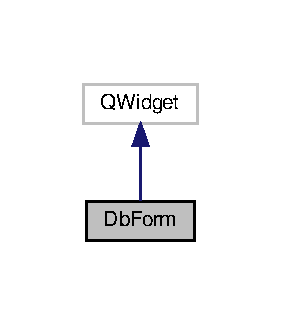
\includegraphics[width=135pt]{classDbForm__inherit__graph}
\end{center}
\end{figure}


Граф связей класса Db\+Form\+:\nopagebreak
\begin{figure}[H]
\begin{center}
\leavevmode
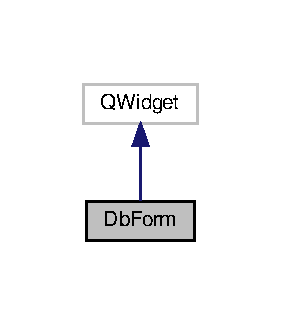
\includegraphics[width=135pt]{classDbForm__coll__graph}
\end{center}
\end{figure}
\subsection*{Открытые слоты}
\begin{DoxyCompactItemize}
\item 
void \hyperlink{classDbForm_af542d8df492aab988ff036022365f3fd}{accept\+Insert\+Signal} (Q\+String \&name, Q\+Image \&image, \hyperlink{tagshelpers_8h_ae25d30658f61420b88a380dc9e40bb74}{dicom\+Dict} \&dict, \hyperlink{dbform_8h_a1ec1a645f41e1c6544d384ca863a936c}{add\+Info\+Map} \&map)
\begin{DoxyCompactList}\small\item\em accept\+Insert\+Signal \end{DoxyCompactList}\end{DoxyCompactItemize}
\subsection*{Открытые члены}
\begin{DoxyCompactItemize}
\item 
\hyperlink{classDbForm_a66426b83490cb4c054905c12dc6a220e}{Db\+Form} (Q\+Widget $\ast$parent=nullptr)
\begin{DoxyCompactList}\small\item\em \hyperlink{classDbForm}{Db\+Form}. \end{DoxyCompactList}\item 
\hyperlink{classDbForm_abbdba78f6818adfd9fc156b3246bb788}{$\sim$\+Db\+Form} ()
\end{DoxyCompactItemize}
\subsection*{Открытые статические члены}
\begin{DoxyCompactItemize}
\item 
static void \hyperlink{classDbForm_a3877cc6e7b607e2999da50b5322615d4}{init\+Footer\+Table} (Q\+Table\+Widget $\ast$widget, const \hyperlink{tagshelpers_8h_ae25d30658f61420b88a380dc9e40bb74}{dicom\+Dict} \&dict)
\begin{DoxyCompactList}\small\item\em init\+Footer\+Table \end{DoxyCompactList}\end{DoxyCompactItemize}
\subsection*{Закрытые типы}
\begin{DoxyCompactItemize}
\item 
enum \hyperlink{classDbForm_a86764414aea9eeb51e9cdfa722447b93}{columns} \{ \hyperlink{classDbForm_a86764414aea9eeb51e9cdfa722447b93ab80bb7740288fda1f201890375a60c8f}{columns\+::id} = 0, 
\hyperlink{classDbForm_a86764414aea9eeb51e9cdfa722447b93ab068931cc450442b63f5b3d276ea4297}{columns\+::name} = 1, 
\hyperlink{classDbForm_a86764414aea9eeb51e9cdfa722447b93a78805a221a988e79ef3f42d7c5bfd418}{columns\+::image} = 2, 
\hyperlink{classDbForm_a86764414aea9eeb51e9cdfa722447b93a8d777f385d3dfec8815d20f7496026dc}{columns\+::data} = 3
 \}\begin{DoxyCompactList}\small\item\em The columns enum. \end{DoxyCompactList}
\item 
enum \hyperlink{classDbForm_a3c4b02b0603d0d9cd8c22ed0214d55fd}{dicom\+Columns} \{ \hyperlink{classDbForm_a3c4b02b0603d0d9cd8c22ed0214d55fdac49e86041d3f004eeaaff68fb53cd961}{tag}, 
\hyperlink{classDbForm_a3c4b02b0603d0d9cd8c22ed0214d55fdade3e2648868259c386f105866f10211b}{description}, 
\hyperlink{classDbForm_a3c4b02b0603d0d9cd8c22ed0214d55fda545ec36d06133ca13ccb0780da8184e9}{value}
 \}\begin{DoxyCompactList}\small\item\em The columns enum. \end{DoxyCompactList}
\end{DoxyCompactItemize}
\subsection*{Закрытые слоты}
\begin{DoxyCompactItemize}
\item 
void \hyperlink{classDbForm_ae26fa6d6d1be86e8fff9766d64392fdd}{on\+\_\+db\+Table\+Widget\+\_\+cell\+Clicked} (int row, int column)
\begin{DoxyCompactList}\small\item\em on\+\_\+db\+Table\+Widget\+\_\+cell\+Clicked \end{DoxyCompactList}\item 
void \hyperlink{classDbForm_aa1f2f6562e51324bb3dc453f9579380b}{on\+\_\+update\+Button\+\_\+clicked} ()
\begin{DoxyCompactList}\small\item\em on\+\_\+update\+Button\+\_\+clicked \end{DoxyCompactList}\end{DoxyCompactItemize}
\subsection*{Закрытые члены}
\begin{DoxyCompactItemize}
\item 
bool \hyperlink{classDbForm_a40fbf82d24dc0e20031aef14dc4a8366}{ask\+For\+Save} ()
\begin{DoxyCompactList}\small\item\em ask\+For\+Save \end{DoxyCompactList}\item 
void \hyperlink{classDbForm_a56e109480a6bd4556baaf369bc79f99f}{preview\+Image} (const int \&id)
\begin{DoxyCompactList}\small\item\em preview\+Image \end{DoxyCompactList}\item 
bool \hyperlink{classDbForm_af79b6454611a052e4da31db0bac13ed1}{init\+Table\+Widget} ()
\begin{DoxyCompactList}\small\item\em init\+Table\+Widget \end{DoxyCompactList}\item 
bool \hyperlink{classDbForm_a3453aae86a90552e3e7dd84b38315cc0}{dump\+To\+Db} (Q\+String \&name, Q\+Image \&image, \hyperlink{tagshelpers_8h_ae25d30658f61420b88a380dc9e40bb74}{dicom\+Dict} \&dict, \hyperlink{dbform_8h_a1ec1a645f41e1c6544d384ca863a936c}{add\+Info\+Map} \&map)
\begin{DoxyCompactList}\small\item\em dump\+To\+Db \end{DoxyCompactList}\item 
void \hyperlink{classDbForm_ab375348c98051eea969574da00484c29}{insert\+Additional\+Info} (Q\+Sql\+Query \&query, const \hyperlink{dbform_8h_a1ec1a645f41e1c6544d384ca863a936c}{add\+Info\+Map} \&map)
\begin{DoxyCompactList}\small\item\em insert\+Additional\+Info \end{DoxyCompactList}\end{DoxyCompactItemize}
\subsection*{Закрытые данные}
\begin{DoxyCompactItemize}
\item 
Ui\+::\+Db\+Form $\ast$ \hyperlink{classDbForm_a481b25bcbc8d2613cf09e786319e9559}{ui}
\begin{DoxyCompactList}\small\item\em ui \end{DoxyCompactList}\item 
const Q\+String \hyperlink{classDbForm_a8db1268928d78d414fd354cbc08c92c8}{m\+\_\+db\+Path}
\begin{DoxyCompactList}\small\item\em m\+\_\+db\+Path \end{DoxyCompactList}\item 
const Q\+String \hyperlink{classDbForm_a13a6b5d290951dfb001cfe34324c1634}{m\+\_\+db\+Table}
\begin{DoxyCompactList}\small\item\em m\+\_\+db\+Table \end{DoxyCompactList}\item 
const Q\+Icon \hyperlink{classDbForm_a8231b5e3687e61e8b3391040f99f33fe}{m\+\_\+ok\+Icon}
\begin{DoxyCompactList}\small\item\em m\+\_\+ok\+Icon \end{DoxyCompactList}\item 
const Q\+Icon \hyperlink{classDbForm_a664eef6253a7345bd09b820346c0e3c9}{m\+\_\+unavailable\+Icon}
\begin{DoxyCompactList}\small\item\em m\+\_\+unavailable\+Icon \end{DoxyCompactList}\item 
const Q\+Icon \hyperlink{classDbForm_ac2f11a495462056b06da8e3d62a04c22}{m\+\_\+update\+Icon}
\begin{DoxyCompactList}\small\item\em m\+\_\+update\+Icon \end{DoxyCompactList}\item 
Q\+Sql\+Database \hyperlink{classDbForm_a8baa011f5fa0625622b5930977ae8492}{m\+\_\+db}
\begin{DoxyCompactList}\small\item\em m\+\_\+db \end{DoxyCompactList}\item 
Q\+Graphics\+Scene \hyperlink{classDbForm_a2f5838603cedc772f92fc47cd484c93a}{m\+\_\+preview\+Scene}
\begin{DoxyCompactList}\small\item\em m\+\_\+preview\+Scene \end{DoxyCompactList}\end{DoxyCompactItemize}
\subsection*{Друзья}
\begin{DoxyCompactItemize}
\item 
class \hyperlink{classDbForm_a6f843022f5255cb942da23ecb29ae451}{Send\+Dialog}
\end{DoxyCompactItemize}


\subsection{Подробное описание}
Класс формы для отображения содержимого базы данных 

\begin{DoxyAuthor}{Автор}
Илья Трефилов 
\end{DoxyAuthor}
\begin{DoxyDate}{Дата}
01.\+12.\+2018
\end{DoxyDate}
Данный класс предназначен для отбражения информации, хранящейся в локальной базе о изученных объектах 

\subsection{Перечисления}
\mbox{\Hypertarget{classDbForm_a86764414aea9eeb51e9cdfa722447b93}\label{classDbForm_a86764414aea9eeb51e9cdfa722447b93}} 
\index{Db\+Form@{Db\+Form}!columns@{columns}}
\index{columns@{columns}!Db\+Form@{Db\+Form}}
\subsubsection{\texorpdfstring{columns}{columns}}
{\footnotesize\ttfamily enum \hyperlink{classDbForm_a86764414aea9eeb51e9cdfa722447b93}{Db\+Form\+::columns}\hspace{0.3cm}{\ttfamily [strong]}, {\ttfamily [private]}}



The columns enum. 

Перечисление столбцов таблицы для отображения числовых значений на смысловое содержание информации, хранящейся в таблице \begin{DoxyEnumFields}{Элементы перечислений}
\raisebox{\heightof{T}}[0pt][0pt]{\index{id@{id}!Db\+Form@{Db\+Form}}\index{Db\+Form@{Db\+Form}!id@{id}}}\mbox{\Hypertarget{classDbForm_a86764414aea9eeb51e9cdfa722447b93ab80bb7740288fda1f201890375a60c8f}\label{classDbForm_a86764414aea9eeb51e9cdfa722447b93ab80bb7740288fda1f201890375a60c8f}} 
id&\\
\hline

\raisebox{\heightof{T}}[0pt][0pt]{\index{name@{name}!Db\+Form@{Db\+Form}}\index{Db\+Form@{Db\+Form}!name@{name}}}\mbox{\Hypertarget{classDbForm_a86764414aea9eeb51e9cdfa722447b93ab068931cc450442b63f5b3d276ea4297}\label{classDbForm_a86764414aea9eeb51e9cdfa722447b93ab068931cc450442b63f5b3d276ea4297}} 
name&\\
\hline

\raisebox{\heightof{T}}[0pt][0pt]{\index{image@{image}!Db\+Form@{Db\+Form}}\index{Db\+Form@{Db\+Form}!image@{image}}}\mbox{\Hypertarget{classDbForm_a86764414aea9eeb51e9cdfa722447b93a78805a221a988e79ef3f42d7c5bfd418}\label{classDbForm_a86764414aea9eeb51e9cdfa722447b93a78805a221a988e79ef3f42d7c5bfd418}} 
image&\\
\hline

\raisebox{\heightof{T}}[0pt][0pt]{\index{data@{data}!Db\+Form@{Db\+Form}}\index{Db\+Form@{Db\+Form}!data@{data}}}\mbox{\Hypertarget{classDbForm_a86764414aea9eeb51e9cdfa722447b93a8d777f385d3dfec8815d20f7496026dc}\label{classDbForm_a86764414aea9eeb51e9cdfa722447b93a8d777f385d3dfec8815d20f7496026dc}} 
data&\\
\hline

\end{DoxyEnumFields}
\mbox{\Hypertarget{classDbForm_a3c4b02b0603d0d9cd8c22ed0214d55fd}\label{classDbForm_a3c4b02b0603d0d9cd8c22ed0214d55fd}} 
\index{Db\+Form@{Db\+Form}!dicom\+Columns@{dicom\+Columns}}
\index{dicom\+Columns@{dicom\+Columns}!Db\+Form@{Db\+Form}}
\subsubsection{\texorpdfstring{dicom\+Columns}{dicomColumns}}
{\footnotesize\ttfamily enum \hyperlink{classDbForm_a3c4b02b0603d0d9cd8c22ed0214d55fd}{Db\+Form\+::dicom\+Columns}\hspace{0.3cm}{\ttfamily [private]}}



The columns enum. 

Перечисление столбцов таблицы для отображения числовых значений на смысловое содержание информации, хранящейся в таблице \begin{DoxyEnumFields}{Элементы перечислений}
\raisebox{\heightof{T}}[0pt][0pt]{\index{tag@{tag}!Db\+Form@{Db\+Form}}\index{Db\+Form@{Db\+Form}!tag@{tag}}}\mbox{\Hypertarget{classDbForm_a3c4b02b0603d0d9cd8c22ed0214d55fdac49e86041d3f004eeaaff68fb53cd961}\label{classDbForm_a3c4b02b0603d0d9cd8c22ed0214d55fdac49e86041d3f004eeaaff68fb53cd961}} 
tag&\\
\hline

\raisebox{\heightof{T}}[0pt][0pt]{\index{description@{description}!Db\+Form@{Db\+Form}}\index{Db\+Form@{Db\+Form}!description@{description}}}\mbox{\Hypertarget{classDbForm_a3c4b02b0603d0d9cd8c22ed0214d55fdade3e2648868259c386f105866f10211b}\label{classDbForm_a3c4b02b0603d0d9cd8c22ed0214d55fdade3e2648868259c386f105866f10211b}} 
description&\\
\hline

\raisebox{\heightof{T}}[0pt][0pt]{\index{value@{value}!Db\+Form@{Db\+Form}}\index{Db\+Form@{Db\+Form}!value@{value}}}\mbox{\Hypertarget{classDbForm_a3c4b02b0603d0d9cd8c22ed0214d55fda545ec36d06133ca13ccb0780da8184e9}\label{classDbForm_a3c4b02b0603d0d9cd8c22ed0214d55fda545ec36d06133ca13ccb0780da8184e9}} 
value&\\
\hline

\end{DoxyEnumFields}


\subsection{Конструктор(ы)}
\mbox{\Hypertarget{classDbForm_a66426b83490cb4c054905c12dc6a220e}\label{classDbForm_a66426b83490cb4c054905c12dc6a220e}} 
\index{Db\+Form@{Db\+Form}!Db\+Form@{Db\+Form}}
\index{Db\+Form@{Db\+Form}!Db\+Form@{Db\+Form}}
\subsubsection{\texorpdfstring{Db\+Form()}{DbForm()}}
{\footnotesize\ttfamily Db\+Form\+::\+Db\+Form (\begin{DoxyParamCaption}\item[{Q\+Widget $\ast$}]{parent = {\ttfamily nullptr} }\end{DoxyParamCaption})\hspace{0.3cm}{\ttfamily [explicit]}}



\hyperlink{classDbForm}{Db\+Form}. 


\begin{DoxyParams}{Аргументы}
{\em parent} & Указатель на родительский класс -\/ виджет\\
\hline
\end{DoxyParams}
Конструктор виджета \mbox{\Hypertarget{classDbForm_abbdba78f6818adfd9fc156b3246bb788}\label{classDbForm_abbdba78f6818adfd9fc156b3246bb788}} 
\index{Db\+Form@{Db\+Form}!````~Db\+Form@{$\sim$\+Db\+Form}}
\index{````~Db\+Form@{$\sim$\+Db\+Form}!Db\+Form@{Db\+Form}}
\subsubsection{\texorpdfstring{$\sim$\+Db\+Form()}{~DbForm()}}
{\footnotesize\ttfamily Db\+Form\+::$\sim$\+Db\+Form (\begin{DoxyParamCaption}{ }\end{DoxyParamCaption})}



\subsection{Методы}
\mbox{\Hypertarget{classDbForm_af542d8df492aab988ff036022365f3fd}\label{classDbForm_af542d8df492aab988ff036022365f3fd}} 
\index{Db\+Form@{Db\+Form}!accept\+Insert\+Signal@{accept\+Insert\+Signal}}
\index{accept\+Insert\+Signal@{accept\+Insert\+Signal}!Db\+Form@{Db\+Form}}
\subsubsection{\texorpdfstring{accept\+Insert\+Signal}{acceptInsertSignal}}
{\footnotesize\ttfamily void Db\+Form\+::accept\+Insert\+Signal (\begin{DoxyParamCaption}\item[{Q\+String \&}]{name,  }\item[{Q\+Image \&}]{image,  }\item[{\hyperlink{tagshelpers_8h_ae25d30658f61420b88a380dc9e40bb74}{dicom\+Dict} \&}]{dict,  }\item[{\hyperlink{dbform_8h_a1ec1a645f41e1c6544d384ca863a936c}{add\+Info\+Map} \&}]{map }\end{DoxyParamCaption})\hspace{0.3cm}{\ttfamily [slot]}}



accept\+Insert\+Signal 


\begin{DoxyParams}{Аргументы}
{\em name} & Имя пациента \\
\hline
{\em image} & Медицинское изображение \\
\hline
{\em dict} & Словарь содержащий информацию о dicom объекте \\
\hline
{\em map} & Словарь содержащий дополнительную информацию о запросе\textbackslash{}ответе\\
\hline
\end{DoxyParams}
Слот для приема сигнала о необходимости записи объекта в базу данных \mbox{\Hypertarget{classDbForm_a40fbf82d24dc0e20031aef14dc4a8366}\label{classDbForm_a40fbf82d24dc0e20031aef14dc4a8366}} 
\index{Db\+Form@{Db\+Form}!ask\+For\+Save@{ask\+For\+Save}}
\index{ask\+For\+Save@{ask\+For\+Save}!Db\+Form@{Db\+Form}}
\subsubsection{\texorpdfstring{ask\+For\+Save()}{askForSave()}}
{\footnotesize\ttfamily bool Db\+Form\+::ask\+For\+Save (\begin{DoxyParamCaption}{ }\end{DoxyParamCaption})\hspace{0.3cm}{\ttfamily [private]}}



ask\+For\+Save 

\begin{DoxyReturn}{Возвращает}
Возвращает значение типа boolean, указывающее на необходимость сохранения в базу данных
\end{DoxyReturn}
Если функция вернула true -\/ посылаем сигнал сохранения в базу данных \mbox{\Hypertarget{classDbForm_a3453aae86a90552e3e7dd84b38315cc0}\label{classDbForm_a3453aae86a90552e3e7dd84b38315cc0}} 
\index{Db\+Form@{Db\+Form}!dump\+To\+Db@{dump\+To\+Db}}
\index{dump\+To\+Db@{dump\+To\+Db}!Db\+Form@{Db\+Form}}
\subsubsection{\texorpdfstring{dump\+To\+Db()}{dumpToDb()}}
{\footnotesize\ttfamily bool Db\+Form\+::dump\+To\+Db (\begin{DoxyParamCaption}\item[{Q\+String \&}]{name,  }\item[{Q\+Image \&}]{image,  }\item[{\hyperlink{tagshelpers_8h_ae25d30658f61420b88a380dc9e40bb74}{dicom\+Dict} \&}]{dict,  }\item[{\hyperlink{dbform_8h_a1ec1a645f41e1c6544d384ca863a936c}{add\+Info\+Map} \&}]{map }\end{DoxyParamCaption})\hspace{0.3cm}{\ttfamily [private]}}



dump\+To\+Db 


\begin{DoxyParams}{Аргументы}
{\em name} & Имя пациента \\
\hline
{\em image} & Медицинское изображение \\
\hline
{\em dict} & Словарь для хранения информации dicom \\
\hline
{\em map} & Словарь с дополнительными данных о запросе\textbackslash{}ответе \\
\hline
\end{DoxyParams}
\begin{DoxyReturn}{Возвращает}
true -\/ если запись в базу прошла успешно
\end{DoxyReturn}
Функция для записи в базу информации о запросе\textbackslash{}ответе \mbox{\Hypertarget{classDbForm_a3877cc6e7b607e2999da50b5322615d4}\label{classDbForm_a3877cc6e7b607e2999da50b5322615d4}} 
\index{Db\+Form@{Db\+Form}!init\+Footer\+Table@{init\+Footer\+Table}}
\index{init\+Footer\+Table@{init\+Footer\+Table}!Db\+Form@{Db\+Form}}
\subsubsection{\texorpdfstring{init\+Footer\+Table()}{initFooterTable()}}
{\footnotesize\ttfamily void Db\+Form\+::init\+Footer\+Table (\begin{DoxyParamCaption}\item[{Q\+Table\+Widget $\ast$}]{widget,  }\item[{const \hyperlink{tagshelpers_8h_ae25d30658f61420b88a380dc9e40bb74}{dicom\+Dict} \&}]{dict }\end{DoxyParamCaption})\hspace{0.3cm}{\ttfamily [static]}}



init\+Footer\+Table 


\begin{DoxyParams}{Аргументы}
{\em widget} & Ссылка на виджет типа таблицы \\
\hline
{\em dict} & Словарь содержащий информацию о dicom объекте \\
\hline
\end{DoxyParams}
\mbox{\Hypertarget{classDbForm_af79b6454611a052e4da31db0bac13ed1}\label{classDbForm_af79b6454611a052e4da31db0bac13ed1}} 
\index{Db\+Form@{Db\+Form}!init\+Table\+Widget@{init\+Table\+Widget}}
\index{init\+Table\+Widget@{init\+Table\+Widget}!Db\+Form@{Db\+Form}}
\subsubsection{\texorpdfstring{init\+Table\+Widget()}{initTableWidget()}}
{\footnotesize\ttfamily bool Db\+Form\+::init\+Table\+Widget (\begin{DoxyParamCaption}{ }\end{DoxyParamCaption})\hspace{0.3cm}{\ttfamily [private]}}



init\+Table\+Widget 

\begin{DoxyReturn}{Возвращает}
true, если таблица информации в базе данных успешно инициализировалась из базы данных
\end{DoxyReturn}
Функция для инициализации таблицы информацией из базы данных \mbox{\Hypertarget{classDbForm_ab375348c98051eea969574da00484c29}\label{classDbForm_ab375348c98051eea969574da00484c29}} 
\index{Db\+Form@{Db\+Form}!insert\+Additional\+Info@{insert\+Additional\+Info}}
\index{insert\+Additional\+Info@{insert\+Additional\+Info}!Db\+Form@{Db\+Form}}
\subsubsection{\texorpdfstring{insert\+Additional\+Info()}{insertAdditionalInfo()}}
{\footnotesize\ttfamily void Db\+Form\+::insert\+Additional\+Info (\begin{DoxyParamCaption}\item[{Q\+Sql\+Query \&}]{query,  }\item[{const \hyperlink{dbform_8h_a1ec1a645f41e1c6544d384ca863a936c}{add\+Info\+Map} \&}]{map }\end{DoxyParamCaption})\hspace{0.3cm}{\ttfamily [private]}}



insert\+Additional\+Info 


\begin{DoxyParams}{Аргументы}
{\em query} & Объект запроса в базу данных \\
\hline
{\em map} & Словарь с дополнительными данных о запросе\textbackslash{}ответе\\
\hline
\end{DoxyParams}
Функция записывает информацию о запросе\textbackslash{}ответе в базу данных \mbox{\Hypertarget{classDbForm_ae26fa6d6d1be86e8fff9766d64392fdd}\label{classDbForm_ae26fa6d6d1be86e8fff9766d64392fdd}} 
\index{Db\+Form@{Db\+Form}!on\+\_\+db\+Table\+Widget\+\_\+cell\+Clicked@{on\+\_\+db\+Table\+Widget\+\_\+cell\+Clicked}}
\index{on\+\_\+db\+Table\+Widget\+\_\+cell\+Clicked@{on\+\_\+db\+Table\+Widget\+\_\+cell\+Clicked}!Db\+Form@{Db\+Form}}
\subsubsection{\texorpdfstring{on\+\_\+db\+Table\+Widget\+\_\+cell\+Clicked}{on\_dbTableWidget\_cellClicked}}
{\footnotesize\ttfamily void Db\+Form\+::on\+\_\+db\+Table\+Widget\+\_\+cell\+Clicked (\begin{DoxyParamCaption}\item[{int}]{row,  }\item[{int}]{column }\end{DoxyParamCaption})\hspace{0.3cm}{\ttfamily [private]}, {\ttfamily [slot]}}



on\+\_\+db\+Table\+Widget\+\_\+cell\+Clicked 


\begin{DoxyParams}{Аргументы}
{\em row} & Номер строки таблицы \\
\hline
{\em column} & Номер столбца таблицы\\
\hline
\end{DoxyParams}
Слот для отображения информации в виджете при клике на соответсвующий объект из таблицы \mbox{\Hypertarget{classDbForm_aa1f2f6562e51324bb3dc453f9579380b}\label{classDbForm_aa1f2f6562e51324bb3dc453f9579380b}} 
\index{Db\+Form@{Db\+Form}!on\+\_\+update\+Button\+\_\+clicked@{on\+\_\+update\+Button\+\_\+clicked}}
\index{on\+\_\+update\+Button\+\_\+clicked@{on\+\_\+update\+Button\+\_\+clicked}!Db\+Form@{Db\+Form}}
\subsubsection{\texorpdfstring{on\+\_\+update\+Button\+\_\+clicked}{on\_updateButton\_clicked}}
{\footnotesize\ttfamily void Db\+Form\+::on\+\_\+update\+Button\+\_\+clicked (\begin{DoxyParamCaption}{ }\end{DoxyParamCaption})\hspace{0.3cm}{\ttfamily [private]}, {\ttfamily [slot]}}



on\+\_\+update\+Button\+\_\+clicked 

Слот для синхронизации таблицы в виджете и информации в базе данных \mbox{\Hypertarget{classDbForm_a56e109480a6bd4556baaf369bc79f99f}\label{classDbForm_a56e109480a6bd4556baaf369bc79f99f}} 
\index{Db\+Form@{Db\+Form}!preview\+Image@{preview\+Image}}
\index{preview\+Image@{preview\+Image}!Db\+Form@{Db\+Form}}
\subsubsection{\texorpdfstring{preview\+Image()}{previewImage()}}
{\footnotesize\ttfamily void Db\+Form\+::preview\+Image (\begin{DoxyParamCaption}\item[{const int \&}]{id }\end{DoxyParamCaption})\hspace{0.3cm}{\ttfamily [private]}}



preview\+Image 


\begin{DoxyParams}{Аргументы}
{\em id} & Номер объекта в базе данных\\
\hline
\end{DoxyParams}
Функция для отображения изображения в виджете, по выбранному номеру объекта 

\subsection{Документация по друзьям класса и функциям, относящимся к классу}
\mbox{\Hypertarget{classDbForm_a6f843022f5255cb942da23ecb29ae451}\label{classDbForm_a6f843022f5255cb942da23ecb29ae451}} 
\index{Db\+Form@{Db\+Form}!Send\+Dialog@{Send\+Dialog}}
\index{Send\+Dialog@{Send\+Dialog}!Db\+Form@{Db\+Form}}
\subsubsection{\texorpdfstring{Send\+Dialog}{SendDialog}}
{\footnotesize\ttfamily friend class \hyperlink{classSendDialog}{Send\+Dialog}\hspace{0.3cm}{\ttfamily [friend]}}

Объявления класса \hyperlink{classSendDialog}{Send\+Dialog} дружественным классом для предоставления форме \hyperlink{classSendDialog}{Send\+Dialog} доступа к БД средствами данного класса 

\subsection{Данные класса}
\mbox{\Hypertarget{classDbForm_a8baa011f5fa0625622b5930977ae8492}\label{classDbForm_a8baa011f5fa0625622b5930977ae8492}} 
\index{Db\+Form@{Db\+Form}!m\+\_\+db@{m\+\_\+db}}
\index{m\+\_\+db@{m\+\_\+db}!Db\+Form@{Db\+Form}}
\subsubsection{\texorpdfstring{m\+\_\+db}{m\_db}}
{\footnotesize\ttfamily Q\+Sql\+Database Db\+Form\+::m\+\_\+db\hspace{0.3cm}{\ttfamily [private]}}



m\+\_\+db 

Объект открытой программой базы данных \mbox{\Hypertarget{classDbForm_a8db1268928d78d414fd354cbc08c92c8}\label{classDbForm_a8db1268928d78d414fd354cbc08c92c8}} 
\index{Db\+Form@{Db\+Form}!m\+\_\+db\+Path@{m\+\_\+db\+Path}}
\index{m\+\_\+db\+Path@{m\+\_\+db\+Path}!Db\+Form@{Db\+Form}}
\subsubsection{\texorpdfstring{m\+\_\+db\+Path}{m\_dbPath}}
{\footnotesize\ttfamily const Q\+String Db\+Form\+::m\+\_\+db\+Path\hspace{0.3cm}{\ttfamily [private]}}



m\+\_\+db\+Path 

Константа, хранящая путь до базы данных \mbox{\Hypertarget{classDbForm_a13a6b5d290951dfb001cfe34324c1634}\label{classDbForm_a13a6b5d290951dfb001cfe34324c1634}} 
\index{Db\+Form@{Db\+Form}!m\+\_\+db\+Table@{m\+\_\+db\+Table}}
\index{m\+\_\+db\+Table@{m\+\_\+db\+Table}!Db\+Form@{Db\+Form}}
\subsubsection{\texorpdfstring{m\+\_\+db\+Table}{m\_dbTable}}
{\footnotesize\ttfamily const Q\+String Db\+Form\+::m\+\_\+db\+Table\hspace{0.3cm}{\ttfamily [private]}}



m\+\_\+db\+Table 

Константа, хранящая название таблицы \mbox{\Hypertarget{classDbForm_a8231b5e3687e61e8b3391040f99f33fe}\label{classDbForm_a8231b5e3687e61e8b3391040f99f33fe}} 
\index{Db\+Form@{Db\+Form}!m\+\_\+ok\+Icon@{m\+\_\+ok\+Icon}}
\index{m\+\_\+ok\+Icon@{m\+\_\+ok\+Icon}!Db\+Form@{Db\+Form}}
\subsubsection{\texorpdfstring{m\+\_\+ok\+Icon}{m\_okIcon}}
{\footnotesize\ttfamily const Q\+Icon Db\+Form\+::m\+\_\+ok\+Icon\hspace{0.3cm}{\ttfamily [private]}}



m\+\_\+ok\+Icon 

Константа, хранящая иконку, отображающую наличие информации в базе данных \mbox{\Hypertarget{classDbForm_a2f5838603cedc772f92fc47cd484c93a}\label{classDbForm_a2f5838603cedc772f92fc47cd484c93a}} 
\index{Db\+Form@{Db\+Form}!m\+\_\+preview\+Scene@{m\+\_\+preview\+Scene}}
\index{m\+\_\+preview\+Scene@{m\+\_\+preview\+Scene}!Db\+Form@{Db\+Form}}
\subsubsection{\texorpdfstring{m\+\_\+preview\+Scene}{m\_previewScene}}
{\footnotesize\ttfamily Q\+Graphics\+Scene Db\+Form\+::m\+\_\+preview\+Scene\hspace{0.3cm}{\ttfamily [private]}}



m\+\_\+preview\+Scene 

Сцена для демонстрации изображения в виджете из базы данных \mbox{\Hypertarget{classDbForm_a664eef6253a7345bd09b820346c0e3c9}\label{classDbForm_a664eef6253a7345bd09b820346c0e3c9}} 
\index{Db\+Form@{Db\+Form}!m\+\_\+unavailable\+Icon@{m\+\_\+unavailable\+Icon}}
\index{m\+\_\+unavailable\+Icon@{m\+\_\+unavailable\+Icon}!Db\+Form@{Db\+Form}}
\subsubsection{\texorpdfstring{m\+\_\+unavailable\+Icon}{m\_unavailableIcon}}
{\footnotesize\ttfamily const Q\+Icon Db\+Form\+::m\+\_\+unavailable\+Icon\hspace{0.3cm}{\ttfamily [private]}}



m\+\_\+unavailable\+Icon 

Константа, хранящая иконку, отображающую отсутствие информации в базе данных \mbox{\Hypertarget{classDbForm_ac2f11a495462056b06da8e3d62a04c22}\label{classDbForm_ac2f11a495462056b06da8e3d62a04c22}} 
\index{Db\+Form@{Db\+Form}!m\+\_\+update\+Icon@{m\+\_\+update\+Icon}}
\index{m\+\_\+update\+Icon@{m\+\_\+update\+Icon}!Db\+Form@{Db\+Form}}
\subsubsection{\texorpdfstring{m\+\_\+update\+Icon}{m\_updateIcon}}
{\footnotesize\ttfamily const Q\+Icon Db\+Form\+::m\+\_\+update\+Icon\hspace{0.3cm}{\ttfamily [private]}}



m\+\_\+update\+Icon 

Константа, хранящая иконку для обновления данных в виджете. Используется на кнопке обновления данных \mbox{\Hypertarget{classDbForm_a481b25bcbc8d2613cf09e786319e9559}\label{classDbForm_a481b25bcbc8d2613cf09e786319e9559}} 
\index{Db\+Form@{Db\+Form}!ui@{ui}}
\index{ui@{ui}!Db\+Form@{Db\+Form}}
\subsubsection{\texorpdfstring{ui}{ui}}
{\footnotesize\ttfamily Ui\+::\+Db\+Form$\ast$ Db\+Form\+::ui\hspace{0.3cm}{\ttfamily [private]}}



ui 

Ссылка на объект интерфейса для данной формы 

Объявления и описания членов классов находятся в файлах\+:\begin{DoxyCompactItemize}
\item 
\hyperlink{dbform_8h}{dbform.\+h}\item 
\hyperlink{dbform_8cpp}{dbform.\+cpp}\end{DoxyCompactItemize}

\hypertarget{classMainWindow}{}\section{Класс Main\+Window}
\label{classMainWindow}\index{Main\+Window@{Main\+Window}}


Класс главного окна программы.  




{\ttfamily \#include $<$mainwindow.\+h$>$}



Граф наследования\+:Main\+Window\+:\nopagebreak
\begin{figure}[H]
\begin{center}
\leavevmode
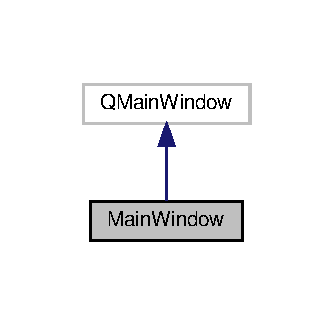
\includegraphics[width=160pt]{classMainWindow__inherit__graph}
\end{center}
\end{figure}


Граф связей класса Main\+Window\+:\nopagebreak
\begin{figure}[H]
\begin{center}
\leavevmode
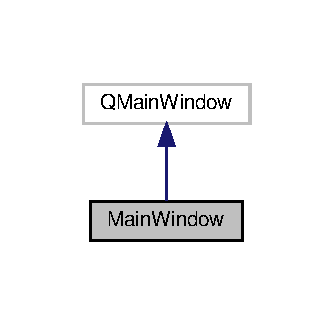
\includegraphics[width=160pt]{classMainWindow__coll__graph}
\end{center}
\end{figure}
\subsection*{Открытые члены}
\begin{DoxyCompactItemize}
\item 
void \hyperlink{classMainWindow_a3dea38a93f87d0ee9452035a4c9b8b7b}{init\+Sidebar} ()
\begin{DoxyCompactList}\small\item\em init\+Sidebar \end{DoxyCompactList}\item 
\hyperlink{classMainWindow_a996c5a2b6f77944776856f08ec30858d}{Main\+Window} (Q\+Widget $\ast$parent=nullptr)
\begin{DoxyCompactList}\small\item\em \hyperlink{classMainWindow}{Main\+Window}. \end{DoxyCompactList}\item 
\hyperlink{classMainWindow_ae98d00a93bc118200eeef9f9bba1dba7}{$\sim$\+Main\+Window} ()
\end{DoxyCompactItemize}
\subsection*{Открытые атрибуты}
\begin{DoxyCompactItemize}
\item 
Q\+String \hyperlink{classMainWindow_a06968aebc42a16ab51c5888b4784075d}{file\+Name}
\begin{DoxyCompactList}\small\item\em file\+Name \end{DoxyCompactList}\end{DoxyCompactItemize}
\subsection*{Закрытые слоты}
\begin{DoxyCompactItemize}
\item 
void \hyperlink{classMainWindow_aa9f8c5c52b9f244da93730fa8af5ed34}{display\+Viewer\+Layout} ()
\begin{DoxyCompactList}\small\item\em display\+Viewer\+Layout \end{DoxyCompactList}\item 
void \hyperlink{classMainWindow_ab8b823d0d84f50c5f243720f44471a7f}{display\+Db\+Layout} ()
\begin{DoxyCompactList}\small\item\em display\+Db\+Layout \end{DoxyCompactList}\item 
void \hyperlink{classMainWindow_a0f4b0fd14e2af4b462223612ed22c695}{display\+Accessibility\+Layout} ()
\begin{DoxyCompactList}\small\item\em display\+Accessibility\+Layout \end{DoxyCompactList}\item 
void \hyperlink{classMainWindow_a3da5047b0ff5cf5c10a20174a99c420c}{get\+Data} (Q\+Byte\+Array block)
\begin{DoxyCompactList}\small\item\em get\+Data \end{DoxyCompactList}\end{DoxyCompactItemize}
\subsection*{Закрытые данные}
\begin{DoxyCompactItemize}
\item 
const int \hyperlink{classMainWindow_a46d1e00d9af1678f68303e2f04a6a541}{m\+\_\+standart\+X\+Geom} = 300
\begin{DoxyCompactList}\small\item\em m\+\_\+standart\+X\+Geom \end{DoxyCompactList}\item 
const int \hyperlink{classMainWindow_a8ff8787bb09d87248d74e152d2133926}{m\+\_\+standart\+Y\+Geom} = 24
\begin{DoxyCompactList}\small\item\em m\+\_\+standart\+Y\+Geom \end{DoxyCompactList}\item 
const int \hyperlink{classMainWindow_a2aa939210e4ccc0fdbec8fd7e4497617}{m\+\_\+standart\+Width} = 1051
\begin{DoxyCompactList}\small\item\em m\+\_\+standart\+Width \end{DoxyCompactList}\item 
const int \hyperlink{classMainWindow_a5ebb2638e7863a72adc4e6f75336bd77}{m\+\_\+standart\+Height} = 975
\begin{DoxyCompactList}\small\item\em m\+\_\+standart\+Height \end{DoxyCompactList}\item 
Ui\+::\+Main\+Window $\ast$ \hyperlink{classMainWindow_a35466a70ed47252a0191168126a352a5}{ui}
\begin{DoxyCompactList}\small\item\em ui \end{DoxyCompactList}\end{DoxyCompactItemize}


\subsection{Подробное описание}
Класс главного окна программы. 

\begin{DoxyAuthor}{Автор}
Илья Трефилов 
\end{DoxyAuthor}
\begin{DoxyDate}{Дата}
01.\+12.\+2018
\end{DoxyDate}
Данный класс предназначен для управления функциями главного окна приложения 

\subsection{Конструктор(ы)}
\mbox{\Hypertarget{classMainWindow_a996c5a2b6f77944776856f08ec30858d}\label{classMainWindow_a996c5a2b6f77944776856f08ec30858d}} 
\index{Main\+Window@{Main\+Window}!Main\+Window@{Main\+Window}}
\index{Main\+Window@{Main\+Window}!Main\+Window@{Main\+Window}}
\subsubsection{\texorpdfstring{Main\+Window()}{MainWindow()}}
{\footnotesize\ttfamily Main\+Window\+::\+Main\+Window (\begin{DoxyParamCaption}\item[{Q\+Widget $\ast$}]{parent = {\ttfamily nullptr} }\end{DoxyParamCaption})\hspace{0.3cm}{\ttfamily [explicit]}}



\hyperlink{classMainWindow}{Main\+Window}. 


\begin{DoxyParams}{Аргументы}
{\em parent} & Указатель на родительский класс виджет\\
\hline
\end{DoxyParams}
Конструктор класса главного окна приложения \mbox{\Hypertarget{classMainWindow_ae98d00a93bc118200eeef9f9bba1dba7}\label{classMainWindow_ae98d00a93bc118200eeef9f9bba1dba7}} 
\index{Main\+Window@{Main\+Window}!````~Main\+Window@{$\sim$\+Main\+Window}}
\index{````~Main\+Window@{$\sim$\+Main\+Window}!Main\+Window@{Main\+Window}}
\subsubsection{\texorpdfstring{$\sim$\+Main\+Window()}{~MainWindow()}}
{\footnotesize\ttfamily Main\+Window\+::$\sim$\+Main\+Window (\begin{DoxyParamCaption}{ }\end{DoxyParamCaption})}



\subsection{Методы}
\mbox{\Hypertarget{classMainWindow_a0f4b0fd14e2af4b462223612ed22c695}\label{classMainWindow_a0f4b0fd14e2af4b462223612ed22c695}} 
\index{Main\+Window@{Main\+Window}!display\+Accessibility\+Layout@{display\+Accessibility\+Layout}}
\index{display\+Accessibility\+Layout@{display\+Accessibility\+Layout}!Main\+Window@{Main\+Window}}
\subsubsection{\texorpdfstring{display\+Accessibility\+Layout}{displayAccessibilityLayout}}
{\footnotesize\ttfamily void Main\+Window\+::display\+Accessibility\+Layout (\begin{DoxyParamCaption}{ }\end{DoxyParamCaption})\hspace{0.3cm}{\ttfamily [private]}, {\ttfamily [slot]}}



display\+Accessibility\+Layout 

Слот для отображения виджета сетевого взаимодействия \mbox{\Hypertarget{classMainWindow_ab8b823d0d84f50c5f243720f44471a7f}\label{classMainWindow_ab8b823d0d84f50c5f243720f44471a7f}} 
\index{Main\+Window@{Main\+Window}!display\+Db\+Layout@{display\+Db\+Layout}}
\index{display\+Db\+Layout@{display\+Db\+Layout}!Main\+Window@{Main\+Window}}
\subsubsection{\texorpdfstring{display\+Db\+Layout}{displayDbLayout}}
{\footnotesize\ttfamily void Main\+Window\+::display\+Db\+Layout (\begin{DoxyParamCaption}{ }\end{DoxyParamCaption})\hspace{0.3cm}{\ttfamily [private]}, {\ttfamily [slot]}}



display\+Db\+Layout 

Слот для отображения виджета просмотра содержимго базы данных \mbox{\Hypertarget{classMainWindow_aa9f8c5c52b9f244da93730fa8af5ed34}\label{classMainWindow_aa9f8c5c52b9f244da93730fa8af5ed34}} 
\index{Main\+Window@{Main\+Window}!display\+Viewer\+Layout@{display\+Viewer\+Layout}}
\index{display\+Viewer\+Layout@{display\+Viewer\+Layout}!Main\+Window@{Main\+Window}}
\subsubsection{\texorpdfstring{display\+Viewer\+Layout}{displayViewerLayout}}
{\footnotesize\ttfamily void Main\+Window\+::display\+Viewer\+Layout (\begin{DoxyParamCaption}{ }\end{DoxyParamCaption})\hspace{0.3cm}{\ttfamily [private]}, {\ttfamily [slot]}}



display\+Viewer\+Layout 

Слот для отображения виджета просмотра файла полученного с файловой системы \mbox{\Hypertarget{classMainWindow_a3da5047b0ff5cf5c10a20174a99c420c}\label{classMainWindow_a3da5047b0ff5cf5c10a20174a99c420c}} 
\index{Main\+Window@{Main\+Window}!get\+Data@{get\+Data}}
\index{get\+Data@{get\+Data}!Main\+Window@{Main\+Window}}
\subsubsection{\texorpdfstring{get\+Data}{getData}}
{\footnotesize\ttfamily void Main\+Window\+::get\+Data (\begin{DoxyParamCaption}\item[{Q\+Byte\+Array}]{block }\end{DoxyParamCaption})\hspace{0.3cm}{\ttfamily [private]}, {\ttfamily [slot]}}



get\+Data 


\begin{DoxyParams}{Аргументы}
{\em block} & Набор байт\\
\hline
\end{DoxyParams}
Функция используется исключительно в целях тестирования. Записывает полученный набор байт в лог программы \mbox{\Hypertarget{classMainWindow_a3dea38a93f87d0ee9452035a4c9b8b7b}\label{classMainWindow_a3dea38a93f87d0ee9452035a4c9b8b7b}} 
\index{Main\+Window@{Main\+Window}!init\+Sidebar@{init\+Sidebar}}
\index{init\+Sidebar@{init\+Sidebar}!Main\+Window@{Main\+Window}}
\subsubsection{\texorpdfstring{init\+Sidebar()}{initSidebar()}}
{\footnotesize\ttfamily void Main\+Window\+::init\+Sidebar (\begin{DoxyParamCaption}{ }\end{DoxyParamCaption})}



init\+Sidebar 

Функция для инициализации боковой панели выбора виджетов 

\subsection{Данные класса}
\mbox{\Hypertarget{classMainWindow_a06968aebc42a16ab51c5888b4784075d}\label{classMainWindow_a06968aebc42a16ab51c5888b4784075d}} 
\index{Main\+Window@{Main\+Window}!file\+Name@{file\+Name}}
\index{file\+Name@{file\+Name}!Main\+Window@{Main\+Window}}
\subsubsection{\texorpdfstring{file\+Name}{fileName}}
{\footnotesize\ttfamily Q\+String Main\+Window\+::file\+Name}



file\+Name 

Глобальное имя файла загружаемого объекта -\/ dicom \mbox{\Hypertarget{classMainWindow_a5ebb2638e7863a72adc4e6f75336bd77}\label{classMainWindow_a5ebb2638e7863a72adc4e6f75336bd77}} 
\index{Main\+Window@{Main\+Window}!m\+\_\+standart\+Height@{m\+\_\+standart\+Height}}
\index{m\+\_\+standart\+Height@{m\+\_\+standart\+Height}!Main\+Window@{Main\+Window}}
\subsubsection{\texorpdfstring{m\+\_\+standart\+Height}{m\_standartHeight}}
{\footnotesize\ttfamily const int Main\+Window\+::m\+\_\+standart\+Height = 975\hspace{0.3cm}{\ttfamily [private]}}



m\+\_\+standart\+Height 

Фиксированная высота отображаемого виджета \mbox{\Hypertarget{classMainWindow_a2aa939210e4ccc0fdbec8fd7e4497617}\label{classMainWindow_a2aa939210e4ccc0fdbec8fd7e4497617}} 
\index{Main\+Window@{Main\+Window}!m\+\_\+standart\+Width@{m\+\_\+standart\+Width}}
\index{m\+\_\+standart\+Width@{m\+\_\+standart\+Width}!Main\+Window@{Main\+Window}}
\subsubsection{\texorpdfstring{m\+\_\+standart\+Width}{m\_standartWidth}}
{\footnotesize\ttfamily const int Main\+Window\+::m\+\_\+standart\+Width = 1051\hspace{0.3cm}{\ttfamily [private]}}



m\+\_\+standart\+Width 

Фиксированная ширина отображаемого виджета \mbox{\Hypertarget{classMainWindow_a46d1e00d9af1678f68303e2f04a6a541}\label{classMainWindow_a46d1e00d9af1678f68303e2f04a6a541}} 
\index{Main\+Window@{Main\+Window}!m\+\_\+standart\+X\+Geom@{m\+\_\+standart\+X\+Geom}}
\index{m\+\_\+standart\+X\+Geom@{m\+\_\+standart\+X\+Geom}!Main\+Window@{Main\+Window}}
\subsubsection{\texorpdfstring{m\+\_\+standart\+X\+Geom}{m\_standartXGeom}}
{\footnotesize\ttfamily const int Main\+Window\+::m\+\_\+standart\+X\+Geom = 300\hspace{0.3cm}{\ttfamily [private]}}



m\+\_\+standart\+X\+Geom 

Отступ по горизонтали отображаемых виджетов в главном окне \mbox{\Hypertarget{classMainWindow_a8ff8787bb09d87248d74e152d2133926}\label{classMainWindow_a8ff8787bb09d87248d74e152d2133926}} 
\index{Main\+Window@{Main\+Window}!m\+\_\+standart\+Y\+Geom@{m\+\_\+standart\+Y\+Geom}}
\index{m\+\_\+standart\+Y\+Geom@{m\+\_\+standart\+Y\+Geom}!Main\+Window@{Main\+Window}}
\subsubsection{\texorpdfstring{m\+\_\+standart\+Y\+Geom}{m\_standartYGeom}}
{\footnotesize\ttfamily const int Main\+Window\+::m\+\_\+standart\+Y\+Geom = 24\hspace{0.3cm}{\ttfamily [private]}}



m\+\_\+standart\+Y\+Geom 

Отступ по вертикали отображаемых виджетов в главном окне \mbox{\Hypertarget{classMainWindow_a35466a70ed47252a0191168126a352a5}\label{classMainWindow_a35466a70ed47252a0191168126a352a5}} 
\index{Main\+Window@{Main\+Window}!ui@{ui}}
\index{ui@{ui}!Main\+Window@{Main\+Window}}
\subsubsection{\texorpdfstring{ui}{ui}}
{\footnotesize\ttfamily Ui\+::\+Main\+Window$\ast$ Main\+Window\+::ui\hspace{0.3cm}{\ttfamily [private]}}



ui 

Указатель на объект интерфейса для главного окна 

Объявления и описания членов классов находятся в файлах\+:\begin{DoxyCompactItemize}
\item 
\hyperlink{mainwindow_8h}{mainwindow.\+h}\item 
\hyperlink{mainwindow_8cpp}{mainwindow.\+cpp}\end{DoxyCompactItemize}

\hypertarget{classSceneZoom}{}\section{Класс Scene\+Zoom}
\label{classSceneZoom}\index{Scene\+Zoom@{Scene\+Zoom}}


Класс реализующий логику зумирования изображения в сцене на виджете  




{\ttfamily \#include $<$scenezoom.\+h$>$}



Граф наследования\+:Scene\+Zoom\+:\nopagebreak
\begin{figure}[H]
\begin{center}
\leavevmode
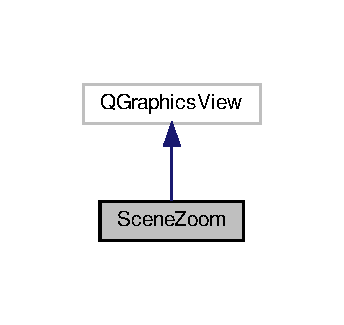
\includegraphics[width=165pt]{classSceneZoom__inherit__graph}
\end{center}
\end{figure}


Граф связей класса Scene\+Zoom\+:\nopagebreak
\begin{figure}[H]
\begin{center}
\leavevmode
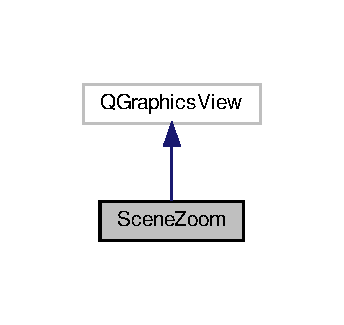
\includegraphics[width=165pt]{classSceneZoom__coll__graph}
\end{center}
\end{figure}
\subsection*{Открытые члены}
\begin{DoxyCompactItemize}
\item 
\hyperlink{classSceneZoom_a4467d1e53eb8d2af1866f25759b0dbcd}{Scene\+Zoom} (Q\+Widget $\ast$parent=nullptr)
\begin{DoxyCompactList}\small\item\em \hyperlink{classSceneZoom}{Scene\+Zoom}. \end{DoxyCompactList}\item 
void \hyperlink{classSceneZoom_a7d535a62dbc00e43b7daabaf6a61f553}{zoom\+In} ()
\begin{DoxyCompactList}\small\item\em zoom\+In \end{DoxyCompactList}\item 
void \hyperlink{classSceneZoom_a9907761406dc1a9f1664429b4004a592}{zoom\+Out} ()
\begin{DoxyCompactList}\small\item\em zoom\+Out \end{DoxyCompactList}\item 
void \hyperlink{classSceneZoom_a6ef95f5202dcc08251417074fbcf14b7}{wheel\+Event} (Q\+Wheel\+Event $\ast$event)
\begin{DoxyCompactList}\small\item\em wheel\+Event \end{DoxyCompactList}\end{DoxyCompactItemize}


\subsection{Подробное описание}
Класс реализующий логику зумирования изображения в сцене на виджете 

\begin{DoxyAuthor}{Автор}
Илья Трефилов 
\end{DoxyAuthor}
\begin{DoxyDate}{Дата}
01.\+12.\+2018
\end{DoxyDate}
Данный класс предназначен для реализации функции зумирования в сценах на виджете 

\subsection{Конструктор(ы)}
\mbox{\Hypertarget{classSceneZoom_a4467d1e53eb8d2af1866f25759b0dbcd}\label{classSceneZoom_a4467d1e53eb8d2af1866f25759b0dbcd}} 
\index{Scene\+Zoom@{Scene\+Zoom}!Scene\+Zoom@{Scene\+Zoom}}
\index{Scene\+Zoom@{Scene\+Zoom}!Scene\+Zoom@{Scene\+Zoom}}
\subsubsection{\texorpdfstring{Scene\+Zoom()}{SceneZoom()}}
{\footnotesize\ttfamily Scene\+Zoom\+::\+Scene\+Zoom (\begin{DoxyParamCaption}\item[{Q\+Widget $\ast$}]{parent = {\ttfamily nullptr} }\end{DoxyParamCaption})}



\hyperlink{classSceneZoom}{Scene\+Zoom}. 


\begin{DoxyParams}{Аргументы}
{\em parent} & Указатель на родительский виджет\\
\hline
\end{DoxyParams}
Конструктор класса сцены с зумированием 

\subsection{Методы}
\mbox{\Hypertarget{classSceneZoom_a6ef95f5202dcc08251417074fbcf14b7}\label{classSceneZoom_a6ef95f5202dcc08251417074fbcf14b7}} 
\index{Scene\+Zoom@{Scene\+Zoom}!wheel\+Event@{wheel\+Event}}
\index{wheel\+Event@{wheel\+Event}!Scene\+Zoom@{Scene\+Zoom}}
\subsubsection{\texorpdfstring{wheel\+Event()}{wheelEvent()}}
{\footnotesize\ttfamily void Scene\+Zoom\+::wheel\+Event (\begin{DoxyParamCaption}\item[{Q\+Wheel\+Event $\ast$}]{event }\end{DoxyParamCaption})}



wheel\+Event 


\begin{DoxyParams}{Аргументы}
{\em event} & Событие прокрутки колеса мыши\\
\hline
\end{DoxyParams}
Функция отлавливает события прокрутки колеса мыши для осуществления зумирования \mbox{\Hypertarget{classSceneZoom_a7d535a62dbc00e43b7daabaf6a61f553}\label{classSceneZoom_a7d535a62dbc00e43b7daabaf6a61f553}} 
\index{Scene\+Zoom@{Scene\+Zoom}!zoom\+In@{zoom\+In}}
\index{zoom\+In@{zoom\+In}!Scene\+Zoom@{Scene\+Zoom}}
\subsubsection{\texorpdfstring{zoom\+In()}{zoomIn()}}
{\footnotesize\ttfamily void Scene\+Zoom\+::zoom\+In (\begin{DoxyParamCaption}{ }\end{DoxyParamCaption})}



zoom\+In 

Функция для увеличения масштаба изображения в сцене \mbox{\Hypertarget{classSceneZoom_a9907761406dc1a9f1664429b4004a592}\label{classSceneZoom_a9907761406dc1a9f1664429b4004a592}} 
\index{Scene\+Zoom@{Scene\+Zoom}!zoom\+Out@{zoom\+Out}}
\index{zoom\+Out@{zoom\+Out}!Scene\+Zoom@{Scene\+Zoom}}
\subsubsection{\texorpdfstring{zoom\+Out()}{zoomOut()}}
{\footnotesize\ttfamily void Scene\+Zoom\+::zoom\+Out (\begin{DoxyParamCaption}{ }\end{DoxyParamCaption})}



zoom\+Out 

Функция для уменьшения масштаба изображения в сцене 

Объявления и описания членов классов находятся в файлах\+:\begin{DoxyCompactItemize}
\item 
\hyperlink{scenezoom_8h}{scenezoom.\+h}\item 
\hyperlink{scenezoom_8cpp}{scenezoom.\+cpp}\end{DoxyCompactItemize}

\hypertarget{classSendDialog}{}\section{Класс Send\+Dialog}
\label{classSendDialog}\index{Send\+Dialog@{Send\+Dialog}}


Класс формы отправки запроса  




{\ttfamily \#include $<$senddialog.\+h$>$}



Граф наследования\+:Send\+Dialog\+:\nopagebreak
\begin{figure}[H]
\begin{center}
\leavevmode
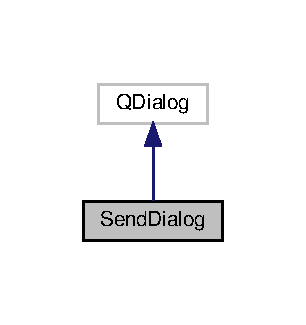
\includegraphics[width=147pt]{classSendDialog__inherit__graph}
\end{center}
\end{figure}


Граф связей класса Send\+Dialog\+:\nopagebreak
\begin{figure}[H]
\begin{center}
\leavevmode
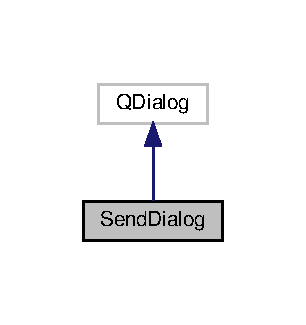
\includegraphics[width=147pt]{classSendDialog__coll__graph}
\end{center}
\end{figure}
\subsection*{Открытые члены}
\begin{DoxyCompactItemize}
\item 
\hyperlink{classSendDialog_a4bfe5b37d110edee9e324c138aaf1377}{Send\+Dialog} (Q\+Widget $\ast$parent=nullptr)
\begin{DoxyCompactList}\small\item\em \hyperlink{classSendDialog}{Send\+Dialog}. \end{DoxyCompactList}\item 
void \hyperlink{classSendDialog_a66420c8a246b7aa3c466087e655ff0ea}{send\+Data} (const Q\+Byte\+Array \&ba, const Q\+String \&host, const int \&id)
\begin{DoxyCompactList}\small\item\em send\+Data \end{DoxyCompactList}\item 
\hyperlink{classSendDialog_af374a7a7ccd8b4dcdd0d567ce72c04a3}{$\sim$\+Send\+Dialog} ()
\end{DoxyCompactItemize}
\subsection*{Закрытые слоты}
\begin{DoxyCompactItemize}
\item 
void \hyperlink{classSendDialog_a542483b8bf0dd1230e060e217d58d468}{on\+\_\+send\+Button\+\_\+clicked} ()
\begin{DoxyCompactList}\small\item\em on\+\_\+send\+Button\+\_\+clicked \end{DoxyCompactList}\end{DoxyCompactItemize}
\subsection*{Закрытые члены}
\begin{DoxyCompactItemize}
\item 
bool \hyperlink{classSendDialog_a479b0de26c1b97fa47ffcbd67252da1f}{init\+Table} ()
\begin{DoxyCompactList}\small\item\em init\+Table \end{DoxyCompactList}\item 
Q\+Json\+Document \hyperlink{classSendDialog_a26dea1897c6af47118f88e89fcc0a7f1}{read\+Config} () const
\begin{DoxyCompactList}\small\item\em read\+Config \end{DoxyCompactList}\item 
\hyperlink{senddialog_8h_aa9b1321518febdee7323e4994ecc1ec3}{id\+With\+Object} \hyperlink{classSendDialog_a7b74a8f29ac1cd411195fb9d9f48cd44}{build\+Tele\+Med\+Object} ()
\begin{DoxyCompactList}\small\item\em build\+Tele\+Med\+Object \end{DoxyCompactList}\item 
bool \hyperlink{classSendDialog_a0bde13a7efe3bd50e9fe67a7b87b9f2c}{connect\+To\+Host} (const Q\+String \&host)
\begin{DoxyCompactList}\small\item\em connect\+To\+Host \end{DoxyCompactList}\item 
bool \hyperlink{classSendDialog_a2942d10e361268fb72c55fa158c57a83}{write\+Data} (const Q\+Byte\+Array \&data)
\begin{DoxyCompactList}\small\item\em write\+Data \end{DoxyCompactList}\item 
Q\+String \hyperlink{classSendDialog_af8fc97ec266db98d488701a4601f1b26}{get\+Host} (const Q\+String \&name) const
\begin{DoxyCompactList}\small\item\em get\+Host \end{DoxyCompactList}\item 
void \hyperlink{classSendDialog_a2bea7a847533969d7a3ff885d6aff656}{update\+Table} (const int \&id, Q\+Byte\+Array \&ba)
\begin{DoxyCompactList}\small\item\em update\+Table \end{DoxyCompactList}\item 
bool \hyperlink{classSendDialog_a6da8a7a2736bad8f3da4d6d8e1608f3d}{build\+Combo\+Box} ()
\begin{DoxyCompactList}\small\item\em build\+Combo\+Box \end{DoxyCompactList}\end{DoxyCompactItemize}
\subsection*{Закрытые данные}
\begin{DoxyCompactItemize}
\item 
Q\+Tcp\+Socket \hyperlink{classSendDialog_a101575f24f58bbbbe03759c3602dcca3}{m\+\_\+tcp\+Socket}
\begin{DoxyCompactList}\small\item\em m\+\_\+tcp\+Socket \end{DoxyCompactList}\item 
Q\+Json\+Document \hyperlink{classSendDialog_a51192da75f8dee9536f99c5b390d858f}{m\+\_\+name\+Mapping}
\begin{DoxyCompactList}\small\item\em m\+\_\+name\+Mapping \end{DoxyCompactList}\item 
Ui\+::\+Send\+Dialog $\ast$ \hyperlink{classSendDialog_af3fd5ba452e7e546ebd1a3160c2333a9}{ui}
\begin{DoxyCompactList}\small\item\em ui \end{DoxyCompactList}\end{DoxyCompactItemize}


\subsection{Подробное описание}
Класс формы отправки запроса 

\begin{DoxyAuthor}{Автор}
Илья Трефилов 
\end{DoxyAuthor}
\begin{DoxyDate}{Дата}
01.\+12.\+2018
\end{DoxyDate}
Класс формы отправки запроса 

\subsection{Конструктор(ы)}
\mbox{\Hypertarget{classSendDialog_a4bfe5b37d110edee9e324c138aaf1377}\label{classSendDialog_a4bfe5b37d110edee9e324c138aaf1377}} 
\index{Send\+Dialog@{Send\+Dialog}!Send\+Dialog@{Send\+Dialog}}
\index{Send\+Dialog@{Send\+Dialog}!Send\+Dialog@{Send\+Dialog}}
\subsubsection{\texorpdfstring{Send\+Dialog()}{SendDialog()}}
{\footnotesize\ttfamily Send\+Dialog\+::\+Send\+Dialog (\begin{DoxyParamCaption}\item[{Q\+Widget $\ast$}]{parent = {\ttfamily nullptr} }\end{DoxyParamCaption})\hspace{0.3cm}{\ttfamily [explicit]}}



\hyperlink{classSendDialog}{Send\+Dialog}. 


\begin{DoxyParams}{Аргументы}
{\em parent} & Указатель на родительский виджет\\
\hline
\end{DoxyParams}
Конструктор класса формы \mbox{\Hypertarget{classSendDialog_af374a7a7ccd8b4dcdd0d567ce72c04a3}\label{classSendDialog_af374a7a7ccd8b4dcdd0d567ce72c04a3}} 
\index{Send\+Dialog@{Send\+Dialog}!````~Send\+Dialog@{$\sim$\+Send\+Dialog}}
\index{````~Send\+Dialog@{$\sim$\+Send\+Dialog}!Send\+Dialog@{Send\+Dialog}}
\subsubsection{\texorpdfstring{$\sim$\+Send\+Dialog()}{~SendDialog()}}
{\footnotesize\ttfamily Send\+Dialog\+::$\sim$\+Send\+Dialog (\begin{DoxyParamCaption}{ }\end{DoxyParamCaption})}



\subsection{Методы}
\mbox{\Hypertarget{classSendDialog_a6da8a7a2736bad8f3da4d6d8e1608f3d}\label{classSendDialog_a6da8a7a2736bad8f3da4d6d8e1608f3d}} 
\index{Send\+Dialog@{Send\+Dialog}!build\+Combo\+Box@{build\+Combo\+Box}}
\index{build\+Combo\+Box@{build\+Combo\+Box}!Send\+Dialog@{Send\+Dialog}}
\subsubsection{\texorpdfstring{build\+Combo\+Box()}{buildComboBox()}}
{\footnotesize\ttfamily bool Send\+Dialog\+::build\+Combo\+Box (\begin{DoxyParamCaption}{ }\end{DoxyParamCaption})\hspace{0.3cm}{\ttfamily [private]}}



build\+Combo\+Box 

\begin{DoxyReturn}{Возвращает}
true -\/ если удалось получить имена из файла config.\+json для их отображения в боксе
\end{DoxyReturn}
Функция строит бокс с выпадающим списком с именами врачей для отправки данных Имя отображается на ip адрес \mbox{\Hypertarget{classSendDialog_a7b74a8f29ac1cd411195fb9d9f48cd44}\label{classSendDialog_a7b74a8f29ac1cd411195fb9d9f48cd44}} 
\index{Send\+Dialog@{Send\+Dialog}!build\+Tele\+Med\+Object@{build\+Tele\+Med\+Object}}
\index{build\+Tele\+Med\+Object@{build\+Tele\+Med\+Object}!Send\+Dialog@{Send\+Dialog}}
\subsubsection{\texorpdfstring{build\+Tele\+Med\+Object()}{buildTeleMedObject()}}
{\footnotesize\ttfamily \hyperlink{senddialog_8h_aa9b1321518febdee7323e4994ecc1ec3}{id\+With\+Object} Send\+Dialog\+::build\+Tele\+Med\+Object (\begin{DoxyParamCaption}{ }\end{DoxyParamCaption})\hspace{0.3cm}{\ttfamily [private]}}



build\+Tele\+Med\+Object 

\begin{DoxyReturn}{Возвращает}
Объект -\/ пару, информация о отправляемом объекте и id из базы данных
\end{DoxyReturn}
Функция для построения объекта, связующего информацию в запросе и номер объекта в базе данных \mbox{\Hypertarget{classSendDialog_a0bde13a7efe3bd50e9fe67a7b87b9f2c}\label{classSendDialog_a0bde13a7efe3bd50e9fe67a7b87b9f2c}} 
\index{Send\+Dialog@{Send\+Dialog}!connect\+To\+Host@{connect\+To\+Host}}
\index{connect\+To\+Host@{connect\+To\+Host}!Send\+Dialog@{Send\+Dialog}}
\subsubsection{\texorpdfstring{connect\+To\+Host()}{connectToHost()}}
{\footnotesize\ttfamily bool Send\+Dialog\+::connect\+To\+Host (\begin{DoxyParamCaption}\item[{const Q\+String \&}]{host }\end{DoxyParamCaption})\hspace{0.3cm}{\ttfamily [private]}}



connect\+To\+Host 


\begin{DoxyParams}{Аргументы}
{\em host} & ip адрес или имя хоста в сети, куда надо отправить данные \\
\hline
\end{DoxyParams}
\begin{DoxyReturn}{Возвращает}
true -\/ если подключение было успешным
\end{DoxyReturn}
Функция для подключения к принимающему информацию хосту \mbox{\Hypertarget{classSendDialog_af8fc97ec266db98d488701a4601f1b26}\label{classSendDialog_af8fc97ec266db98d488701a4601f1b26}} 
\index{Send\+Dialog@{Send\+Dialog}!get\+Host@{get\+Host}}
\index{get\+Host@{get\+Host}!Send\+Dialog@{Send\+Dialog}}
\subsubsection{\texorpdfstring{get\+Host()}{getHost()}}
{\footnotesize\ttfamily Q\+String Send\+Dialog\+::get\+Host (\begin{DoxyParamCaption}\item[{const Q\+String \&}]{name }\end{DoxyParamCaption}) const\hspace{0.3cm}{\ttfamily [private]}}



get\+Host 


\begin{DoxyParams}{Аргументы}
{\em name} & Имя врача \\
\hline
\end{DoxyParams}
\begin{DoxyReturn}{Возвращает}
Ip адрес или имя хоста в сети выбранного врача
\end{DoxyReturn}
Функция для получения ip адреса по имени \mbox{\Hypertarget{classSendDialog_a479b0de26c1b97fa47ffcbd67252da1f}\label{classSendDialog_a479b0de26c1b97fa47ffcbd67252da1f}} 
\index{Send\+Dialog@{Send\+Dialog}!init\+Table@{init\+Table}}
\index{init\+Table@{init\+Table}!Send\+Dialog@{Send\+Dialog}}
\subsubsection{\texorpdfstring{init\+Table()}{initTable()}}
{\footnotesize\ttfamily bool Send\+Dialog\+::init\+Table (\begin{DoxyParamCaption}{ }\end{DoxyParamCaption})\hspace{0.3cm}{\ttfamily [private]}}



init\+Table 

\begin{DoxyReturn}{Возвращает}
true -\/ если удалось получить данные из таблицы базы данных в таблицу виджета
\end{DoxyReturn}
Функция инициализирующая таблицу с информацией из базы данных \mbox{\Hypertarget{classSendDialog_a542483b8bf0dd1230e060e217d58d468}\label{classSendDialog_a542483b8bf0dd1230e060e217d58d468}} 
\index{Send\+Dialog@{Send\+Dialog}!on\+\_\+send\+Button\+\_\+clicked@{on\+\_\+send\+Button\+\_\+clicked}}
\index{on\+\_\+send\+Button\+\_\+clicked@{on\+\_\+send\+Button\+\_\+clicked}!Send\+Dialog@{Send\+Dialog}}
\subsubsection{\texorpdfstring{on\+\_\+send\+Button\+\_\+clicked}{on\_sendButton\_clicked}}
{\footnotesize\ttfamily void Send\+Dialog\+::on\+\_\+send\+Button\+\_\+clicked (\begin{DoxyParamCaption}{ }\end{DoxyParamCaption})\hspace{0.3cm}{\ttfamily [private]}, {\ttfamily [slot]}}



on\+\_\+send\+Button\+\_\+clicked 

Слот принимающий нажатие на кнопку отправить и отправляющий данные. Проверки на валидность ввода реализованы \mbox{\Hypertarget{classSendDialog_a26dea1897c6af47118f88e89fcc0a7f1}\label{classSendDialog_a26dea1897c6af47118f88e89fcc0a7f1}} 
\index{Send\+Dialog@{Send\+Dialog}!read\+Config@{read\+Config}}
\index{read\+Config@{read\+Config}!Send\+Dialog@{Send\+Dialog}}
\subsubsection{\texorpdfstring{read\+Config()}{readConfig()}}
{\footnotesize\ttfamily Q\+Json\+Document Send\+Dialog\+::read\+Config (\begin{DoxyParamCaption}{ }\end{DoxyParamCaption}) const\hspace{0.3cm}{\ttfamily [private]}}



read\+Config 

\begin{DoxyReturn}{Возвращает}
Объект, представляющий json из файла
\end{DoxyReturn}
Функция читающая файл config.\+json, возвращает объет типа J\+S\+ON из данного файла Данная функция необходима для отображения ip адресов на имена врачей \mbox{\Hypertarget{classSendDialog_a66420c8a246b7aa3c466087e655ff0ea}\label{classSendDialog_a66420c8a246b7aa3c466087e655ff0ea}} 
\index{Send\+Dialog@{Send\+Dialog}!send\+Data@{send\+Data}}
\index{send\+Data@{send\+Data}!Send\+Dialog@{Send\+Dialog}}
\subsubsection{\texorpdfstring{send\+Data()}{sendData()}}
{\footnotesize\ttfamily void Send\+Dialog\+::send\+Data (\begin{DoxyParamCaption}\item[{const Q\+Byte\+Array \&}]{ba,  }\item[{const Q\+String \&}]{host,  }\item[{const int \&}]{id }\end{DoxyParamCaption})}



send\+Data 


\begin{DoxyParams}{Аргументы}
{\em ba} & Набор байт для отправки по сети \\
\hline
{\em host} & Ip адресс или имя хоста на который надо отправить информацию \\
\hline
{\em id} & Номер объекта из базы данных для отправки\\
\hline
\end{DoxyParams}
Функция отправляет объект информации о клиента из базы данных в виде бинарных данных по сети \mbox{\Hypertarget{classSendDialog_a2bea7a847533969d7a3ff885d6aff656}\label{classSendDialog_a2bea7a847533969d7a3ff885d6aff656}} 
\index{Send\+Dialog@{Send\+Dialog}!update\+Table@{update\+Table}}
\index{update\+Table@{update\+Table}!Send\+Dialog@{Send\+Dialog}}
\subsubsection{\texorpdfstring{update\+Table()}{updateTable()}}
{\footnotesize\ttfamily void Send\+Dialog\+::update\+Table (\begin{DoxyParamCaption}\item[{const int \&}]{id,  }\item[{Q\+Byte\+Array \&}]{ba }\end{DoxyParamCaption})\hspace{0.3cm}{\ttfamily [private]}}



update\+Table 


\begin{DoxyParams}{Аргументы}
{\em id} & Номер отправляемого объекта в базе данных \\
\hline
{\em ba} & Бинарные данные, представлюящие объект запроса\\
\hline
\end{DoxyParams}
Функция обновляет данные в таблице базы данных после отправки запроса \mbox{\Hypertarget{classSendDialog_a2942d10e361268fb72c55fa158c57a83}\label{classSendDialog_a2942d10e361268fb72c55fa158c57a83}} 
\index{Send\+Dialog@{Send\+Dialog}!write\+Data@{write\+Data}}
\index{write\+Data@{write\+Data}!Send\+Dialog@{Send\+Dialog}}
\subsubsection{\texorpdfstring{write\+Data()}{writeData()}}
{\footnotesize\ttfamily bool Send\+Dialog\+::write\+Data (\begin{DoxyParamCaption}\item[{const Q\+Byte\+Array \&}]{data }\end{DoxyParamCaption})\hspace{0.3cm}{\ttfamily [private]}}



write\+Data 


\begin{DoxyParams}{Аргументы}
{\em data} & Бинарные данные, представлюящие объект запроса \\
\hline
\end{DoxyParams}
\begin{DoxyReturn}{Возвращает}
true -\/ если запись была успешна
\end{DoxyReturn}
Записывает данные в открытое соединение между отправляющей и принимающей стороной 

\subsection{Данные класса}
\mbox{\Hypertarget{classSendDialog_a51192da75f8dee9536f99c5b390d858f}\label{classSendDialog_a51192da75f8dee9536f99c5b390d858f}} 
\index{Send\+Dialog@{Send\+Dialog}!m\+\_\+name\+Mapping@{m\+\_\+name\+Mapping}}
\index{m\+\_\+name\+Mapping@{m\+\_\+name\+Mapping}!Send\+Dialog@{Send\+Dialog}}
\subsubsection{\texorpdfstring{m\+\_\+name\+Mapping}{m\_nameMapping}}
{\footnotesize\ttfamily Q\+Json\+Document Send\+Dialog\+::m\+\_\+name\+Mapping\hspace{0.3cm}{\ttfamily [private]}}



m\+\_\+name\+Mapping 

Объект, представляющий докумет типа J\+S\+ON \mbox{\Hypertarget{classSendDialog_a101575f24f58bbbbe03759c3602dcca3}\label{classSendDialog_a101575f24f58bbbbe03759c3602dcca3}} 
\index{Send\+Dialog@{Send\+Dialog}!m\+\_\+tcp\+Socket@{m\+\_\+tcp\+Socket}}
\index{m\+\_\+tcp\+Socket@{m\+\_\+tcp\+Socket}!Send\+Dialog@{Send\+Dialog}}
\subsubsection{\texorpdfstring{m\+\_\+tcp\+Socket}{m\_tcpSocket}}
{\footnotesize\ttfamily Q\+Tcp\+Socket Send\+Dialog\+::m\+\_\+tcp\+Socket\hspace{0.3cm}{\ttfamily [private]}}



m\+\_\+tcp\+Socket 

Сокет для отправки данных по сети \mbox{\Hypertarget{classSendDialog_af3fd5ba452e7e546ebd1a3160c2333a9}\label{classSendDialog_af3fd5ba452e7e546ebd1a3160c2333a9}} 
\index{Send\+Dialog@{Send\+Dialog}!ui@{ui}}
\index{ui@{ui}!Send\+Dialog@{Send\+Dialog}}
\subsubsection{\texorpdfstring{ui}{ui}}
{\footnotesize\ttfamily Ui\+::\+Send\+Dialog$\ast$ Send\+Dialog\+::ui\hspace{0.3cm}{\ttfamily [private]}}



ui 

Указатель на объект интерфейса для формы отправки данных 

Объявления и описания членов классов находятся в файлах\+:\begin{DoxyCompactItemize}
\item 
\hyperlink{senddialog_8h}{senddialog.\+h}\item 
\hyperlink{senddialog_8cpp}{senddialog.\+cpp}\end{DoxyCompactItemize}

\hypertarget{classServer}{}\section{Класс Server}
\label{classServer}\index{Server@{Server}}


Класс сервера  




{\ttfamily \#include $<$server.\+h$>$}



Граф наследования\+:Server\+:\nopagebreak
\begin{figure}[H]
\begin{center}
\leavevmode
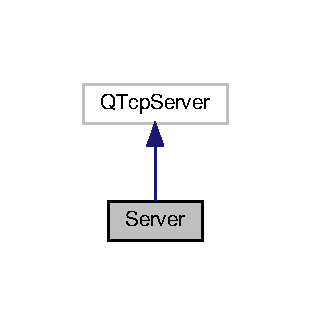
\includegraphics[width=149pt]{classServer__inherit__graph}
\end{center}
\end{figure}


Граф связей класса Server\+:\nopagebreak
\begin{figure}[H]
\begin{center}
\leavevmode
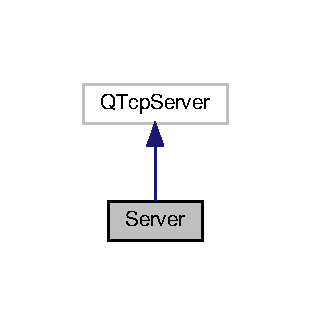
\includegraphics[width=149pt]{classServer__coll__graph}
\end{center}
\end{figure}
\subsection*{Открытые слоты}
\begin{DoxyCompactItemize}
\item 
void \hyperlink{classServer_a9ef1fd70a951bc612605f87b4540b308}{Get\+Data\+From\+Client} (Q\+Byte\+Array ba)
\begin{DoxyCompactList}\small\item\em Get\+Data\+From\+Client. \end{DoxyCompactList}\end{DoxyCompactItemize}
\subsection*{Сигналы}
\begin{DoxyCompactItemize}
\item 
void \hyperlink{classServer_a3fddab101fd0c1b85570209fcad7155c}{transfer\+Data\+To\+Widget} (Q\+Byte\+Array ba)
\begin{DoxyCompactList}\small\item\em transfer\+Data\+To\+Widget \end{DoxyCompactList}\end{DoxyCompactItemize}
\subsection*{Открытые члены}
\begin{DoxyCompactItemize}
\item 
\hyperlink{classServer_aaf98d5194faee831c6340cc736b9b879}{Server} (Q\+Object $\ast$parent=nullptr)
\begin{DoxyCompactList}\small\item\em \hyperlink{classServer}{Server}. \end{DoxyCompactList}\item 
void \hyperlink{classServer_af59bb3a96b3311ed2b87e2d6899d9f79}{start\+Server} ()
\begin{DoxyCompactList}\small\item\em start\+Server \end{DoxyCompactList}\end{DoxyCompactItemize}
\subsection*{Защищенные члены}
\begin{DoxyCompactItemize}
\item 
void \hyperlink{classServer_a3952d37b7bc53a4377f411d9ccaa9d62}{incoming\+Connection} (qintptr socket\+Descriptor)
\begin{DoxyCompactList}\small\item\em incoming\+Connection \end{DoxyCompactList}\end{DoxyCompactItemize}


\subsection{Подробное описание}
Класс сервера 

\begin{DoxyAuthor}{Автор}
Илья Трефилов 
\end{DoxyAuthor}
\begin{DoxyDate}{Дата}
01.\+12.\+2018
\end{DoxyDate}
Класс сервера для приема запросов 

\subsection{Конструктор(ы)}
\mbox{\Hypertarget{classServer_aaf98d5194faee831c6340cc736b9b879}\label{classServer_aaf98d5194faee831c6340cc736b9b879}} 
\index{Server@{Server}!Server@{Server}}
\index{Server@{Server}!Server@{Server}}
\subsubsection{\texorpdfstring{Server()}{Server()}}
{\footnotesize\ttfamily Server\+::\+Server (\begin{DoxyParamCaption}\item[{Q\+Object $\ast$}]{parent = {\ttfamily nullptr} }\end{DoxyParamCaption})\hspace{0.3cm}{\ttfamily [explicit]}}



\hyperlink{classServer}{Server}. 


\begin{DoxyParams}{Аргументы}
{\em parent} & Указатель на родительский объект\\
\hline
\end{DoxyParams}
Конструктор класса сервера 

\subsection{Методы}
\mbox{\Hypertarget{classServer_a9ef1fd70a951bc612605f87b4540b308}\label{classServer_a9ef1fd70a951bc612605f87b4540b308}} 
\index{Server@{Server}!Get\+Data\+From\+Client@{Get\+Data\+From\+Client}}
\index{Get\+Data\+From\+Client@{Get\+Data\+From\+Client}!Server@{Server}}
\subsubsection{\texorpdfstring{Get\+Data\+From\+Client}{GetDataFromClient}}
{\footnotesize\ttfamily void Server\+::\+Get\+Data\+From\+Client (\begin{DoxyParamCaption}\item[{Q\+Byte\+Array}]{ba }\end{DoxyParamCaption})\hspace{0.3cm}{\ttfamily [slot]}}



Get\+Data\+From\+Client. 


\begin{DoxyParams}{Аргументы}
{\em ba} & Набор байт\\
\hline
\end{DoxyParams}
Слот для получения информации от потока обрабатывающего соединение \mbox{\Hypertarget{classServer_a3952d37b7bc53a4377f411d9ccaa9d62}\label{classServer_a3952d37b7bc53a4377f411d9ccaa9d62}} 
\index{Server@{Server}!incoming\+Connection@{incoming\+Connection}}
\index{incoming\+Connection@{incoming\+Connection}!Server@{Server}}
\subsubsection{\texorpdfstring{incoming\+Connection()}{incomingConnection()}}
{\footnotesize\ttfamily void Server\+::incoming\+Connection (\begin{DoxyParamCaption}\item[{qintptr}]{socket\+Descriptor }\end{DoxyParamCaption})\hspace{0.3cm}{\ttfamily [protected]}}



incoming\+Connection 


\begin{DoxyParams}{Аргументы}
{\em socket\+Descriptor} & Дескриптор сокета при соединении\\
\hline
\end{DoxyParams}
Функция для обработки входящего соединения и выделения необходимых системных ресурсов \mbox{\Hypertarget{classServer_af59bb3a96b3311ed2b87e2d6899d9f79}\label{classServer_af59bb3a96b3311ed2b87e2d6899d9f79}} 
\index{Server@{Server}!start\+Server@{start\+Server}}
\index{start\+Server@{start\+Server}!Server@{Server}}
\subsubsection{\texorpdfstring{start\+Server()}{startServer()}}
{\footnotesize\ttfamily void Server\+::start\+Server (\begin{DoxyParamCaption}{ }\end{DoxyParamCaption})}



start\+Server 

Функция для запуска сервера на порту 7808 \mbox{\Hypertarget{classServer_a3fddab101fd0c1b85570209fcad7155c}\label{classServer_a3fddab101fd0c1b85570209fcad7155c}} 
\index{Server@{Server}!transfer\+Data\+To\+Widget@{transfer\+Data\+To\+Widget}}
\index{transfer\+Data\+To\+Widget@{transfer\+Data\+To\+Widget}!Server@{Server}}
\subsubsection{\texorpdfstring{transfer\+Data\+To\+Widget}{transferDataToWidget}}
{\footnotesize\ttfamily void Server\+::transfer\+Data\+To\+Widget (\begin{DoxyParamCaption}\item[{Q\+Byte\+Array}]{ba }\end{DoxyParamCaption})\hspace{0.3cm}{\ttfamily [signal]}}



transfer\+Data\+To\+Widget 


\begin{DoxyParams}{Аргументы}
{\em ba} & Набор байт\\
\hline
\end{DoxyParams}
Сигнал для передачи полученной информации в класс виджет для отображения 

Объявления и описания членов классов находятся в файлах\+:\begin{DoxyCompactItemize}
\item 
\hyperlink{server_8h}{server.\+h}\item 
\hyperlink{server_8cpp}{server.\+cpp}\end{DoxyCompactItemize}

\hypertarget{classSideBar}{}\section{Класс Side\+Bar}
\label{classSideBar}\index{Side\+Bar@{Side\+Bar}}


Класс формы боковой панели выбора виджета  




{\ttfamily \#include $<$sidebar.\+h$>$}



Граф наследования\+:Side\+Bar\+:\nopagebreak
\begin{figure}[H]
\begin{center}
\leavevmode
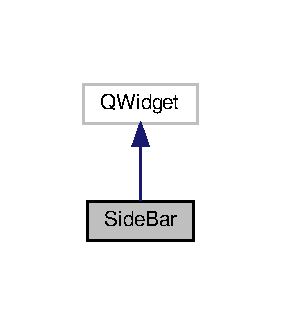
\includegraphics[width=135pt]{classSideBar__inherit__graph}
\end{center}
\end{figure}


Граф связей класса Side\+Bar\+:\nopagebreak
\begin{figure}[H]
\begin{center}
\leavevmode
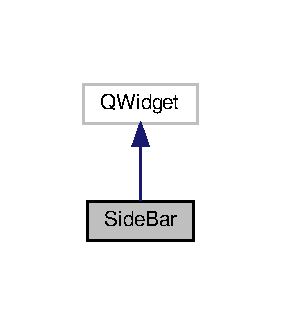
\includegraphics[width=135pt]{classSideBar__coll__graph}
\end{center}
\end{figure}
\subsection*{Открытые члены}
\begin{DoxyCompactItemize}
\item 
\hyperlink{classSideBar_a2a5215a713fe300f8e7b2407017db411}{Side\+Bar} (Q\+Widget $\ast$parent=nullptr)
\begin{DoxyCompactList}\small\item\em \hyperlink{classSideBar}{Side\+Bar}. \end{DoxyCompactList}\item 
void \hyperlink{classSideBar_abec6727f29e75af996bc71196c690eaa}{add\+Action} (Q\+Action $\ast$action)
\begin{DoxyCompactList}\small\item\em add\+Action \end{DoxyCompactList}\item 
Q\+Action $\ast$ \hyperlink{classSideBar_abcc7410af74a6e776a4d708a396f47ec}{add\+Action} (const Q\+String \&text, const Q\+Icon \&icon=Q\+Icon())
\begin{DoxyCompactList}\small\item\em add\+Action \end{DoxyCompactList}\item 
Q\+Size \hyperlink{classSideBar_a3b46466ef84c9f89677478f8b1f5bf36}{minimum\+Size\+Hint} () const
\begin{DoxyCompactList}\small\item\em minimum\+Size\+Hint \end{DoxyCompactList}\end{DoxyCompactItemize}
\subsection*{Защищенные члены}
\begin{DoxyCompactItemize}
\item 
void \hyperlink{classSideBar_a99c8319ee78b2197db5eda7b2cd232a1}{paint\+Event} (Q\+Paint\+Event $\ast$event)
\begin{DoxyCompactList}\small\item\em paint\+Event \end{DoxyCompactList}\item 
void \hyperlink{classSideBar_ae3923b2d85345b3f7b899ce6becd21fb}{mouse\+Press\+Event} (Q\+Mouse\+Event $\ast$event)
\begin{DoxyCompactList}\small\item\em mouse\+Press\+Event \end{DoxyCompactList}\item 
void \hyperlink{classSideBar_a1c00fa33ba20510bf7d50dfa757a8515}{mouse\+Move\+Event} (Q\+Mouse\+Event $\ast$event)
\begin{DoxyCompactList}\small\item\em mouse\+Move\+Event \end{DoxyCompactList}\item 
void \hyperlink{classSideBar_a123dcd87817fecdfacd60fd967044908}{leave\+Event} (Q\+Event $\ast$event)
\begin{DoxyCompactList}\small\item\em leave\+Event \end{DoxyCompactList}\item 
Q\+Action $\ast$ \hyperlink{classSideBar_a003659c2c40670c3f2bb31798ff87c3d}{action\+At} (const Q\+Point \&at)
\begin{DoxyCompactList}\small\item\em action\+At \end{DoxyCompactList}\end{DoxyCompactItemize}
\subsection*{Закрытые данные}
\begin{DoxyCompactItemize}
\item 
Q\+List$<$ Q\+Action $\ast$ $>$ \hyperlink{classSideBar_aeb09886c01726197d79d417ce22322d4}{m\+Actions}
\begin{DoxyCompactList}\small\item\em m\+Actions \end{DoxyCompactList}\item 
Q\+Action $\ast$ \hyperlink{classSideBar_a2db27c5981c8f43be372af9bbbe8fa41}{m\+Checked\+Action}
\begin{DoxyCompactList}\small\item\em m\+Checked\+Action \end{DoxyCompactList}\item 
Q\+Action $\ast$ \hyperlink{classSideBar_a51fcdf6ce60fba976982b2ef06bec853}{m\+Over\+Action}
\begin{DoxyCompactList}\small\item\em m\+Over\+Action \end{DoxyCompactList}\end{DoxyCompactItemize}


\subsection{Подробное описание}
Класс формы боковой панели выбора виджета 

\begin{DoxyAuthor}{Автор}
Илья Трефилов 
\end{DoxyAuthor}
\begin{DoxyDate}{Дата}
01.\+12.\+2018
\end{DoxyDate}
Класс формы боковой панели выбора виджета 

\subsection{Конструктор(ы)}
\mbox{\Hypertarget{classSideBar_a2a5215a713fe300f8e7b2407017db411}\label{classSideBar_a2a5215a713fe300f8e7b2407017db411}} 
\index{Side\+Bar@{Side\+Bar}!Side\+Bar@{Side\+Bar}}
\index{Side\+Bar@{Side\+Bar}!Side\+Bar@{Side\+Bar}}
\subsubsection{\texorpdfstring{Side\+Bar()}{SideBar()}}
{\footnotesize\ttfamily Side\+Bar\+::\+Side\+Bar (\begin{DoxyParamCaption}\item[{Q\+Widget $\ast$}]{parent = {\ttfamily nullptr} }\end{DoxyParamCaption})\hspace{0.3cm}{\ttfamily [explicit]}}



\hyperlink{classSideBar}{Side\+Bar}. 


\begin{DoxyParams}{Аргументы}
{\em parent} & Указатель на родительский виджет\\
\hline
\end{DoxyParams}
Конструктор класса боковой панели 

\subsection{Методы}
\mbox{\Hypertarget{classSideBar_a003659c2c40670c3f2bb31798ff87c3d}\label{classSideBar_a003659c2c40670c3f2bb31798ff87c3d}} 
\index{Side\+Bar@{Side\+Bar}!action\+At@{action\+At}}
\index{action\+At@{action\+At}!Side\+Bar@{Side\+Bar}}
\subsubsection{\texorpdfstring{action\+At()}{actionAt()}}
{\footnotesize\ttfamily Q\+Action $\ast$ Side\+Bar\+::action\+At (\begin{DoxyParamCaption}\item[{const Q\+Point \&}]{at }\end{DoxyParamCaption})\hspace{0.3cm}{\ttfamily [protected]}}



action\+At 


\begin{DoxyParams}{Аргументы}
{\em at} & Координаты расположения курсора \\
\hline
\end{DoxyParams}
\begin{DoxyReturn}{Возвращает}
Объект действия при нажатии на выбранный виджет
\end{DoxyReturn}
Функция возвращающая объект поля по заданным координатам \mbox{\Hypertarget{classSideBar_abec6727f29e75af996bc71196c690eaa}\label{classSideBar_abec6727f29e75af996bc71196c690eaa}} 
\index{Side\+Bar@{Side\+Bar}!add\+Action@{add\+Action}}
\index{add\+Action@{add\+Action}!Side\+Bar@{Side\+Bar}}
\subsubsection{\texorpdfstring{add\+Action()}{addAction()}\hspace{0.1cm}{\footnotesize\ttfamily [1/2]}}
{\footnotesize\ttfamily void Side\+Bar\+::add\+Action (\begin{DoxyParamCaption}\item[{Q\+Action $\ast$}]{action }\end{DoxyParamCaption})}



add\+Action 


\begin{DoxyParams}{Аргументы}
{\em action} & Объект действия при нажатии на выбранный виджет\\
\hline
\end{DoxyParams}
Функция добавляет поле в боковую панель \mbox{\Hypertarget{classSideBar_abcc7410af74a6e776a4d708a396f47ec}\label{classSideBar_abcc7410af74a6e776a4d708a396f47ec}} 
\index{Side\+Bar@{Side\+Bar}!add\+Action@{add\+Action}}
\index{add\+Action@{add\+Action}!Side\+Bar@{Side\+Bar}}
\subsubsection{\texorpdfstring{add\+Action()}{addAction()}\hspace{0.1cm}{\footnotesize\ttfamily [2/2]}}
{\footnotesize\ttfamily Q\+Action $\ast$ Side\+Bar\+::add\+Action (\begin{DoxyParamCaption}\item[{const Q\+String \&}]{text,  }\item[{const Q\+Icon \&}]{icon = {\ttfamily QIcon()} }\end{DoxyParamCaption})}



add\+Action 


\begin{DoxyParams}{Аргументы}
{\em text} & Текст в поле боковой панели \\
\hline
{\em icon} & Иконка в поле боковой панели \\
\hline
\end{DoxyParams}
\begin{DoxyReturn}{Возвращает}
Объект действия при нажатии на выбранный виджет 
\end{DoxyReturn}
\mbox{\Hypertarget{classSideBar_a123dcd87817fecdfacd60fd967044908}\label{classSideBar_a123dcd87817fecdfacd60fd967044908}} 
\index{Side\+Bar@{Side\+Bar}!leave\+Event@{leave\+Event}}
\index{leave\+Event@{leave\+Event}!Side\+Bar@{Side\+Bar}}
\subsubsection{\texorpdfstring{leave\+Event()}{leaveEvent()}}
{\footnotesize\ttfamily void Side\+Bar\+::leave\+Event (\begin{DoxyParamCaption}\item[{Q\+Event $\ast$}]{event }\end{DoxyParamCaption})\hspace{0.3cm}{\ttfamily [protected]}}



leave\+Event 


\begin{DoxyParams}{Аргументы}
{\em event} & Событие увода курсора с поля\\
\hline
\end{DoxyParams}
Событие отменяет подсветку, если курсор больше не находится на выбранном поле \mbox{\Hypertarget{classSideBar_a3b46466ef84c9f89677478f8b1f5bf36}\label{classSideBar_a3b46466ef84c9f89677478f8b1f5bf36}} 
\index{Side\+Bar@{Side\+Bar}!minimum\+Size\+Hint@{minimum\+Size\+Hint}}
\index{minimum\+Size\+Hint@{minimum\+Size\+Hint}!Side\+Bar@{Side\+Bar}}
\subsubsection{\texorpdfstring{minimum\+Size\+Hint()}{minimumSizeHint()}}
{\footnotesize\ttfamily Q\+Size Side\+Bar\+::minimum\+Size\+Hint (\begin{DoxyParamCaption}{ }\end{DoxyParamCaption}) const}



minimum\+Size\+Hint 

\begin{DoxyReturn}{Возвращает}
Размер поля
\end{DoxyReturn}
Функция для получения валидного размера поля в боковой панели \mbox{\Hypertarget{classSideBar_a1c00fa33ba20510bf7d50dfa757a8515}\label{classSideBar_a1c00fa33ba20510bf7d50dfa757a8515}} 
\index{Side\+Bar@{Side\+Bar}!mouse\+Move\+Event@{mouse\+Move\+Event}}
\index{mouse\+Move\+Event@{mouse\+Move\+Event}!Side\+Bar@{Side\+Bar}}
\subsubsection{\texorpdfstring{mouse\+Move\+Event()}{mouseMoveEvent()}}
{\footnotesize\ttfamily void Side\+Bar\+::mouse\+Move\+Event (\begin{DoxyParamCaption}\item[{Q\+Mouse\+Event $\ast$}]{event }\end{DoxyParamCaption})\hspace{0.3cm}{\ttfamily [protected]}}



mouse\+Move\+Event 


\begin{DoxyParams}{Аргументы}
{\em event} & Событие наведение мыши\\
\hline
\end{DoxyParams}
Событие подсвечивает поле, на котором расположен курсор \mbox{\Hypertarget{classSideBar_ae3923b2d85345b3f7b899ce6becd21fb}\label{classSideBar_ae3923b2d85345b3f7b899ce6becd21fb}} 
\index{Side\+Bar@{Side\+Bar}!mouse\+Press\+Event@{mouse\+Press\+Event}}
\index{mouse\+Press\+Event@{mouse\+Press\+Event}!Side\+Bar@{Side\+Bar}}
\subsubsection{\texorpdfstring{mouse\+Press\+Event()}{mousePressEvent()}}
{\footnotesize\ttfamily void Side\+Bar\+::mouse\+Press\+Event (\begin{DoxyParamCaption}\item[{Q\+Mouse\+Event $\ast$}]{event }\end{DoxyParamCaption})\hspace{0.3cm}{\ttfamily [protected]}}



mouse\+Press\+Event 


\begin{DoxyParams}{Аргументы}
{\em event} & Событие нажатия мыши\\
\hline
\end{DoxyParams}
Событие при нажатии кнопкой мыши на поле, посылает сигнал в главное окно для отображения выбранного виджета \mbox{\Hypertarget{classSideBar_a99c8319ee78b2197db5eda7b2cd232a1}\label{classSideBar_a99c8319ee78b2197db5eda7b2cd232a1}} 
\index{Side\+Bar@{Side\+Bar}!paint\+Event@{paint\+Event}}
\index{paint\+Event@{paint\+Event}!Side\+Bar@{Side\+Bar}}
\subsubsection{\texorpdfstring{paint\+Event()}{paintEvent()}}
{\footnotesize\ttfamily void Side\+Bar\+::paint\+Event (\begin{DoxyParamCaption}\item[{Q\+Paint\+Event $\ast$}]{event }\end{DoxyParamCaption})\hspace{0.3cm}{\ttfamily [protected]}}



paint\+Event 


\begin{DoxyParams}{Аргументы}
{\em event} & Событие отрисовки\\
\hline
\end{DoxyParams}
Событие для отрисовки поля в боковой панели при его добавлении 

\subsection{Данные класса}
\mbox{\Hypertarget{classSideBar_aeb09886c01726197d79d417ce22322d4}\label{classSideBar_aeb09886c01726197d79d417ce22322d4}} 
\index{Side\+Bar@{Side\+Bar}!m\+Actions@{m\+Actions}}
\index{m\+Actions@{m\+Actions}!Side\+Bar@{Side\+Bar}}
\subsubsection{\texorpdfstring{m\+Actions}{mActions}}
{\footnotesize\ttfamily Q\+List$<$Q\+Action $\ast$$>$ Side\+Bar\+::m\+Actions\hspace{0.3cm}{\ttfamily [private]}}



m\+Actions 

Список полей в боковой панели \mbox{\Hypertarget{classSideBar_a2db27c5981c8f43be372af9bbbe8fa41}\label{classSideBar_a2db27c5981c8f43be372af9bbbe8fa41}} 
\index{Side\+Bar@{Side\+Bar}!m\+Checked\+Action@{m\+Checked\+Action}}
\index{m\+Checked\+Action@{m\+Checked\+Action}!Side\+Bar@{Side\+Bar}}
\subsubsection{\texorpdfstring{m\+Checked\+Action}{mCheckedAction}}
{\footnotesize\ttfamily Q\+Action$\ast$ Side\+Bar\+::m\+Checked\+Action\hspace{0.3cm}{\ttfamily [private]}}



m\+Checked\+Action 

Выбранное поле \mbox{\Hypertarget{classSideBar_a51fcdf6ce60fba976982b2ef06bec853}\label{classSideBar_a51fcdf6ce60fba976982b2ef06bec853}} 
\index{Side\+Bar@{Side\+Bar}!m\+Over\+Action@{m\+Over\+Action}}
\index{m\+Over\+Action@{m\+Over\+Action}!Side\+Bar@{Side\+Bar}}
\subsubsection{\texorpdfstring{m\+Over\+Action}{mOverAction}}
{\footnotesize\ttfamily Q\+Action$\ast$ Side\+Bar\+::m\+Over\+Action\hspace{0.3cm}{\ttfamily [private]}}



m\+Over\+Action 

Поле на котором расположен курсор 

Объявления и описания членов классов находятся в файлах\+:\begin{DoxyCompactItemize}
\item 
\hyperlink{sidebar_8h}{sidebar.\+h}\item 
\hyperlink{sidebar_8cpp}{sidebar.\+cpp}\end{DoxyCompactItemize}

\hypertarget{classTask}{}\section{Класс Task}
\label{classTask}\index{Task@{Task}}


Класс задачи  




{\ttfamily \#include $<$task.\+h$>$}



Граф наследования\+:Task\+:\nopagebreak
\begin{figure}[H]
\begin{center}
\leavevmode
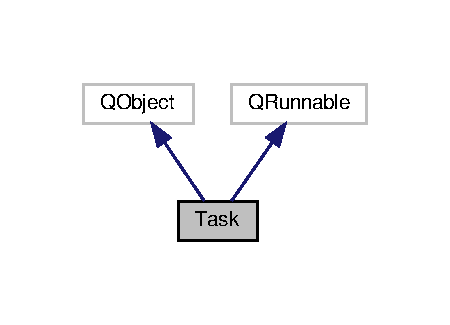
\includegraphics[width=216pt]{classTask__inherit__graph}
\end{center}
\end{figure}


Граф связей класса Task\+:\nopagebreak
\begin{figure}[H]
\begin{center}
\leavevmode
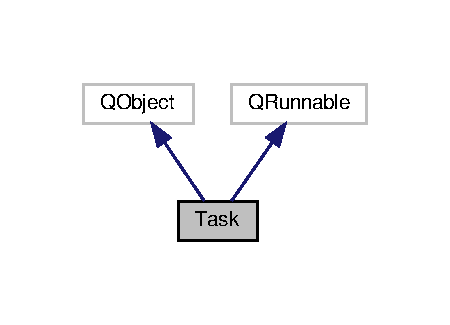
\includegraphics[width=216pt]{classTask__coll__graph}
\end{center}
\end{figure}
\subsection*{Сигналы}
\begin{DoxyCompactItemize}
\item 
void \hyperlink{classTask_a9a38657c8c17d817273b70166f35f8e2}{Result} (Q\+Byte\+Array ba)
\begin{DoxyCompactList}\small\item\em Result. \end{DoxyCompactList}\end{DoxyCompactItemize}
\subsection*{Открытые члены}
\begin{DoxyCompactItemize}
\item 
\hyperlink{classTask_a14c504e1e0ecef1a22429d6bf80771ac}{Task} (Q\+Object $\ast$parent=nullptr)
\begin{DoxyCompactList}\small\item\em \hyperlink{classTask}{Task}. \end{DoxyCompactList}\item 
void \hyperlink{classTask_a332a2afecfed5236f3e4246a788943a1}{set\+Client\+Info} (const Q\+Byte\+Array \&ba)
\begin{DoxyCompactList}\small\item\em set\+Client\+Info \end{DoxyCompactList}\end{DoxyCompactItemize}
\subsection*{Защищенные члены}
\begin{DoxyCompactItemize}
\item 
void \hyperlink{classTask_a034b41e0d81a3dc01804bbc3f73a25f2}{run} ()
\begin{DoxyCompactList}\small\item\em run \end{DoxyCompactList}\end{DoxyCompactItemize}
\subsection*{Закрытые данные}
\begin{DoxyCompactItemize}
\item 
Q\+Byte\+Array \hyperlink{classTask_ac961587d9c0cc627b69ead09f2311834}{m\+\_\+client\+\_\+request}
\begin{DoxyCompactList}\small\item\em m\+\_\+client\+\_\+request \end{DoxyCompactList}\end{DoxyCompactItemize}


\subsection{Подробное описание}
Класс задачи 

\begin{DoxyAuthor}{Автор}
Илья Трефилов 
\end{DoxyAuthor}
\begin{DoxyDate}{Дата}
01.\+12.\+2018
\end{DoxyDate}
Класс задачи выполняемой в отдельном потоке 

\subsection{Конструктор(ы)}
\mbox{\Hypertarget{classTask_a14c504e1e0ecef1a22429d6bf80771ac}\label{classTask_a14c504e1e0ecef1a22429d6bf80771ac}} 
\index{Task@{Task}!Task@{Task}}
\index{Task@{Task}!Task@{Task}}
\subsubsection{\texorpdfstring{Task()}{Task()}}
{\footnotesize\ttfamily Task\+::\+Task (\begin{DoxyParamCaption}\item[{Q\+Object $\ast$}]{parent = {\ttfamily nullptr} }\end{DoxyParamCaption})}



\hyperlink{classTask}{Task}. 


\begin{DoxyParams}{Аргументы}
{\em parent} & Указатель на родительский объект\\
\hline
\end{DoxyParams}
Конструктор класса задачи 

\subsection{Методы}
\mbox{\Hypertarget{classTask_a9a38657c8c17d817273b70166f35f8e2}\label{classTask_a9a38657c8c17d817273b70166f35f8e2}} 
\index{Task@{Task}!Result@{Result}}
\index{Result@{Result}!Task@{Task}}
\subsubsection{\texorpdfstring{Result}{Result}}
{\footnotesize\ttfamily void Task\+::\+Result (\begin{DoxyParamCaption}\item[{Q\+Byte\+Array}]{ba }\end{DoxyParamCaption})\hspace{0.3cm}{\ttfamily [signal]}}



Result. 


\begin{DoxyParams}{Аргументы}
{\em ba} & Набор байт\\
\hline
\end{DoxyParams}
Функция для отправки сигнала из отдельного потока в вызывающий объект типа \hyperlink{classClient}{Client} \mbox{\Hypertarget{classTask_a034b41e0d81a3dc01804bbc3f73a25f2}\label{classTask_a034b41e0d81a3dc01804bbc3f73a25f2}} 
\index{Task@{Task}!run@{run}}
\index{run@{run}!Task@{Task}}
\subsubsection{\texorpdfstring{run()}{run()}}
{\footnotesize\ttfamily void Task\+::run (\begin{DoxyParamCaption}{ }\end{DoxyParamCaption})\hspace{0.3cm}{\ttfamily [protected]}}



run 

Функция для запуска отдельного потока при обработке информации полученной при сетевом взаимодействии \mbox{\Hypertarget{classTask_a332a2afecfed5236f3e4246a788943a1}\label{classTask_a332a2afecfed5236f3e4246a788943a1}} 
\index{Task@{Task}!set\+Client\+Info@{set\+Client\+Info}}
\index{set\+Client\+Info@{set\+Client\+Info}!Task@{Task}}
\subsubsection{\texorpdfstring{set\+Client\+Info()}{setClientInfo()}}
{\footnotesize\ttfamily void Task\+::set\+Client\+Info (\begin{DoxyParamCaption}\item[{const Q\+Byte\+Array \&}]{ba }\end{DoxyParamCaption})}



set\+Client\+Info 


\begin{DoxyParams}{Аргументы}
{\em ba} & Набор байт\\
\hline
\end{DoxyParams}
Функция для сохранения полученного набора данных из сетевого взаимодействия в память 

\subsection{Данные класса}
\mbox{\Hypertarget{classTask_ac961587d9c0cc627b69ead09f2311834}\label{classTask_ac961587d9c0cc627b69ead09f2311834}} 
\index{Task@{Task}!m\+\_\+client\+\_\+request@{m\+\_\+client\+\_\+request}}
\index{m\+\_\+client\+\_\+request@{m\+\_\+client\+\_\+request}!Task@{Task}}
\subsubsection{\texorpdfstring{m\+\_\+client\+\_\+request}{m\_client\_request}}
{\footnotesize\ttfamily Q\+Byte\+Array Task\+::m\+\_\+client\+\_\+request\hspace{0.3cm}{\ttfamily [private]}}



m\+\_\+client\+\_\+request 

Набор байт в запросе, сохраненный в память 

Объявления и описания членов классов находятся в файлах\+:\begin{DoxyCompactItemize}
\item 
\hyperlink{task_8h}{task.\+h}\item 
\hyperlink{task_8cpp}{task.\+cpp}\end{DoxyCompactItemize}

\hypertarget{classTeleMedObject}{}\section{Класс Tele\+Med\+Object}
\label{classTeleMedObject}\index{Tele\+Med\+Object@{Tele\+Med\+Object}}


Класс объекта информации в телемедицинском сеансе  




{\ttfamily \#include $<$telemedobject.\+h$>$}

\subsection*{Открытые члены}
\begin{DoxyCompactItemize}
\item 
\hyperlink{classTeleMedObject_a754462ce944702c386aa3b6191e4db33}{Tele\+Med\+Object} ()
\begin{DoxyCompactList}\small\item\em \hyperlink{classTeleMedObject}{Tele\+Med\+Object}. \end{DoxyCompactList}\item 
\hyperlink{classTeleMedObject_a38ee0e32441775b2f4f10907b672af44}{Tele\+Med\+Object} (Q\+Image img, \hyperlink{tagshelpers_8h_ae25d30658f61420b88a380dc9e40bb74}{dicom\+Dict} dict, \hyperlink{dbform_8h_a1ec1a645f41e1c6544d384ca863a936c}{add\+Info\+Map} map)
\begin{DoxyCompactList}\small\item\em \hyperlink{classTeleMedObject}{Tele\+Med\+Object}. \end{DoxyCompactList}\item 
\hyperlink{classTeleMedObject_ac0e5013f81a28e85101305fd8b7f6a59}{Tele\+Med\+Object} (const Q\+Json\+Document \&doc)
\begin{DoxyCompactList}\small\item\em \hyperlink{classTeleMedObject}{Tele\+Med\+Object}. \end{DoxyCompactList}\item 
Q\+String \hyperlink{classTeleMedObject_a5d79f3bf01cc9ee2b714f9fa1da422df}{get\+Responser} () const
\begin{DoxyCompactList}\small\item\em get\+Responser \end{DoxyCompactList}\item 
Q\+Json\+Document \hyperlink{classTeleMedObject_a37d8e7cede94ef1695171d35c6c0c1ce}{to\+Json} ()
\begin{DoxyCompactList}\small\item\em to\+Json \end{DoxyCompactList}\item 
Q\+Image \hyperlink{classTeleMedObject_a69c34b50bb901268d193bbbb7a7698c5}{get\+Image} () const
\begin{DoxyCompactList}\small\item\em get\+Image \end{DoxyCompactList}\item 
\hyperlink{tagshelpers_8h_ae25d30658f61420b88a380dc9e40bb74}{dicom\+Dict} \hyperlink{classTeleMedObject_a66119d8882d0e8319d337a559bfa78a3}{get\+Dicom\+Dict} () const
\begin{DoxyCompactList}\small\item\em get\+Dicom\+Dict \end{DoxyCompactList}\item 
\hyperlink{dbform_8h_a1ec1a645f41e1c6544d384ca863a936c}{add\+Info\+Map} \hyperlink{classTeleMedObject_a56def4aa26d190a557014d9a3d99099f}{get\+Info\+Map} () const
\begin{DoxyCompactList}\small\item\em get\+Info\+Map \end{DoxyCompactList}\item 
bool \hyperlink{classTeleMedObject_a651ae9fa2690217a8327d194682ef60c}{is\+Empty} ()
\begin{DoxyCompactList}\small\item\em is\+Empty \end{DoxyCompactList}\item 
\hyperlink{classTeleMedObject_a6d60cc13e1b1812938cb9a7277c49d43}{$\sim$\+Tele\+Med\+Object} ()
\end{DoxyCompactItemize}
\subsection*{Закрытые данные}
\begin{DoxyCompactItemize}
\item 
Q\+Image \hyperlink{classTeleMedObject_a4ea4fc9f1c9e7f7e7760b1c7db163789}{m\+\_\+img}
\begin{DoxyCompactList}\small\item\em m\+\_\+img \end{DoxyCompactList}\item 
\hyperlink{tagshelpers_8h_ae25d30658f61420b88a380dc9e40bb74}{dicom\+Dict} \hyperlink{classTeleMedObject_a15a8c04c55623d826a04908a949fce31}{m\+\_\+dicom\+Dict}
\begin{DoxyCompactList}\small\item\em m\+\_\+dicom\+Dict \end{DoxyCompactList}\item 
\hyperlink{dbform_8h_a1ec1a645f41e1c6544d384ca863a936c}{add\+Info\+Map} \hyperlink{classTeleMedObject_a812a8fdb794711a94a9fc0fa4f1de27e}{m\+\_\+add\+Info\+Map}
\begin{DoxyCompactList}\small\item\em m\+\_\+add\+Info\+Map \end{DoxyCompactList}\end{DoxyCompactItemize}


\subsection{Подробное описание}
Класс объекта информации в телемедицинском сеансе 

\begin{DoxyAuthor}{Автор}
Илья Трефилов 
\end{DoxyAuthor}
\begin{DoxyDate}{Дата}
01.\+12.\+2018
\end{DoxyDate}
Данный класс предназначен для построения объекта информации для передачи\textbackslash{}получения в телемедицинском сеансе 

\subsection{Конструктор(ы)}
\mbox{\Hypertarget{classTeleMedObject_a754462ce944702c386aa3b6191e4db33}\label{classTeleMedObject_a754462ce944702c386aa3b6191e4db33}} 
\index{Tele\+Med\+Object@{Tele\+Med\+Object}!Tele\+Med\+Object@{Tele\+Med\+Object}}
\index{Tele\+Med\+Object@{Tele\+Med\+Object}!Tele\+Med\+Object@{Tele\+Med\+Object}}
\subsubsection{\texorpdfstring{Tele\+Med\+Object()}{TeleMedObject()}\hspace{0.1cm}{\footnotesize\ttfamily [1/3]}}
{\footnotesize\ttfamily Tele\+Med\+Object\+::\+Tele\+Med\+Object (\begin{DoxyParamCaption}{ }\end{DoxyParamCaption})\hspace{0.3cm}{\ttfamily [inline]}}



\hyperlink{classTeleMedObject}{Tele\+Med\+Object}. 

Конструктор по умолчанию \mbox{\Hypertarget{classTeleMedObject_a38ee0e32441775b2f4f10907b672af44}\label{classTeleMedObject_a38ee0e32441775b2f4f10907b672af44}} 
\index{Tele\+Med\+Object@{Tele\+Med\+Object}!Tele\+Med\+Object@{Tele\+Med\+Object}}
\index{Tele\+Med\+Object@{Tele\+Med\+Object}!Tele\+Med\+Object@{Tele\+Med\+Object}}
\subsubsection{\texorpdfstring{Tele\+Med\+Object()}{TeleMedObject()}\hspace{0.1cm}{\footnotesize\ttfamily [2/3]}}
{\footnotesize\ttfamily Tele\+Med\+Object\+::\+Tele\+Med\+Object (\begin{DoxyParamCaption}\item[{Q\+Image}]{img,  }\item[{\hyperlink{tagshelpers_8h_ae25d30658f61420b88a380dc9e40bb74}{dicom\+Dict}}]{dict,  }\item[{\hyperlink{dbform_8h_a1ec1a645f41e1c6544d384ca863a936c}{add\+Info\+Map}}]{map }\end{DoxyParamCaption})}



\hyperlink{classTeleMedObject}{Tele\+Med\+Object}. 


\begin{DoxyParams}{Аргументы}
{\em img} & Изображение \\
\hline
{\em dict} & Словарь с данными из исследования \\
\hline
{\em map} & Словарь с дополнительными данными о запросе\textbackslash{}ответе\\
\hline
\end{DoxyParams}
Конструктор выбрасывает исключение при невалидных входных данных (пустые данные) \mbox{\Hypertarget{classTeleMedObject_ac0e5013f81a28e85101305fd8b7f6a59}\label{classTeleMedObject_ac0e5013f81a28e85101305fd8b7f6a59}} 
\index{Tele\+Med\+Object@{Tele\+Med\+Object}!Tele\+Med\+Object@{Tele\+Med\+Object}}
\index{Tele\+Med\+Object@{Tele\+Med\+Object}!Tele\+Med\+Object@{Tele\+Med\+Object}}
\subsubsection{\texorpdfstring{Tele\+Med\+Object()}{TeleMedObject()}\hspace{0.1cm}{\footnotesize\ttfamily [3/3]}}
{\footnotesize\ttfamily Tele\+Med\+Object\+::\+Tele\+Med\+Object (\begin{DoxyParamCaption}\item[{const Q\+Json\+Document \&}]{doc }\end{DoxyParamCaption})}



\hyperlink{classTeleMedObject}{Tele\+Med\+Object}. 


\begin{DoxyParams}{Аргументы}
{\em doc} & Информация в виде json\\
\hline
\end{DoxyParams}
Конструктор для построения объекта из типа json В данном виде данные передаются по сети \mbox{\Hypertarget{classTeleMedObject_a6d60cc13e1b1812938cb9a7277c49d43}\label{classTeleMedObject_a6d60cc13e1b1812938cb9a7277c49d43}} 
\index{Tele\+Med\+Object@{Tele\+Med\+Object}!````~Tele\+Med\+Object@{$\sim$\+Tele\+Med\+Object}}
\index{````~Tele\+Med\+Object@{$\sim$\+Tele\+Med\+Object}!Tele\+Med\+Object@{Tele\+Med\+Object}}
\subsubsection{\texorpdfstring{$\sim$\+Tele\+Med\+Object()}{~TeleMedObject()}}
{\footnotesize\ttfamily Tele\+Med\+Object\+::$\sim$\+Tele\+Med\+Object (\begin{DoxyParamCaption}{ }\end{DoxyParamCaption})\hspace{0.3cm}{\ttfamily [inline]}}



\subsection{Методы}
\mbox{\Hypertarget{classTeleMedObject_a66119d8882d0e8319d337a559bfa78a3}\label{classTeleMedObject_a66119d8882d0e8319d337a559bfa78a3}} 
\index{Tele\+Med\+Object@{Tele\+Med\+Object}!get\+Dicom\+Dict@{get\+Dicom\+Dict}}
\index{get\+Dicom\+Dict@{get\+Dicom\+Dict}!Tele\+Med\+Object@{Tele\+Med\+Object}}
\subsubsection{\texorpdfstring{get\+Dicom\+Dict()}{getDicomDict()}}
{\footnotesize\ttfamily \hyperlink{tagshelpers_8h_ae25d30658f61420b88a380dc9e40bb74}{dicom\+Dict} Tele\+Med\+Object\+::get\+Dicom\+Dict (\begin{DoxyParamCaption}{ }\end{DoxyParamCaption}) const}



get\+Dicom\+Dict 

\begin{DoxyReturn}{Возвращает}
Словарь с информацией об исследовании
\end{DoxyReturn}
Функция возвращает словарь с информацией об исследовании \mbox{\Hypertarget{classTeleMedObject_a69c34b50bb901268d193bbbb7a7698c5}\label{classTeleMedObject_a69c34b50bb901268d193bbbb7a7698c5}} 
\index{Tele\+Med\+Object@{Tele\+Med\+Object}!get\+Image@{get\+Image}}
\index{get\+Image@{get\+Image}!Tele\+Med\+Object@{Tele\+Med\+Object}}
\subsubsection{\texorpdfstring{get\+Image()}{getImage()}}
{\footnotesize\ttfamily Q\+Image Tele\+Med\+Object\+::get\+Image (\begin{DoxyParamCaption}{ }\end{DoxyParamCaption}) const}



get\+Image 

\begin{DoxyReturn}{Возвращает}
Изображение
\end{DoxyReturn}
Получение изображения из объекта \mbox{\Hypertarget{classTeleMedObject_a56def4aa26d190a557014d9a3d99099f}\label{classTeleMedObject_a56def4aa26d190a557014d9a3d99099f}} 
\index{Tele\+Med\+Object@{Tele\+Med\+Object}!get\+Info\+Map@{get\+Info\+Map}}
\index{get\+Info\+Map@{get\+Info\+Map}!Tele\+Med\+Object@{Tele\+Med\+Object}}
\subsubsection{\texorpdfstring{get\+Info\+Map()}{getInfoMap()}}
{\footnotesize\ttfamily \hyperlink{dbform_8h_a1ec1a645f41e1c6544d384ca863a936c}{add\+Info\+Map} Tele\+Med\+Object\+::get\+Info\+Map (\begin{DoxyParamCaption}{ }\end{DoxyParamCaption}) const}



get\+Info\+Map 

\begin{DoxyReturn}{Возвращает}
Словарь с информацией о запросе\textbackslash{}ответе
\end{DoxyReturn}
Функция возвращает словарь с информацией о запросе\textbackslash{}ответе \mbox{\Hypertarget{classTeleMedObject_a5d79f3bf01cc9ee2b714f9fa1da422df}\label{classTeleMedObject_a5d79f3bf01cc9ee2b714f9fa1da422df}} 
\index{Tele\+Med\+Object@{Tele\+Med\+Object}!get\+Responser@{get\+Responser}}
\index{get\+Responser@{get\+Responser}!Tele\+Med\+Object@{Tele\+Med\+Object}}
\subsubsection{\texorpdfstring{get\+Responser()}{getResponser()}}
{\footnotesize\ttfamily Q\+String Tele\+Med\+Object\+::get\+Responser (\begin{DoxyParamCaption}{ }\end{DoxyParamCaption}) const}



get\+Responser 

\begin{DoxyReturn}{Возвращает}
Строка идентифицирующая отвечающую сторону 
\end{DoxyReturn}
\mbox{\Hypertarget{classTeleMedObject_a651ae9fa2690217a8327d194682ef60c}\label{classTeleMedObject_a651ae9fa2690217a8327d194682ef60c}} 
\index{Tele\+Med\+Object@{Tele\+Med\+Object}!is\+Empty@{is\+Empty}}
\index{is\+Empty@{is\+Empty}!Tele\+Med\+Object@{Tele\+Med\+Object}}
\subsubsection{\texorpdfstring{is\+Empty()}{isEmpty()}}
{\footnotesize\ttfamily bool Tele\+Med\+Object\+::is\+Empty (\begin{DoxyParamCaption}{ }\end{DoxyParamCaption})}



is\+Empty 

\begin{DoxyReturn}{Возвращает}
true -\/ если объект информации пустой
\end{DoxyReturn}
Функция проверяет, что объект информации пустой \mbox{\Hypertarget{classTeleMedObject_a37d8e7cede94ef1695171d35c6c0c1ce}\label{classTeleMedObject_a37d8e7cede94ef1695171d35c6c0c1ce}} 
\index{Tele\+Med\+Object@{Tele\+Med\+Object}!to\+Json@{to\+Json}}
\index{to\+Json@{to\+Json}!Tele\+Med\+Object@{Tele\+Med\+Object}}
\subsubsection{\texorpdfstring{to\+Json()}{toJson()}}
{\footnotesize\ttfamily Q\+Json\+Document Tele\+Med\+Object\+::to\+Json (\begin{DoxyParamCaption}{ }\end{DoxyParamCaption})}



to\+Json 

\begin{DoxyReturn}{Возвращает}
Информация об объекте в виде json
\end{DoxyReturn}
Функция строит объект информации в виде документа json 

\subsection{Данные класса}
\mbox{\Hypertarget{classTeleMedObject_a812a8fdb794711a94a9fc0fa4f1de27e}\label{classTeleMedObject_a812a8fdb794711a94a9fc0fa4f1de27e}} 
\index{Tele\+Med\+Object@{Tele\+Med\+Object}!m\+\_\+add\+Info\+Map@{m\+\_\+add\+Info\+Map}}
\index{m\+\_\+add\+Info\+Map@{m\+\_\+add\+Info\+Map}!Tele\+Med\+Object@{Tele\+Med\+Object}}
\subsubsection{\texorpdfstring{m\+\_\+add\+Info\+Map}{m\_addInfoMap}}
{\footnotesize\ttfamily \hyperlink{dbform_8h_a1ec1a645f41e1c6544d384ca863a936c}{add\+Info\+Map} Tele\+Med\+Object\+::m\+\_\+add\+Info\+Map\hspace{0.3cm}{\ttfamily [private]}}



m\+\_\+add\+Info\+Map 

Словарь с информацией о запросе\textbackslash{}ответе \mbox{\Hypertarget{classTeleMedObject_a15a8c04c55623d826a04908a949fce31}\label{classTeleMedObject_a15a8c04c55623d826a04908a949fce31}} 
\index{Tele\+Med\+Object@{Tele\+Med\+Object}!m\+\_\+dicom\+Dict@{m\+\_\+dicom\+Dict}}
\index{m\+\_\+dicom\+Dict@{m\+\_\+dicom\+Dict}!Tele\+Med\+Object@{Tele\+Med\+Object}}
\subsubsection{\texorpdfstring{m\+\_\+dicom\+Dict}{m\_dicomDict}}
{\footnotesize\ttfamily \hyperlink{tagshelpers_8h_ae25d30658f61420b88a380dc9e40bb74}{dicom\+Dict} Tele\+Med\+Object\+::m\+\_\+dicom\+Dict\hspace{0.3cm}{\ttfamily [private]}}



m\+\_\+dicom\+Dict 

Словарь с информацией об исследовании \mbox{\Hypertarget{classTeleMedObject_a4ea4fc9f1c9e7f7e7760b1c7db163789}\label{classTeleMedObject_a4ea4fc9f1c9e7f7e7760b1c7db163789}} 
\index{Tele\+Med\+Object@{Tele\+Med\+Object}!m\+\_\+img@{m\+\_\+img}}
\index{m\+\_\+img@{m\+\_\+img}!Tele\+Med\+Object@{Tele\+Med\+Object}}
\subsubsection{\texorpdfstring{m\+\_\+img}{m\_img}}
{\footnotesize\ttfamily Q\+Image Tele\+Med\+Object\+::m\+\_\+img\hspace{0.3cm}{\ttfamily [private]}}



m\+\_\+img 

Изображение исследования 

Объявления и описания членов классов находятся в файлах\+:\begin{DoxyCompactItemize}
\item 
\hyperlink{telemedobject_8h}{telemedobject.\+h}\item 
\hyperlink{telemedobject_8cpp}{telemedobject.\+cpp}\end{DoxyCompactItemize}

\hypertarget{classTeleMedObjException}{}\section{Класс Tele\+Med\+Obj\+Exception}
\label{classTeleMedObjException}\index{Tele\+Med\+Obj\+Exception@{Tele\+Med\+Obj\+Exception}}


Класс исключения при построении объекта информации  




{\ttfamily \#include $<$telemedobject.\+h$>$}



Граф наследования\+:Tele\+Med\+Obj\+Exception\+:\nopagebreak
\begin{figure}[H]
\begin{center}
\leavevmode
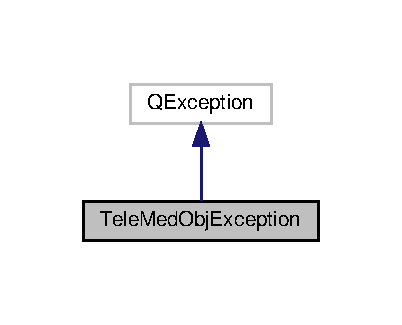
\includegraphics[width=193pt]{classTeleMedObjException__inherit__graph}
\end{center}
\end{figure}


Граф связей класса Tele\+Med\+Obj\+Exception\+:\nopagebreak
\begin{figure}[H]
\begin{center}
\leavevmode
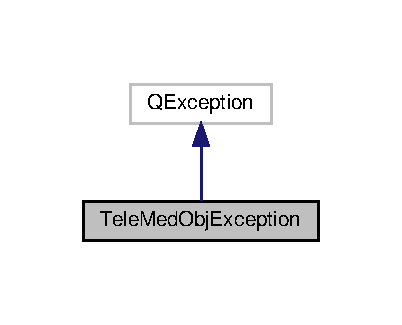
\includegraphics[width=193pt]{classTeleMedObjException__coll__graph}
\end{center}
\end{figure}
\subsection*{Открытые члены}
\begin{DoxyCompactItemize}
\item 
\hyperlink{classTeleMedObjException_a351ba22504a9acf7ed560fd6659013da}{Tele\+Med\+Obj\+Exception} (const char $\ast$error\+String)
\begin{DoxyCompactList}\small\item\em \hyperlink{classTeleMedObjException}{Tele\+Med\+Obj\+Exception}. \end{DoxyCompactList}\item 
virtual void \hyperlink{classTeleMedObjException_a367ddc1ca442487da31f7557bd4bc6ff}{raise} () const
\begin{DoxyCompactList}\small\item\em raise \end{DoxyCompactList}\item 
virtual \hyperlink{classTeleMedObjException}{Tele\+Med\+Obj\+Exception} $\ast$ \hyperlink{classTeleMedObjException_a32f7656b034f2a49c7622def17ff8b63}{clone} () const
\begin{DoxyCompactList}\small\item\em clone \end{DoxyCompactList}\item 
virtual const char $\ast$ \hyperlink{classTeleMedObjException_a4d0745f8597c3273301fa88000e35cd8}{what} () const noexcept
\begin{DoxyCompactList}\small\item\em what \end{DoxyCompactList}\end{DoxyCompactItemize}
\subsection*{Закрытые данные}
\begin{DoxyCompactItemize}
\item 
const char $\ast$ \hyperlink{classTeleMedObjException_a91ff803c7abad201ad2bb96a2149ea5e}{m\+\_\+error\+String}
\begin{DoxyCompactList}\small\item\em m\+\_\+error\+String \end{DoxyCompactList}\end{DoxyCompactItemize}


\subsection{Подробное описание}
Класс исключения при построении объекта информации 

\begin{DoxyAuthor}{Автор}
Илья Трефилов 
\end{DoxyAuthor}
\begin{DoxyDate}{Дата}
01.\+12.\+2018
\end{DoxyDate}
Данный класс предназначен для сообщения о нештатных ситуациях при обработке объекта информации 

\subsection{Конструктор(ы)}
\mbox{\Hypertarget{classTeleMedObjException_a351ba22504a9acf7ed560fd6659013da}\label{classTeleMedObjException_a351ba22504a9acf7ed560fd6659013da}} 
\index{Tele\+Med\+Obj\+Exception@{Tele\+Med\+Obj\+Exception}!Tele\+Med\+Obj\+Exception@{Tele\+Med\+Obj\+Exception}}
\index{Tele\+Med\+Obj\+Exception@{Tele\+Med\+Obj\+Exception}!Tele\+Med\+Obj\+Exception@{Tele\+Med\+Obj\+Exception}}
\subsubsection{\texorpdfstring{Tele\+Med\+Obj\+Exception()}{TeleMedObjException()}}
{\footnotesize\ttfamily Tele\+Med\+Obj\+Exception\+::\+Tele\+Med\+Obj\+Exception (\begin{DoxyParamCaption}\item[{const char $\ast$}]{error\+String }\end{DoxyParamCaption})\hspace{0.3cm}{\ttfamily [inline]}}



\hyperlink{classTeleMedObjException}{Tele\+Med\+Obj\+Exception}. 


\begin{DoxyParams}{Аргументы}
{\em error\+String} & Сообщение об ошибке\\
\hline
\end{DoxyParams}
Конструктор класса исключения 

\subsection{Методы}
\mbox{\Hypertarget{classTeleMedObjException_a32f7656b034f2a49c7622def17ff8b63}\label{classTeleMedObjException_a32f7656b034f2a49c7622def17ff8b63}} 
\index{Tele\+Med\+Obj\+Exception@{Tele\+Med\+Obj\+Exception}!clone@{clone}}
\index{clone@{clone}!Tele\+Med\+Obj\+Exception@{Tele\+Med\+Obj\+Exception}}
\subsubsection{\texorpdfstring{clone()}{clone()}}
{\footnotesize\ttfamily virtual \hyperlink{classTeleMedObjException}{Tele\+Med\+Obj\+Exception}$\ast$ Tele\+Med\+Obj\+Exception\+::clone (\begin{DoxyParamCaption}{ }\end{DoxyParamCaption}) const\hspace{0.3cm}{\ttfamily [inline]}, {\ttfamily [virtual]}}



clone 

\begin{DoxyReturn}{Возвращает}
Объект исключения
\end{DoxyReturn}
Функция для выделения памяти под объект исключения \mbox{\Hypertarget{classTeleMedObjException_a367ddc1ca442487da31f7557bd4bc6ff}\label{classTeleMedObjException_a367ddc1ca442487da31f7557bd4bc6ff}} 
\index{Tele\+Med\+Obj\+Exception@{Tele\+Med\+Obj\+Exception}!raise@{raise}}
\index{raise@{raise}!Tele\+Med\+Obj\+Exception@{Tele\+Med\+Obj\+Exception}}
\subsubsection{\texorpdfstring{raise()}{raise()}}
{\footnotesize\ttfamily virtual void Tele\+Med\+Obj\+Exception\+::raise (\begin{DoxyParamCaption}{ }\end{DoxyParamCaption}) const\hspace{0.3cm}{\ttfamily [inline]}, {\ttfamily [virtual]}}



raise 

Функция для вызова исключения в программе \mbox{\Hypertarget{classTeleMedObjException_a4d0745f8597c3273301fa88000e35cd8}\label{classTeleMedObjException_a4d0745f8597c3273301fa88000e35cd8}} 
\index{Tele\+Med\+Obj\+Exception@{Tele\+Med\+Obj\+Exception}!what@{what}}
\index{what@{what}!Tele\+Med\+Obj\+Exception@{Tele\+Med\+Obj\+Exception}}
\subsubsection{\texorpdfstring{what()}{what()}}
{\footnotesize\ttfamily virtual const char$\ast$ Tele\+Med\+Obj\+Exception\+::what (\begin{DoxyParamCaption}{ }\end{DoxyParamCaption}) const\hspace{0.3cm}{\ttfamily [inline]}, {\ttfamily [virtual]}, {\ttfamily [noexcept]}}



what 

\begin{DoxyReturn}{Возвращает}
Сообщение об ошибке
\end{DoxyReturn}
Функция для получения сообщения об ошибке при исключении в программе 

\subsection{Данные класса}
\mbox{\Hypertarget{classTeleMedObjException_a91ff803c7abad201ad2bb96a2149ea5e}\label{classTeleMedObjException_a91ff803c7abad201ad2bb96a2149ea5e}} 
\index{Tele\+Med\+Obj\+Exception@{Tele\+Med\+Obj\+Exception}!m\+\_\+error\+String@{m\+\_\+error\+String}}
\index{m\+\_\+error\+String@{m\+\_\+error\+String}!Tele\+Med\+Obj\+Exception@{Tele\+Med\+Obj\+Exception}}
\subsubsection{\texorpdfstring{m\+\_\+error\+String}{m\_errorString}}
{\footnotesize\ttfamily const char$\ast$ Tele\+Med\+Obj\+Exception\+::m\+\_\+error\+String\hspace{0.3cm}{\ttfamily [private]}}



m\+\_\+error\+String 

Строка с сообщением об ошибке 

Объявления и описания членов класса находятся в файле\+:\begin{DoxyCompactItemize}
\item 
\hyperlink{telemedobject_8h}{telemedobject.\+h}\end{DoxyCompactItemize}

\hypertarget{classViewerForm}{}\section{Класс Viewer\+Form}
\label{classViewerForm}\index{Viewer\+Form@{Viewer\+Form}}


Класс формы для отображения файлов dcm.  




{\ttfamily \#include $<$viewerform.\+h$>$}



Граф наследования\+:Viewer\+Form\+:\nopagebreak
\begin{figure}[H]
\begin{center}
\leavevmode
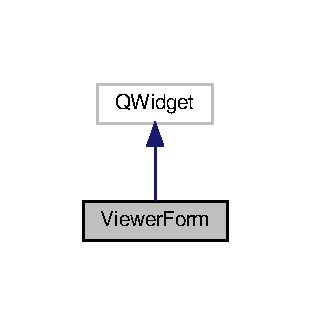
\includegraphics[width=149pt]{classViewerForm__inherit__graph}
\end{center}
\end{figure}


Граф связей класса Viewer\+Form\+:\nopagebreak
\begin{figure}[H]
\begin{center}
\leavevmode
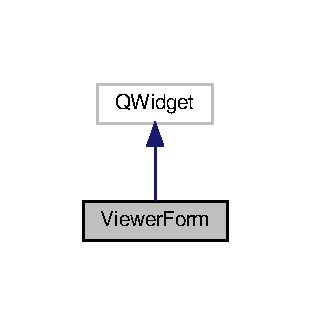
\includegraphics[width=149pt]{classViewerForm__coll__graph}
\end{center}
\end{figure}
\subsection*{Сигналы}
\begin{DoxyCompactItemize}
\item 
void \hyperlink{classViewerForm_a5d3adb46be46748d665e38e47decdf2c}{send\+Insert\+Signal} (Q\+String \&name, Q\+Image \&image, \hyperlink{tagshelpers_8h_ae25d30658f61420b88a380dc9e40bb74}{dicom\+Dict} \&dict, \hyperlink{dbform_8h_a1ec1a645f41e1c6544d384ca863a936c}{add\+Info\+Map} \&info\+Map)
\begin{DoxyCompactList}\small\item\em send\+Insert\+Signal \end{DoxyCompactList}\end{DoxyCompactItemize}
\subsection*{Открытые члены}
\begin{DoxyCompactItemize}
\item 
void \hyperlink{classViewerForm_ae36251270d9db1b29cecb787876dfdc1}{show\+Event} (Q\+Show\+Event $\ast$)
\begin{DoxyCompactList}\small\item\em show\+Event \end{DoxyCompactList}\item 
\hyperlink{classViewerForm_ac64816c194730c3d825edbb7b7773dee}{Viewer\+Form} (Q\+Widget $\ast$parent=nullptr)
\begin{DoxyCompactList}\small\item\em \hyperlink{classViewerForm}{Viewer\+Form}. \end{DoxyCompactList}\item 
\hyperlink{classViewerForm_ac75f02831e65d75ef9b9843d9a180ee4}{$\sim$\+Viewer\+Form} ()
\end{DoxyCompactItemize}
\subsection*{Открытые атрибуты}
\begin{DoxyCompactItemize}
\item 
Q\+String \hyperlink{classViewerForm_ab2f0d1908098c723c3f52e89f69e46f4}{file\+Name}
\begin{DoxyCompactList}\small\item\em file\+Name \end{DoxyCompactList}\item 
Q\+Graphics\+Scene $\ast$ \hyperlink{classViewerForm_a65bd3ad0087e45497639bb3050084d0a}{scene}
\begin{DoxyCompactList}\small\item\em scene \end{DoxyCompactList}\end{DoxyCompactItemize}
\subsection*{Закрытые типы}
\begin{DoxyCompactItemize}
\item 
enum \hyperlink{classViewerForm_adb304869a7f4e7573df0e018cd03a845}{m\+\_\+columns} \{ \hyperlink{classViewerForm_adb304869a7f4e7573df0e018cd03a845a530374d647e5499f1079a433971650fd}{Tag}, 
\hyperlink{classViewerForm_adb304869a7f4e7573df0e018cd03a845a4106ad6b7649446b55c2fc0c9e546ca2}{Description}, 
\hyperlink{classViewerForm_adb304869a7f4e7573df0e018cd03a845a36c75b35df69479c62b3a215e7c8bb64}{Value}
 \}\begin{DoxyCompactList}\small\item\em The m\+\_\+columns enum. \end{DoxyCompactList}
\end{DoxyCompactItemize}
\subsection*{Закрытые слоты}
\begin{DoxyCompactItemize}
\item 
void \hyperlink{classViewerForm_aebe4c92a2d951281558a7074347a7ec7}{on\+\_\+load\+Image\+Button\+\_\+clicked} ()
\begin{DoxyCompactList}\small\item\em on\+\_\+load\+Image\+Button\+\_\+clicked \end{DoxyCompactList}\item 
void \hyperlink{classViewerForm_a298b0181b562b7521e62212db1976cdd}{on\+\_\+dicom\+Attribute\+Table\+Widget\+\_\+cell\+Changed} (int row, int column)
\begin{DoxyCompactList}\small\item\em on\+\_\+dicom\+Attribute\+Table\+Widget\+\_\+cell\+Changed \end{DoxyCompactList}\end{DoxyCompactItemize}
\subsection*{Закрытые члены}
\begin{DoxyCompactItemize}
\item 
bool \hyperlink{classViewerForm_a8b7701ce8061967e519b691aa5a9ec93}{show\+Message\+Box\+Asking\+For\+Change} ()
\begin{DoxyCompactList}\small\item\em show\+Message\+Box\+Asking\+For\+Change \end{DoxyCompactList}\item 
void \hyperlink{classViewerForm_a2c109da65b355c5e9712a148b01ee7f3}{init\+Table} (const \hyperlink{tagshelpers_8h_ae25d30658f61420b88a380dc9e40bb74}{dicom\+Dict} \&dict)
\begin{DoxyCompactList}\small\item\em init\+Table \end{DoxyCompactList}\end{DoxyCompactItemize}
\subsection*{Закрытые данные}
\begin{DoxyCompactItemize}
\item 
bool \hyperlink{classViewerForm_a38c70bda1c65ed5a26e06eb73233ffb2}{m\+\_\+change\+Allowed}
\begin{DoxyCompactList}\small\item\em m\+\_\+change\+Allowed \end{DoxyCompactList}\item 
const int \hyperlink{classViewerForm_aec8417758835f4b71657413c06eec160}{m\+\_\+table\+\_\+columns\+\_\+count} = 3
\begin{DoxyCompactList}\small\item\em m\+\_\+table\+\_\+columns\+\_\+count \end{DoxyCompactList}\item 
Ui\+::\+Viewer\+Form $\ast$ \hyperlink{classViewerForm_a0e264f78c6535b2442b03629ebdc0347}{ui}
\begin{DoxyCompactList}\small\item\em ui Указатель на объект интерфейса для данного класса \end{DoxyCompactList}\end{DoxyCompactItemize}


\subsection{Подробное описание}
Класс формы для отображения файлов dcm. 

\begin{DoxyAuthor}{Автор}
Илья Трефилов 
\end{DoxyAuthor}
\begin{DoxyDate}{Дата}
01.\+12.\+2018 
\end{DoxyDate}


\subsection{Перечисления}
\mbox{\Hypertarget{classViewerForm_adb304869a7f4e7573df0e018cd03a845}\label{classViewerForm_adb304869a7f4e7573df0e018cd03a845}} 
\index{Viewer\+Form@{Viewer\+Form}!m\+\_\+columns@{m\+\_\+columns}}
\index{m\+\_\+columns@{m\+\_\+columns}!Viewer\+Form@{Viewer\+Form}}
\subsubsection{\texorpdfstring{m\+\_\+columns}{m\_columns}}
{\footnotesize\ttfamily enum \hyperlink{classViewerForm_adb304869a7f4e7573df0e018cd03a845}{Viewer\+Form\+::m\+\_\+columns}\hspace{0.3cm}{\ttfamily [private]}}



The m\+\_\+columns enum. 

Отображение колонок таблицы на колонки в базе данных \begin{DoxyEnumFields}{Элементы перечислений}
\raisebox{\heightof{T}}[0pt][0pt]{\index{Tag@{Tag}!Viewer\+Form@{Viewer\+Form}}\index{Viewer\+Form@{Viewer\+Form}!Tag@{Tag}}}\mbox{\Hypertarget{classViewerForm_adb304869a7f4e7573df0e018cd03a845a530374d647e5499f1079a433971650fd}\label{classViewerForm_adb304869a7f4e7573df0e018cd03a845a530374d647e5499f1079a433971650fd}} 
Tag&\\
\hline

\raisebox{\heightof{T}}[0pt][0pt]{\index{Description@{Description}!Viewer\+Form@{Viewer\+Form}}\index{Viewer\+Form@{Viewer\+Form}!Description@{Description}}}\mbox{\Hypertarget{classViewerForm_adb304869a7f4e7573df0e018cd03a845a4106ad6b7649446b55c2fc0c9e546ca2}\label{classViewerForm_adb304869a7f4e7573df0e018cd03a845a4106ad6b7649446b55c2fc0c9e546ca2}} 
Description&\\
\hline

\raisebox{\heightof{T}}[0pt][0pt]{\index{Value@{Value}!Viewer\+Form@{Viewer\+Form}}\index{Viewer\+Form@{Viewer\+Form}!Value@{Value}}}\mbox{\Hypertarget{classViewerForm_adb304869a7f4e7573df0e018cd03a845a36c75b35df69479c62b3a215e7c8bb64}\label{classViewerForm_adb304869a7f4e7573df0e018cd03a845a36c75b35df69479c62b3a215e7c8bb64}} 
Value&\\
\hline

\end{DoxyEnumFields}


\subsection{Конструктор(ы)}
\mbox{\Hypertarget{classViewerForm_ac64816c194730c3d825edbb7b7773dee}\label{classViewerForm_ac64816c194730c3d825edbb7b7773dee}} 
\index{Viewer\+Form@{Viewer\+Form}!Viewer\+Form@{Viewer\+Form}}
\index{Viewer\+Form@{Viewer\+Form}!Viewer\+Form@{Viewer\+Form}}
\subsubsection{\texorpdfstring{Viewer\+Form()}{ViewerForm()}}
{\footnotesize\ttfamily Viewer\+Form\+::\+Viewer\+Form (\begin{DoxyParamCaption}\item[{Q\+Widget $\ast$}]{parent = {\ttfamily nullptr} }\end{DoxyParamCaption})\hspace{0.3cm}{\ttfamily [explicit]}}



\hyperlink{classViewerForm}{Viewer\+Form}. 


\begin{DoxyParams}{Аргументы}
{\em parent} & Указатель на родительский виджет\\
\hline
\end{DoxyParams}
Конструктор класса формы \mbox{\Hypertarget{classViewerForm_ac75f02831e65d75ef9b9843d9a180ee4}\label{classViewerForm_ac75f02831e65d75ef9b9843d9a180ee4}} 
\index{Viewer\+Form@{Viewer\+Form}!````~Viewer\+Form@{$\sim$\+Viewer\+Form}}
\index{````~Viewer\+Form@{$\sim$\+Viewer\+Form}!Viewer\+Form@{Viewer\+Form}}
\subsubsection{\texorpdfstring{$\sim$\+Viewer\+Form()}{~ViewerForm()}}
{\footnotesize\ttfamily Viewer\+Form\+::$\sim$\+Viewer\+Form (\begin{DoxyParamCaption}{ }\end{DoxyParamCaption})}



\subsection{Методы}
\mbox{\Hypertarget{classViewerForm_a2c109da65b355c5e9712a148b01ee7f3}\label{classViewerForm_a2c109da65b355c5e9712a148b01ee7f3}} 
\index{Viewer\+Form@{Viewer\+Form}!init\+Table@{init\+Table}}
\index{init\+Table@{init\+Table}!Viewer\+Form@{Viewer\+Form}}
\subsubsection{\texorpdfstring{init\+Table()}{initTable()}}
{\footnotesize\ttfamily void Viewer\+Form\+::init\+Table (\begin{DoxyParamCaption}\item[{const \hyperlink{tagshelpers_8h_ae25d30658f61420b88a380dc9e40bb74}{dicom\+Dict} \&}]{dict }\end{DoxyParamCaption})\hspace{0.3cm}{\ttfamily [private]}}



init\+Table 


\begin{DoxyParams}{Аргументы}
{\em dict} & Словарь с данными об исследовании\\
\hline
\end{DoxyParams}
Функция для инициализации таблицы данными из dcm файла \mbox{\Hypertarget{classViewerForm_a298b0181b562b7521e62212db1976cdd}\label{classViewerForm_a298b0181b562b7521e62212db1976cdd}} 
\index{Viewer\+Form@{Viewer\+Form}!on\+\_\+dicom\+Attribute\+Table\+Widget\+\_\+cell\+Changed@{on\+\_\+dicom\+Attribute\+Table\+Widget\+\_\+cell\+Changed}}
\index{on\+\_\+dicom\+Attribute\+Table\+Widget\+\_\+cell\+Changed@{on\+\_\+dicom\+Attribute\+Table\+Widget\+\_\+cell\+Changed}!Viewer\+Form@{Viewer\+Form}}
\subsubsection{\texorpdfstring{on\+\_\+dicom\+Attribute\+Table\+Widget\+\_\+cell\+Changed}{on\_dicomAttributeTableWidget\_cellChanged}}
{\footnotesize\ttfamily void Viewer\+Form\+::on\+\_\+dicom\+Attribute\+Table\+Widget\+\_\+cell\+Changed (\begin{DoxyParamCaption}\item[{int}]{row,  }\item[{int}]{column }\end{DoxyParamCaption})\hspace{0.3cm}{\ttfamily [private]}, {\ttfamily [slot]}}



on\+\_\+dicom\+Attribute\+Table\+Widget\+\_\+cell\+Changed 


\begin{DoxyParams}{Аргументы}
{\em row} & Строка \\
\hline
{\em column} & Столбец\\
\hline
\end{DoxyParams}
Слот для предложения пользователю изменить значение тега в файле Действует при изменении пользователем тега в таблице \mbox{\Hypertarget{classViewerForm_aebe4c92a2d951281558a7074347a7ec7}\label{classViewerForm_aebe4c92a2d951281558a7074347a7ec7}} 
\index{Viewer\+Form@{Viewer\+Form}!on\+\_\+load\+Image\+Button\+\_\+clicked@{on\+\_\+load\+Image\+Button\+\_\+clicked}}
\index{on\+\_\+load\+Image\+Button\+\_\+clicked@{on\+\_\+load\+Image\+Button\+\_\+clicked}!Viewer\+Form@{Viewer\+Form}}
\subsubsection{\texorpdfstring{on\+\_\+load\+Image\+Button\+\_\+clicked}{on\_loadImageButton\_clicked}}
{\footnotesize\ttfamily void Viewer\+Form\+::on\+\_\+load\+Image\+Button\+\_\+clicked (\begin{DoxyParamCaption}{ }\end{DoxyParamCaption})\hspace{0.3cm}{\ttfamily [private]}, {\ttfamily [slot]}}



on\+\_\+load\+Image\+Button\+\_\+clicked 

Слот для показа диалогового окна выбора файла \mbox{\Hypertarget{classViewerForm_a5d3adb46be46748d665e38e47decdf2c}\label{classViewerForm_a5d3adb46be46748d665e38e47decdf2c}} 
\index{Viewer\+Form@{Viewer\+Form}!send\+Insert\+Signal@{send\+Insert\+Signal}}
\index{send\+Insert\+Signal@{send\+Insert\+Signal}!Viewer\+Form@{Viewer\+Form}}
\subsubsection{\texorpdfstring{send\+Insert\+Signal}{sendInsertSignal}}
{\footnotesize\ttfamily void Viewer\+Form\+::send\+Insert\+Signal (\begin{DoxyParamCaption}\item[{Q\+String \&}]{name,  }\item[{Q\+Image \&}]{image,  }\item[{\hyperlink{tagshelpers_8h_ae25d30658f61420b88a380dc9e40bb74}{dicom\+Dict} \&}]{dict,  }\item[{\hyperlink{dbform_8h_a1ec1a645f41e1c6544d384ca863a936c}{add\+Info\+Map} \&}]{info\+Map }\end{DoxyParamCaption})\hspace{0.3cm}{\ttfamily [signal]}}



send\+Insert\+Signal 


\begin{DoxyParams}{Аргументы}
{\em name} & Имя пациента \\
\hline
{\em image} & Изображение \\
\hline
{\em dict} & Словарь с данными об исследовании \\
\hline
{\em info\+Map} & Словарь с данными о запросе\textbackslash{}ответе \\
\hline
\end{DoxyParams}
\mbox{\Hypertarget{classViewerForm_ae36251270d9db1b29cecb787876dfdc1}\label{classViewerForm_ae36251270d9db1b29cecb787876dfdc1}} 
\index{Viewer\+Form@{Viewer\+Form}!show\+Event@{show\+Event}}
\index{show\+Event@{show\+Event}!Viewer\+Form@{Viewer\+Form}}
\subsubsection{\texorpdfstring{show\+Event()}{showEvent()}}
{\footnotesize\ttfamily void Viewer\+Form\+::show\+Event (\begin{DoxyParamCaption}\item[{Q\+Show\+Event $\ast$}]{ }\end{DoxyParamCaption})}



show\+Event 

Событие отображения изображения в сцене, масштабирующее изображение по рамке сцены \mbox{\Hypertarget{classViewerForm_a8b7701ce8061967e519b691aa5a9ec93}\label{classViewerForm_a8b7701ce8061967e519b691aa5a9ec93}} 
\index{Viewer\+Form@{Viewer\+Form}!show\+Message\+Box\+Asking\+For\+Change@{show\+Message\+Box\+Asking\+For\+Change}}
\index{show\+Message\+Box\+Asking\+For\+Change@{show\+Message\+Box\+Asking\+For\+Change}!Viewer\+Form@{Viewer\+Form}}
\subsubsection{\texorpdfstring{show\+Message\+Box\+Asking\+For\+Change()}{showMessageBoxAskingForChange()}}
{\footnotesize\ttfamily bool Viewer\+Form\+::show\+Message\+Box\+Asking\+For\+Change (\begin{DoxyParamCaption}{ }\end{DoxyParamCaption})\hspace{0.3cm}{\ttfamily [private]}}



show\+Message\+Box\+Asking\+For\+Change 

\begin{DoxyReturn}{Возвращает}
true -\/ если ползователь нажал OK
\end{DoxyReturn}
Функция для отображения диалога о необходимости сохранения информации из dcm фaйла в базу 

\subsection{Данные класса}
\mbox{\Hypertarget{classViewerForm_ab2f0d1908098c723c3f52e89f69e46f4}\label{classViewerForm_ab2f0d1908098c723c3f52e89f69e46f4}} 
\index{Viewer\+Form@{Viewer\+Form}!file\+Name@{file\+Name}}
\index{file\+Name@{file\+Name}!Viewer\+Form@{Viewer\+Form}}
\subsubsection{\texorpdfstring{file\+Name}{fileName}}
{\footnotesize\ttfamily Q\+String Viewer\+Form\+::file\+Name}



file\+Name 

Имя файла на файловой системе \mbox{\Hypertarget{classViewerForm_a38c70bda1c65ed5a26e06eb73233ffb2}\label{classViewerForm_a38c70bda1c65ed5a26e06eb73233ffb2}} 
\index{Viewer\+Form@{Viewer\+Form}!m\+\_\+change\+Allowed@{m\+\_\+change\+Allowed}}
\index{m\+\_\+change\+Allowed@{m\+\_\+change\+Allowed}!Viewer\+Form@{Viewer\+Form}}
\subsubsection{\texorpdfstring{m\+\_\+change\+Allowed}{m\_changeAllowed}}
{\footnotesize\ttfamily bool Viewer\+Form\+::m\+\_\+change\+Allowed\hspace{0.3cm}{\ttfamily [private]}}



m\+\_\+change\+Allowed 

Флажок отображающий возможность изменения тега в файле \mbox{\Hypertarget{classViewerForm_aec8417758835f4b71657413c06eec160}\label{classViewerForm_aec8417758835f4b71657413c06eec160}} 
\index{Viewer\+Form@{Viewer\+Form}!m\+\_\+table\+\_\+columns\+\_\+count@{m\+\_\+table\+\_\+columns\+\_\+count}}
\index{m\+\_\+table\+\_\+columns\+\_\+count@{m\+\_\+table\+\_\+columns\+\_\+count}!Viewer\+Form@{Viewer\+Form}}
\subsubsection{\texorpdfstring{m\+\_\+table\+\_\+columns\+\_\+count}{m\_table\_columns\_count}}
{\footnotesize\ttfamily const int Viewer\+Form\+::m\+\_\+table\+\_\+columns\+\_\+count = 3\hspace{0.3cm}{\ttfamily [private]}}



m\+\_\+table\+\_\+columns\+\_\+count 

Количество столбцов в таблице виджета \mbox{\Hypertarget{classViewerForm_a65bd3ad0087e45497639bb3050084d0a}\label{classViewerForm_a65bd3ad0087e45497639bb3050084d0a}} 
\index{Viewer\+Form@{Viewer\+Form}!scene@{scene}}
\index{scene@{scene}!Viewer\+Form@{Viewer\+Form}}
\subsubsection{\texorpdfstring{scene}{scene}}
{\footnotesize\ttfamily Q\+Graphics\+Scene$\ast$ Viewer\+Form\+::scene}



scene 

Сцена для показа изображения \mbox{\Hypertarget{classViewerForm_a0e264f78c6535b2442b03629ebdc0347}\label{classViewerForm_a0e264f78c6535b2442b03629ebdc0347}} 
\index{Viewer\+Form@{Viewer\+Form}!ui@{ui}}
\index{ui@{ui}!Viewer\+Form@{Viewer\+Form}}
\subsubsection{\texorpdfstring{ui}{ui}}
{\footnotesize\ttfamily Ui\+::\+Viewer\+Form$\ast$ Viewer\+Form\+::ui\hspace{0.3cm}{\ttfamily [private]}}



ui Указатель на объект интерфейса для данного класса 



Объявления и описания членов классов находятся в файлах\+:\begin{DoxyCompactItemize}
\item 
\hyperlink{viewerform_8h}{viewerform.\+h}\item 
\hyperlink{viewerform_8cpp}{viewerform.\+cpp}\end{DoxyCompactItemize}

\chapter{Файлы}
\hypertarget{accessibilityform_8cpp}{}\section{Файл accessibilityform.\+cpp}
\label{accessibilityform_8cpp}\index{accessibilityform.\+cpp@{accessibilityform.\+cpp}}
{\ttfamily \#include \char`\"{}accessibilityform.\+h\char`\"{}}\newline
{\ttfamily \#include \char`\"{}ui\+\_\+accessibilityform.\+h\char`\"{}}\newline
Граф включаемых заголовочных файлов для accessibilityform.\+cpp\+:\nopagebreak
\begin{figure}[H]
\begin{center}
\leavevmode
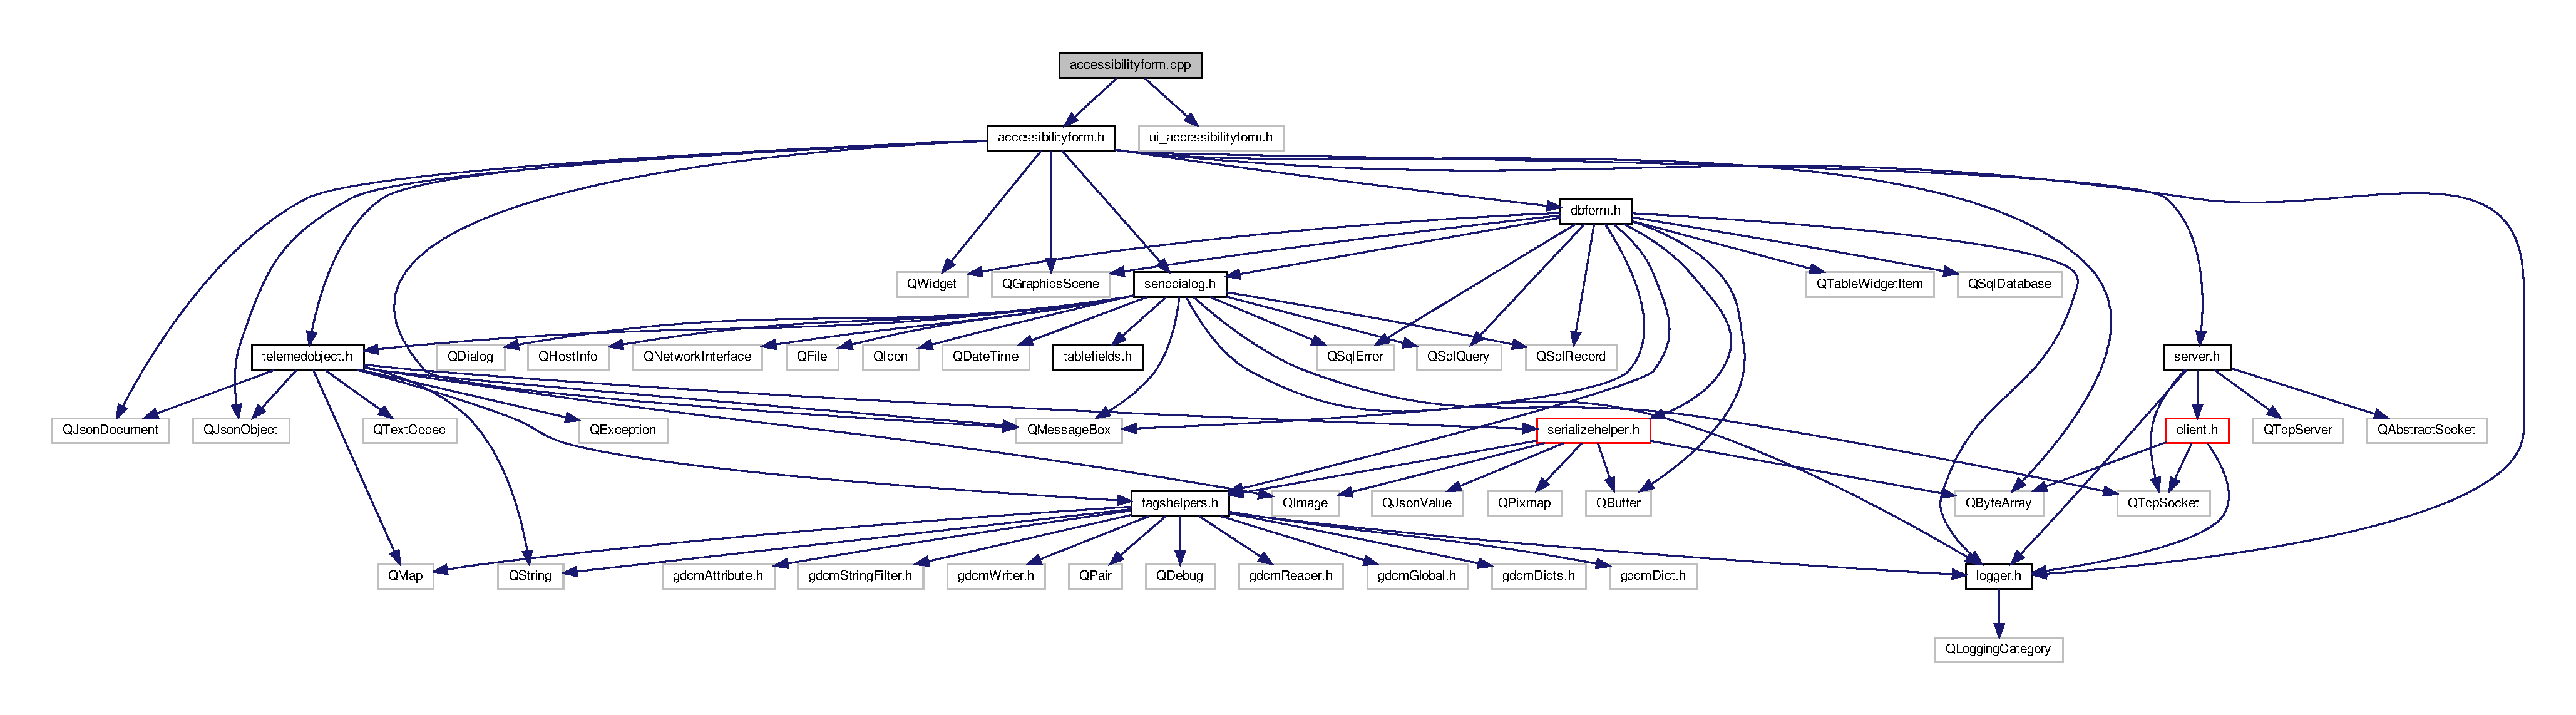
\includegraphics[width=350pt]{accessibilityform_8cpp__incl}
\end{center}
\end{figure}

\hypertarget{accessibilityform_8h}{}\section{Файл accessibilityform.\+h}
\label{accessibilityform_8h}\index{accessibilityform.\+h@{accessibilityform.\+h}}
{\ttfamily \#include $<$Q\+Widget$>$}\newline
{\ttfamily \#include $<$Q\+Json\+Document$>$}\newline
{\ttfamily \#include $<$Q\+Json\+Object$>$}\newline
{\ttfamily \#include $<$Q\+Byte\+Array$>$}\newline
{\ttfamily \#include $<$Q\+Message\+Box$>$}\newline
{\ttfamily \#include $<$Q\+Graphics\+Scene$>$}\newline
{\ttfamily \#include $<$telemedobject.\+h$>$}\newline
{\ttfamily \#include $<$senddialog.\+h$>$}\newline
{\ttfamily \#include $<$logger.\+h$>$}\newline
{\ttfamily \#include \char`\"{}server.\+h\char`\"{}}\newline
{\ttfamily \#include \char`\"{}dbform.\+h\char`\"{}}\newline
Граф включаемых заголовочных файлов для accessibilityform.\+h\+:\nopagebreak
\begin{figure}[H]
\begin{center}
\leavevmode
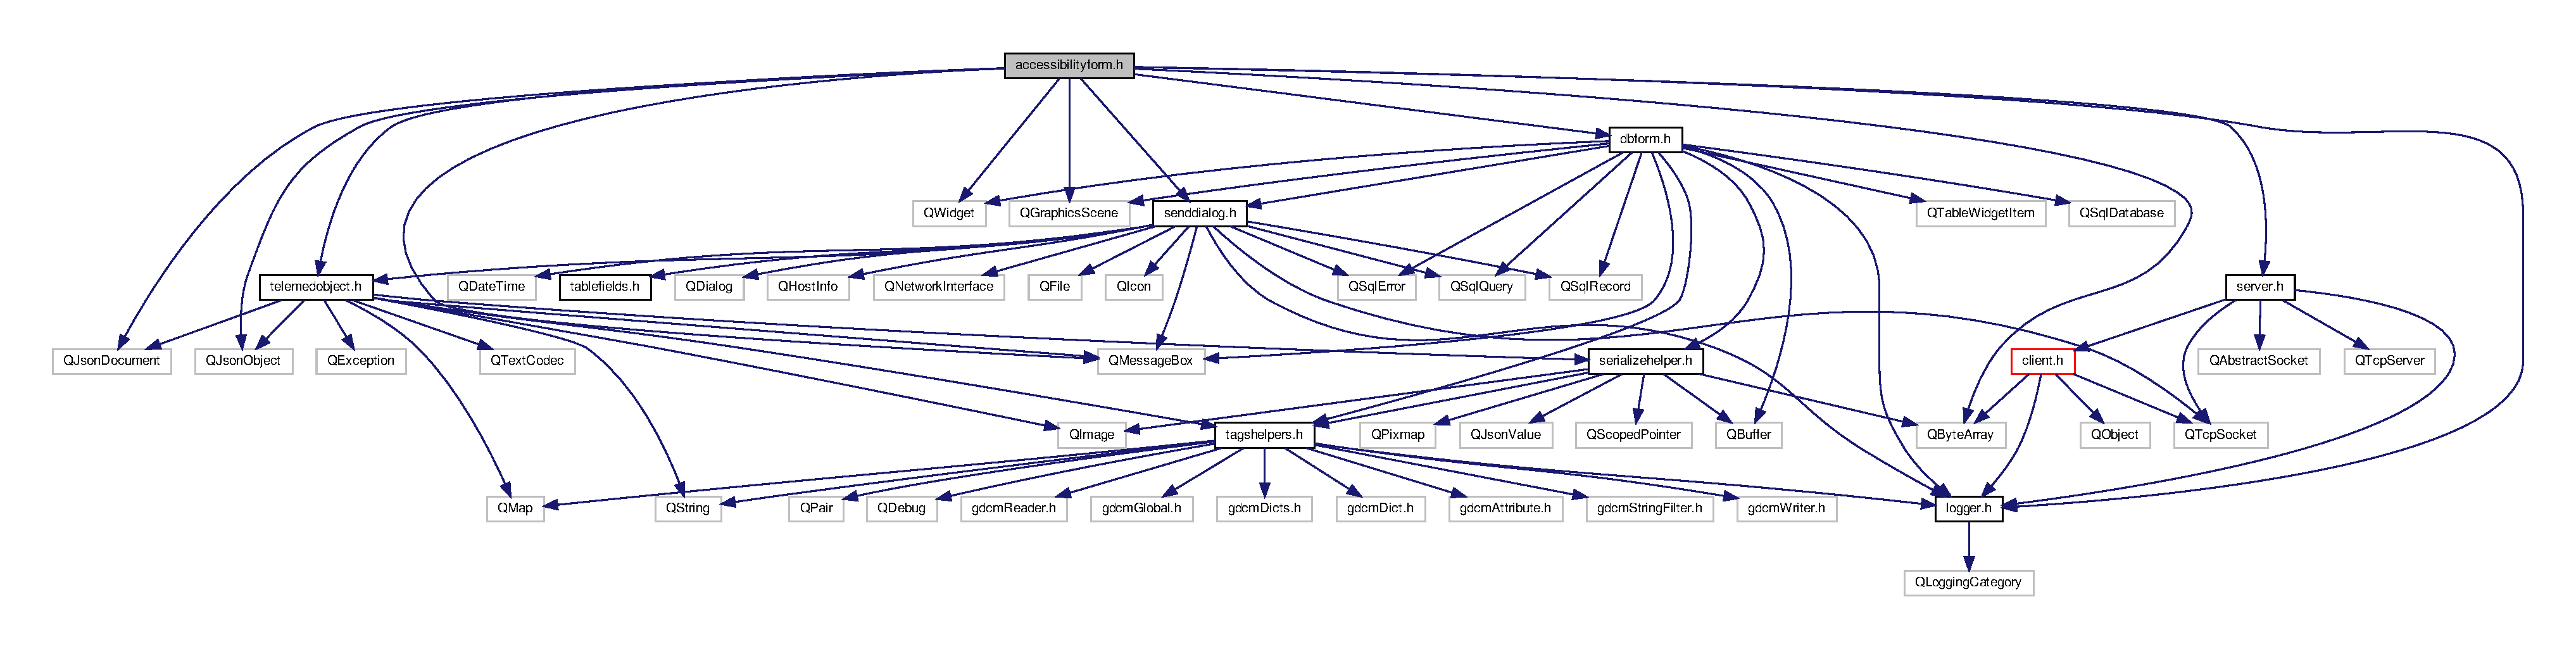
\includegraphics[width=350pt]{accessibilityform_8h__incl}
\end{center}
\end{figure}
Граф файлов, в которые включается этот файл\+:\nopagebreak
\begin{figure}[H]
\begin{center}
\leavevmode
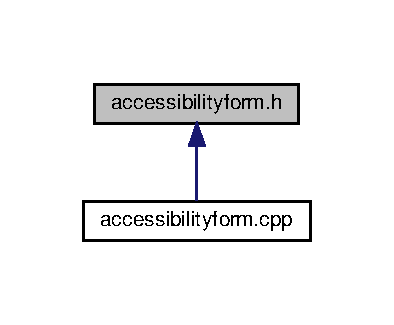
\includegraphics[width=189pt]{accessibilityform_8h__dep__incl}
\end{center}
\end{figure}
\subsection*{Классы}
\begin{DoxyCompactItemize}
\item 
class \hyperlink{classAccessibilityForm}{Accessibility\+Form}
\begin{DoxyCompactList}\small\item\em Класс формы для осуществления сетевого взаимодействия. \end{DoxyCompactList}\end{DoxyCompactItemize}
\subsection*{Пространства имен}
\begin{DoxyCompactItemize}
\item 
 \hyperlink{namespaceUi}{Ui}
\end{DoxyCompactItemize}

\hypertarget{client_8cpp}{}\section{Файл client.\+cpp}
\label{client_8cpp}\index{client.\+cpp@{client.\+cpp}}
{\ttfamily \#include \char`\"{}client.\+h\char`\"{}}\newline
Граф включаемых заголовочных файлов для client.\+cpp\+:\nopagebreak
\begin{figure}[H]
\begin{center}
\leavevmode
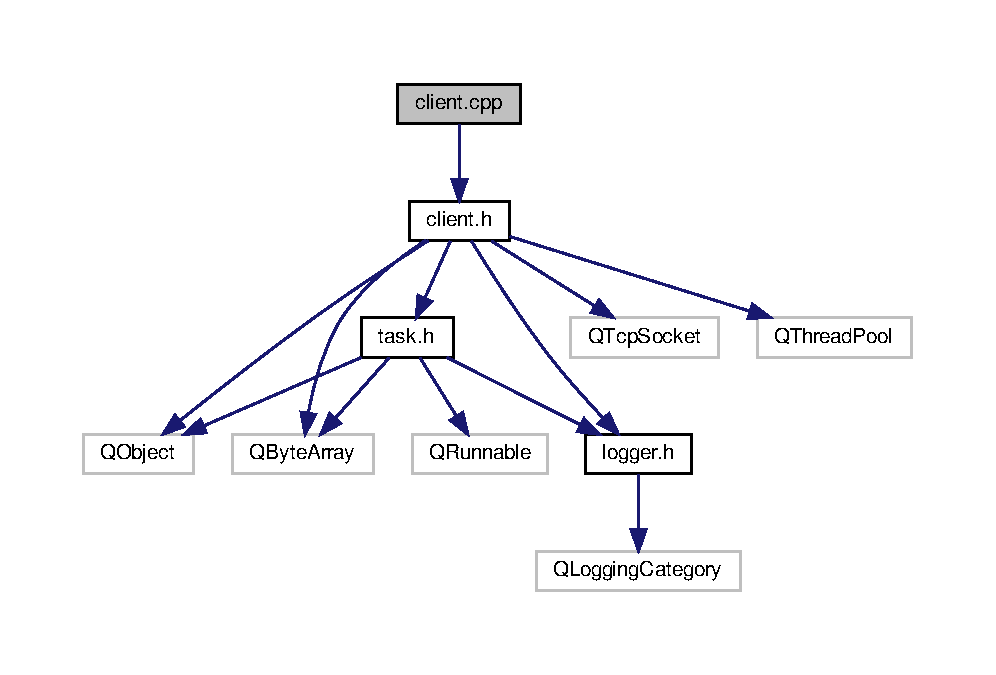
\includegraphics[width=350pt]{client_8cpp__incl}
\end{center}
\end{figure}

\hypertarget{client_8h}{}\section{Файл client.\+h}
\label{client_8h}\index{client.\+h@{client.\+h}}
{\ttfamily \#include $<$Q\+Object$>$}\newline
{\ttfamily \#include $<$Q\+Tcp\+Socket$>$}\newline
{\ttfamily \#include $<$Q\+Thread\+Pool$>$}\newline
{\ttfamily \#include $<$Q\+Byte\+Array$>$}\newline
{\ttfamily \#include $<$logger.\+h$>$}\newline
{\ttfamily \#include $<$task.\+h$>$}\newline
Граф включаемых заголовочных файлов для client.\+h\+:\nopagebreak
\begin{figure}[H]
\begin{center}
\leavevmode
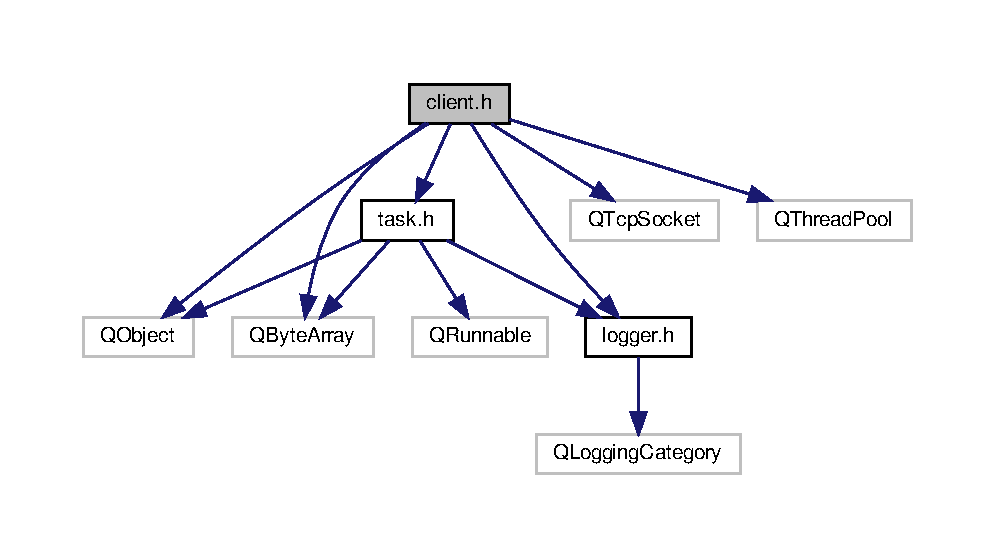
\includegraphics[width=350pt]{client_8h__incl}
\end{center}
\end{figure}
Граф файлов, в которые включается этот файл\+:\nopagebreak
\begin{figure}[H]
\begin{center}
\leavevmode
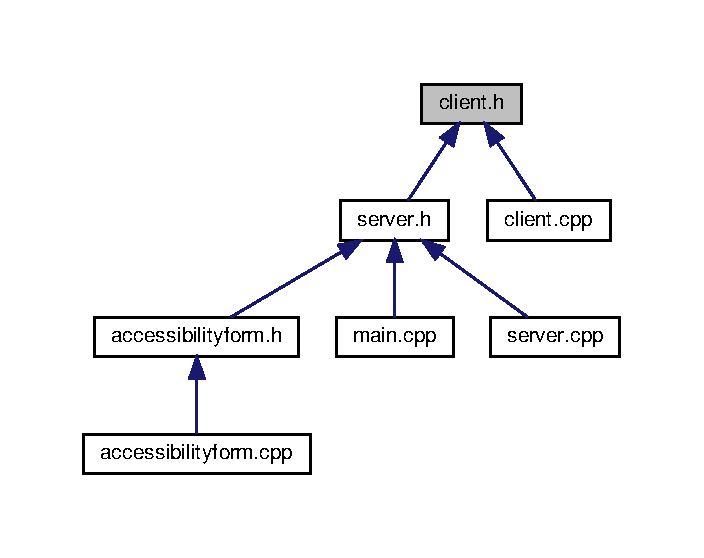
\includegraphics[width=338pt]{client_8h__dep__incl}
\end{center}
\end{figure}
\subsection*{Классы}
\begin{DoxyCompactItemize}
\item 
class \hyperlink{classClient}{Client}
\begin{DoxyCompactList}\small\item\em Класс имитирующий клиента подключенного к серверу \end{DoxyCompactList}\end{DoxyCompactItemize}

\hypertarget{converters_8cpp}{}\section{Файл converters.\+cpp}
\label{converters_8cpp}\index{converters.\+cpp@{converters.\+cpp}}
{\ttfamily \#include $<$converters.\+h$>$}\newline
Граф включаемых заголовочных файлов для converters.\+cpp\+:\nopagebreak
\begin{figure}[H]
\begin{center}
\leavevmode
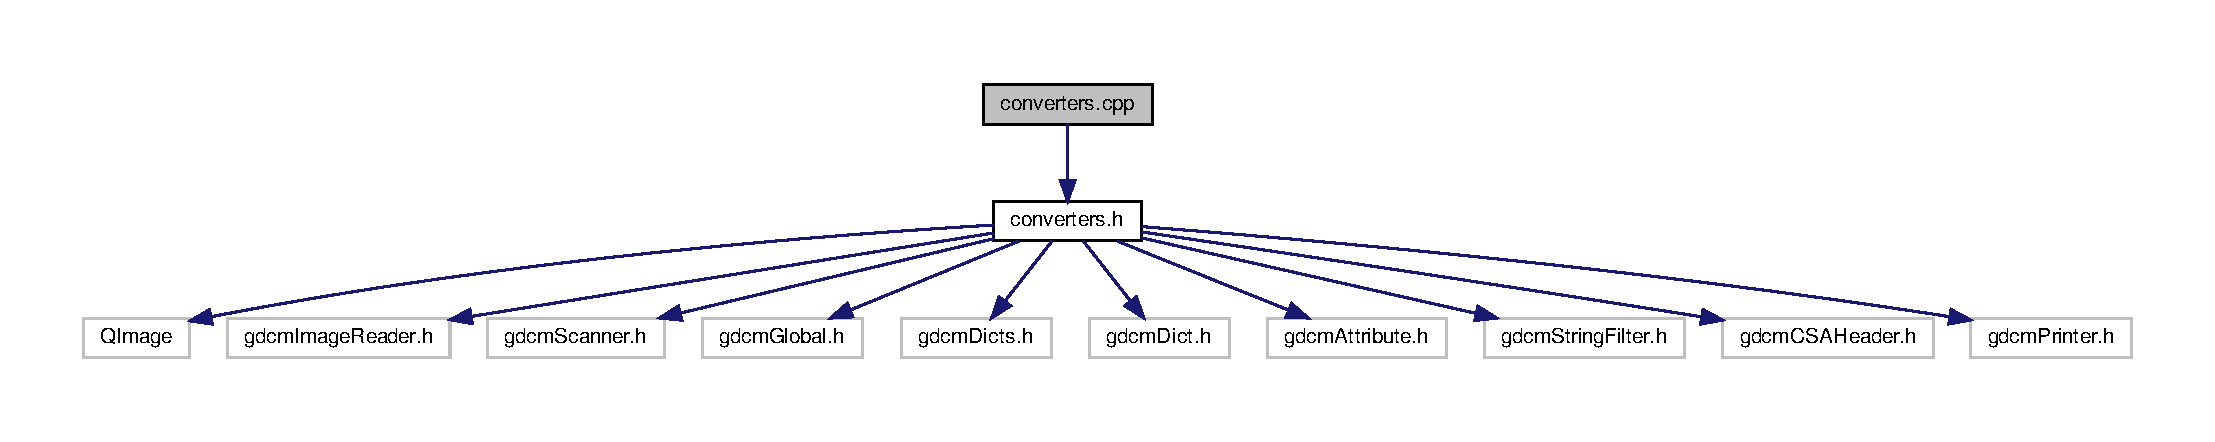
\includegraphics[width=350pt]{converters_8cpp__incl}
\end{center}
\end{figure}
\subsection*{Функции}
\begin{DoxyCompactItemize}
\item 
bool \hyperlink{converters_8cpp_a3cc84957f028460a3f51654587168008}{Convert\+To\+Format\+\_\+\+R\+G\+B888} (gdcm\+::\+Image const \&gimage, char $\ast$buffer, Q\+Image $\ast$\&image\+Qt)
\begin{DoxyCompactList}\small\item\em Функция для конвертации изображения в файле формата dicom в изображение типа Q\+Image. \end{DoxyCompactList}\item 
int \hyperlink{converters_8cpp_a0d3e845f11c48538ab8f45dae9a2d8f3}{Print\+C\+SA} (const std\+::string filename)
\begin{DoxyCompactList}\small\item\em Print\+C\+SA Функция для уведомления о наличии C\+SA тегов. В программе не используется. \end{DoxyCompactList}\end{DoxyCompactItemize}


\subsection{Функции}
\mbox{\Hypertarget{converters_8cpp_a3cc84957f028460a3f51654587168008}\label{converters_8cpp_a3cc84957f028460a3f51654587168008}} 
\index{converters.\+cpp@{converters.\+cpp}!Convert\+To\+Format\+\_\+\+R\+G\+B888@{Convert\+To\+Format\+\_\+\+R\+G\+B888}}
\index{Convert\+To\+Format\+\_\+\+R\+G\+B888@{Convert\+To\+Format\+\_\+\+R\+G\+B888}!converters.\+cpp@{converters.\+cpp}}
\subsubsection{\texorpdfstring{Convert\+To\+Format\+\_\+\+R\+G\+B888()}{ConvertToFormat\_RGB888()}}
{\footnotesize\ttfamily bool Convert\+To\+Format\+\_\+\+R\+G\+B888 (\begin{DoxyParamCaption}\item[{gdcm\+::\+Image const \&}]{gimage,  }\item[{char $\ast$}]{buffer,  }\item[{Q\+Image $\ast$\&}]{image\+Qt }\end{DoxyParamCaption})}



Функция для конвертации изображения в файле формата dicom в изображение типа Q\+Image. 

\mbox{\Hypertarget{converters_8cpp_a0d3e845f11c48538ab8f45dae9a2d8f3}\label{converters_8cpp_a0d3e845f11c48538ab8f45dae9a2d8f3}} 
\index{converters.\+cpp@{converters.\+cpp}!Print\+C\+SA@{Print\+C\+SA}}
\index{Print\+C\+SA@{Print\+C\+SA}!converters.\+cpp@{converters.\+cpp}}
\subsubsection{\texorpdfstring{Print\+C\+S\+A()}{PrintCSA()}}
{\footnotesize\ttfamily int Print\+C\+SA (\begin{DoxyParamCaption}\item[{const std\+::string}]{filename }\end{DoxyParamCaption})}



Print\+C\+SA Функция для уведомления о наличии C\+SA тегов. В программе не используется. 


\begin{DoxyParams}{Аргументы}
{\em filename} & Путь до dicom файла \\
\hline
\end{DoxyParams}
\begin{DoxyReturn}{Возвращает}
1 -\/ если не найдено, 0 -\/ если найдено 
\end{DoxyReturn}

\hypertarget{converters_8h}{}\section{Файл converters.\+h}
\label{converters_8h}\index{converters.\+h@{converters.\+h}}
{\ttfamily \#include $<$Q\+Image$>$}\newline
{\ttfamily \#include \char`\"{}gdcm\+Image\+Reader.\+h\char`\"{}}\newline
{\ttfamily \#include \char`\"{}gdcm\+Scanner.\+h\char`\"{}}\newline
{\ttfamily \#include \char`\"{}gdcm\+Global.\+h\char`\"{}}\newline
{\ttfamily \#include \char`\"{}gdcm\+Dicts.\+h\char`\"{}}\newline
{\ttfamily \#include \char`\"{}gdcm\+Dict.\+h\char`\"{}}\newline
{\ttfamily \#include \char`\"{}gdcm\+Attribute.\+h\char`\"{}}\newline
{\ttfamily \#include \char`\"{}gdcm\+String\+Filter.\+h\char`\"{}}\newline
{\ttfamily \#include \char`\"{}gdcm\+C\+S\+A\+Header.\+h\char`\"{}}\newline
{\ttfamily \#include \char`\"{}gdcm\+Printer.\+h\char`\"{}}\newline
Граф включаемых заголовочных файлов для converters.\+h\+:\nopagebreak
\begin{figure}[H]
\begin{center}
\leavevmode
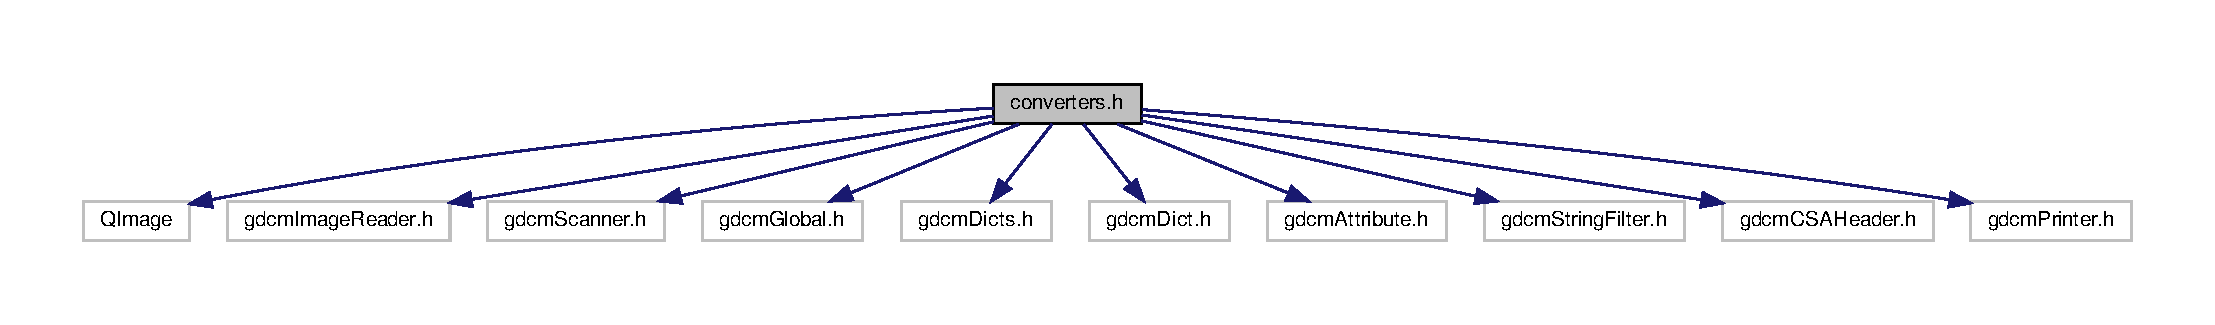
\includegraphics[width=350pt]{converters_8h__incl}
\end{center}
\end{figure}
Граф файлов, в которые включается этот файл\+:\nopagebreak
\begin{figure}[H]
\begin{center}
\leavevmode
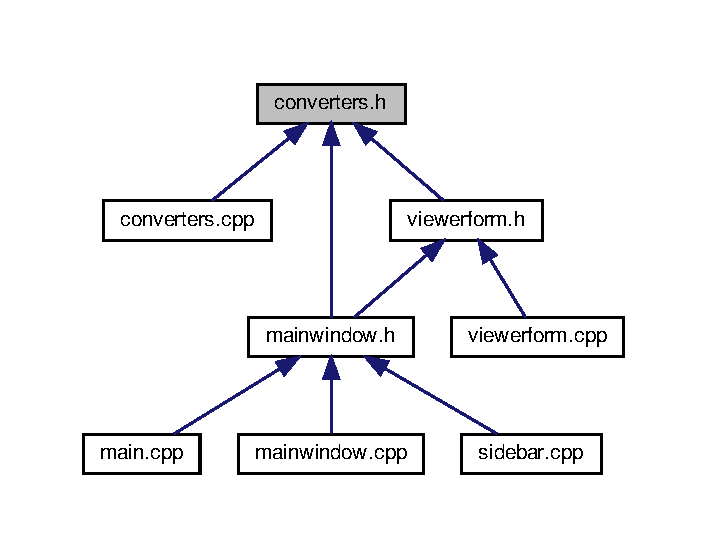
\includegraphics[width=340pt]{converters_8h__dep__incl}
\end{center}
\end{figure}
\subsection*{Функции}
\begin{DoxyCompactItemize}
\item 
bool \hyperlink{converters_8h_a3cc84957f028460a3f51654587168008}{Convert\+To\+Format\+\_\+\+R\+G\+B888} (gdcm\+::\+Image const \&gimage, char $\ast$buffer, Q\+Image $\ast$\&image\+Qt)
\begin{DoxyCompactList}\small\item\em Функция для конвертации изображения в файле формата dicom в изображение типа Q\+Image. \end{DoxyCompactList}\item 
int \hyperlink{converters_8h_a0d3e845f11c48538ab8f45dae9a2d8f3}{Print\+C\+SA} (const std\+::string filename)
\begin{DoxyCompactList}\small\item\em Print\+C\+SA Функция для уведомления о наличии C\+SA тегов. В программе не используется. \end{DoxyCompactList}\end{DoxyCompactItemize}


\subsection{Функции}
\mbox{\Hypertarget{converters_8h_a3cc84957f028460a3f51654587168008}\label{converters_8h_a3cc84957f028460a3f51654587168008}} 
\index{converters.\+h@{converters.\+h}!Convert\+To\+Format\+\_\+\+R\+G\+B888@{Convert\+To\+Format\+\_\+\+R\+G\+B888}}
\index{Convert\+To\+Format\+\_\+\+R\+G\+B888@{Convert\+To\+Format\+\_\+\+R\+G\+B888}!converters.\+h@{converters.\+h}}
\subsubsection{\texorpdfstring{Convert\+To\+Format\+\_\+\+R\+G\+B888()}{ConvertToFormat\_RGB888()}}
{\footnotesize\ttfamily bool Convert\+To\+Format\+\_\+\+R\+G\+B888 (\begin{DoxyParamCaption}\item[{gdcm\+::\+Image const \&}]{gimage,  }\item[{char $\ast$}]{buffer,  }\item[{Q\+Image $\ast$\&}]{image\+Qt }\end{DoxyParamCaption})}



Функция для конвертации изображения в файле формата dicom в изображение типа Q\+Image. 

\mbox{\Hypertarget{converters_8h_a0d3e845f11c48538ab8f45dae9a2d8f3}\label{converters_8h_a0d3e845f11c48538ab8f45dae9a2d8f3}} 
\index{converters.\+h@{converters.\+h}!Print\+C\+SA@{Print\+C\+SA}}
\index{Print\+C\+SA@{Print\+C\+SA}!converters.\+h@{converters.\+h}}
\subsubsection{\texorpdfstring{Print\+C\+S\+A()}{PrintCSA()}}
{\footnotesize\ttfamily int Print\+C\+SA (\begin{DoxyParamCaption}\item[{const std\+::string}]{filename }\end{DoxyParamCaption})}



Print\+C\+SA Функция для уведомления о наличии C\+SA тегов. В программе не используется. 


\begin{DoxyParams}{Аргументы}
{\em filename} & Путь до dicom файла \\
\hline
\end{DoxyParams}
\begin{DoxyReturn}{Возвращает}
1 -\/ если не найдено, 0 -\/ если найдено 
\end{DoxyReturn}

\hypertarget{dbform_8cpp}{}\section{Файл dbform.\+cpp}
\label{dbform_8cpp}\index{dbform.\+cpp@{dbform.\+cpp}}
{\ttfamily \#include \char`\"{}dbform.\+h\char`\"{}}\newline
{\ttfamily \#include \char`\"{}ui\+\_\+dbform.\+h\char`\"{}}\newline
Граф включаемых заголовочных файлов для dbform.\+cpp\+:\nopagebreak
\begin{figure}[H]
\begin{center}
\leavevmode
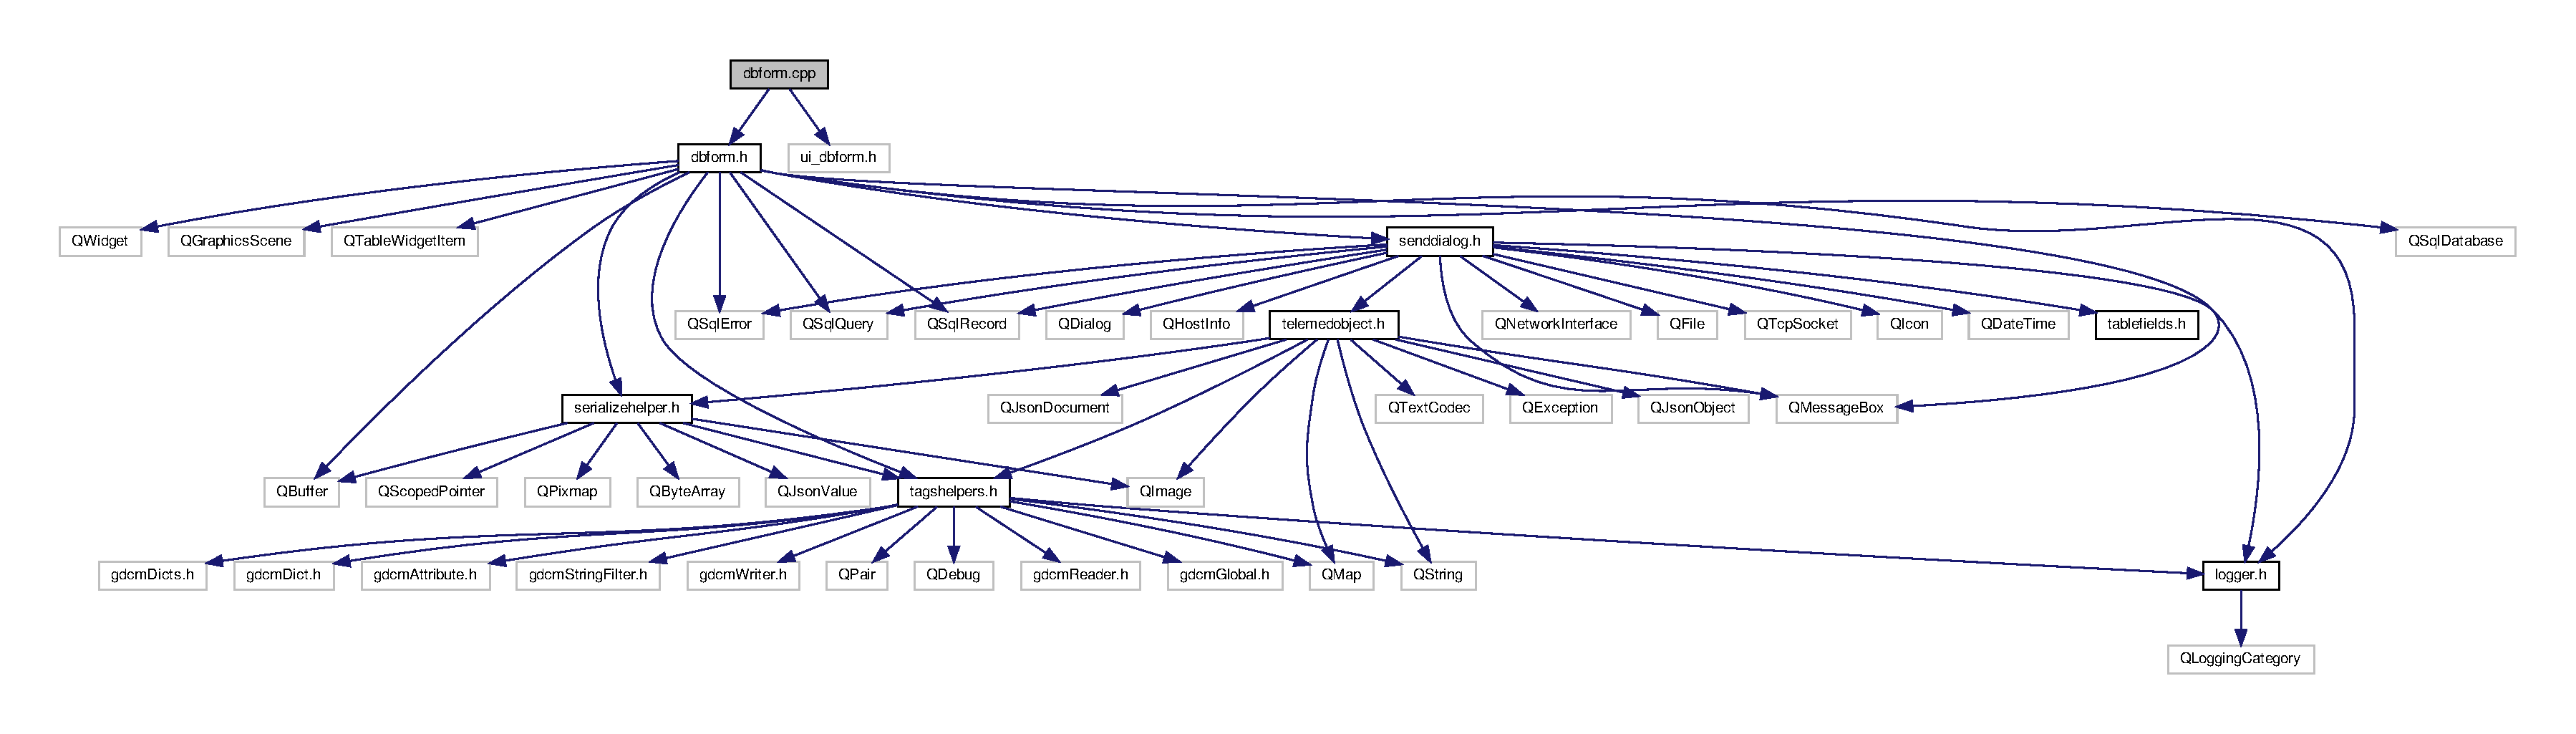
\includegraphics[width=350pt]{dbform_8cpp__incl}
\end{center}
\end{figure}

\hypertarget{dbform_8h}{}\section{Файл dbform.\+h}
\label{dbform_8h}\index{dbform.\+h@{dbform.\+h}}
{\ttfamily \#include $<$Q\+Widget$>$}\newline
{\ttfamily \#include $<$Q\+Graphics\+Scene$>$}\newline
{\ttfamily \#include $<$Q\+Table\+Widget\+Item$>$}\newline
{\ttfamily \#include $<$Q\+Buffer$>$}\newline
{\ttfamily \#include $<$Q\+Sql\+Error$>$}\newline
{\ttfamily \#include $<$Q\+Sql\+Database$>$}\newline
{\ttfamily \#include $<$Q\+Message\+Box$>$}\newline
{\ttfamily \#include $<$Q\+Sql\+Query$>$}\newline
{\ttfamily \#include $<$Q\+Sql\+Record$>$}\newline
{\ttfamily \#include $<$logger.\+h$>$}\newline
{\ttfamily \#include $<$tagshelpers.\+h$>$}\newline
{\ttfamily \#include $<$serializehelper.\+h$>$}\newline
{\ttfamily \#include \char`\"{}senddialog.\+h\char`\"{}}\newline
Граф включаемых заголовочных файлов для dbform.\+h\+:\nopagebreak
\begin{figure}[H]
\begin{center}
\leavevmode
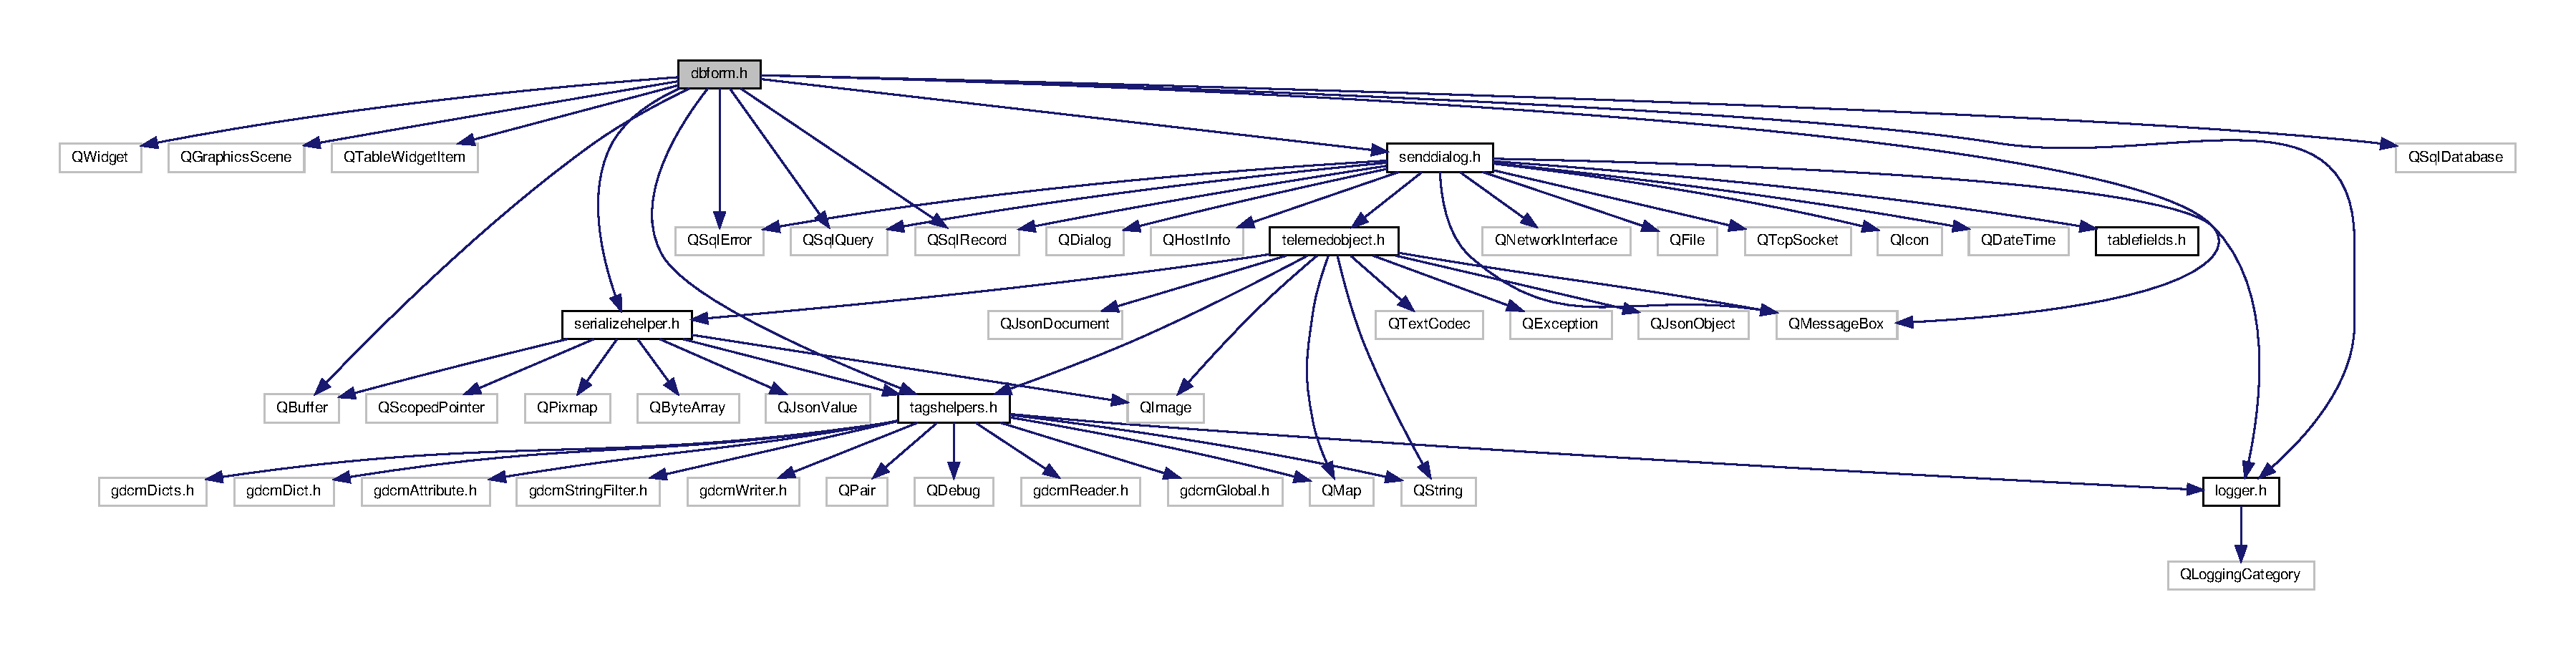
\includegraphics[width=350pt]{dbform_8h__incl}
\end{center}
\end{figure}
Граф файлов, в которые включается этот файл\+:\nopagebreak
\begin{figure}[H]
\begin{center}
\leavevmode
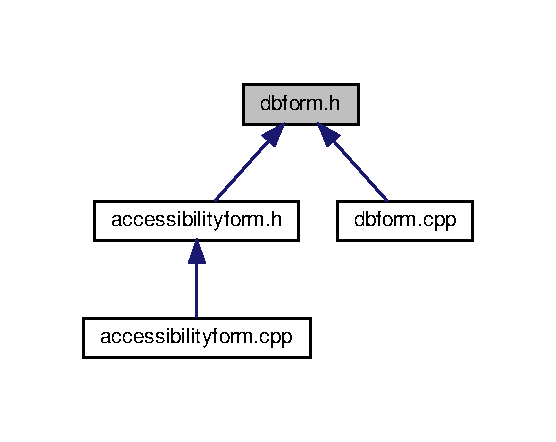
\includegraphics[width=267pt]{dbform_8h__dep__incl}
\end{center}
\end{figure}
\subsection*{Классы}
\begin{DoxyCompactItemize}
\item 
class \hyperlink{classDbForm}{Db\+Form}
\begin{DoxyCompactList}\small\item\em Класс формы для отображения содержимого базы данных \end{DoxyCompactList}\end{DoxyCompactItemize}
\subsection*{Пространства имен}
\begin{DoxyCompactItemize}
\item 
 \hyperlink{namespaceUi}{Ui}
\end{DoxyCompactItemize}
\subsection*{Определения типов}
\begin{DoxyCompactItemize}
\item 
using \hyperlink{dbform_8h_a1ec1a645f41e1c6544d384ca863a936c}{add\+Info\+Map} = Q\+Map$<$ Q\+String, Q\+String $>$
\end{DoxyCompactItemize}


\subsection{Типы}
\mbox{\Hypertarget{dbform_8h_a1ec1a645f41e1c6544d384ca863a936c}\label{dbform_8h_a1ec1a645f41e1c6544d384ca863a936c}} 
\index{dbform.\+h@{dbform.\+h}!add\+Info\+Map@{add\+Info\+Map}}
\index{add\+Info\+Map@{add\+Info\+Map}!dbform.\+h@{dbform.\+h}}
\subsubsection{\texorpdfstring{add\+Info\+Map}{addInfoMap}}
{\footnotesize\ttfamily using \hyperlink{dbform_8h_a1ec1a645f41e1c6544d384ca863a936c}{add\+Info\+Map} =  Q\+Map$<$Q\+String,Q\+String$>$}


\hypertarget{logger_8cpp}{}\section{Файл logger.\+cpp}
\label{logger_8cpp}\index{logger.\+cpp@{logger.\+cpp}}
{\ttfamily \#include $<$logger.\+h$>$}\newline
Граф включаемых заголовочных файлов для logger.\+cpp\+:\nopagebreak
\begin{figure}[H]
\begin{center}
\leavevmode
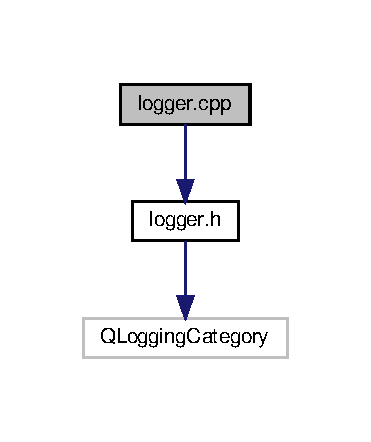
\includegraphics[width=178pt]{logger_8cpp__incl}
\end{center}
\end{figure}

\hypertarget{logger_8h}{}\section{Файл logger.\+h}
\label{logger_8h}\index{logger.\+h@{logger.\+h}}
{\ttfamily \#include $<$Q\+Logging\+Category$>$}\newline
Граф включаемых заголовочных файлов для logger.\+h\+:\nopagebreak
\begin{figure}[H]
\begin{center}
\leavevmode
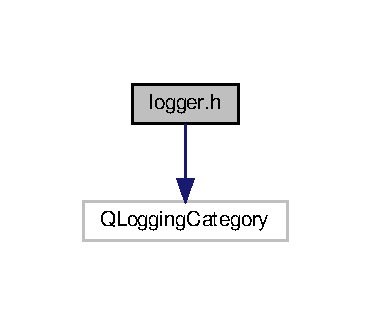
\includegraphics[width=178pt]{logger_8h__incl}
\end{center}
\end{figure}
Граф файлов, в которые включается этот файл\+:\nopagebreak
\begin{figure}[H]
\begin{center}
\leavevmode
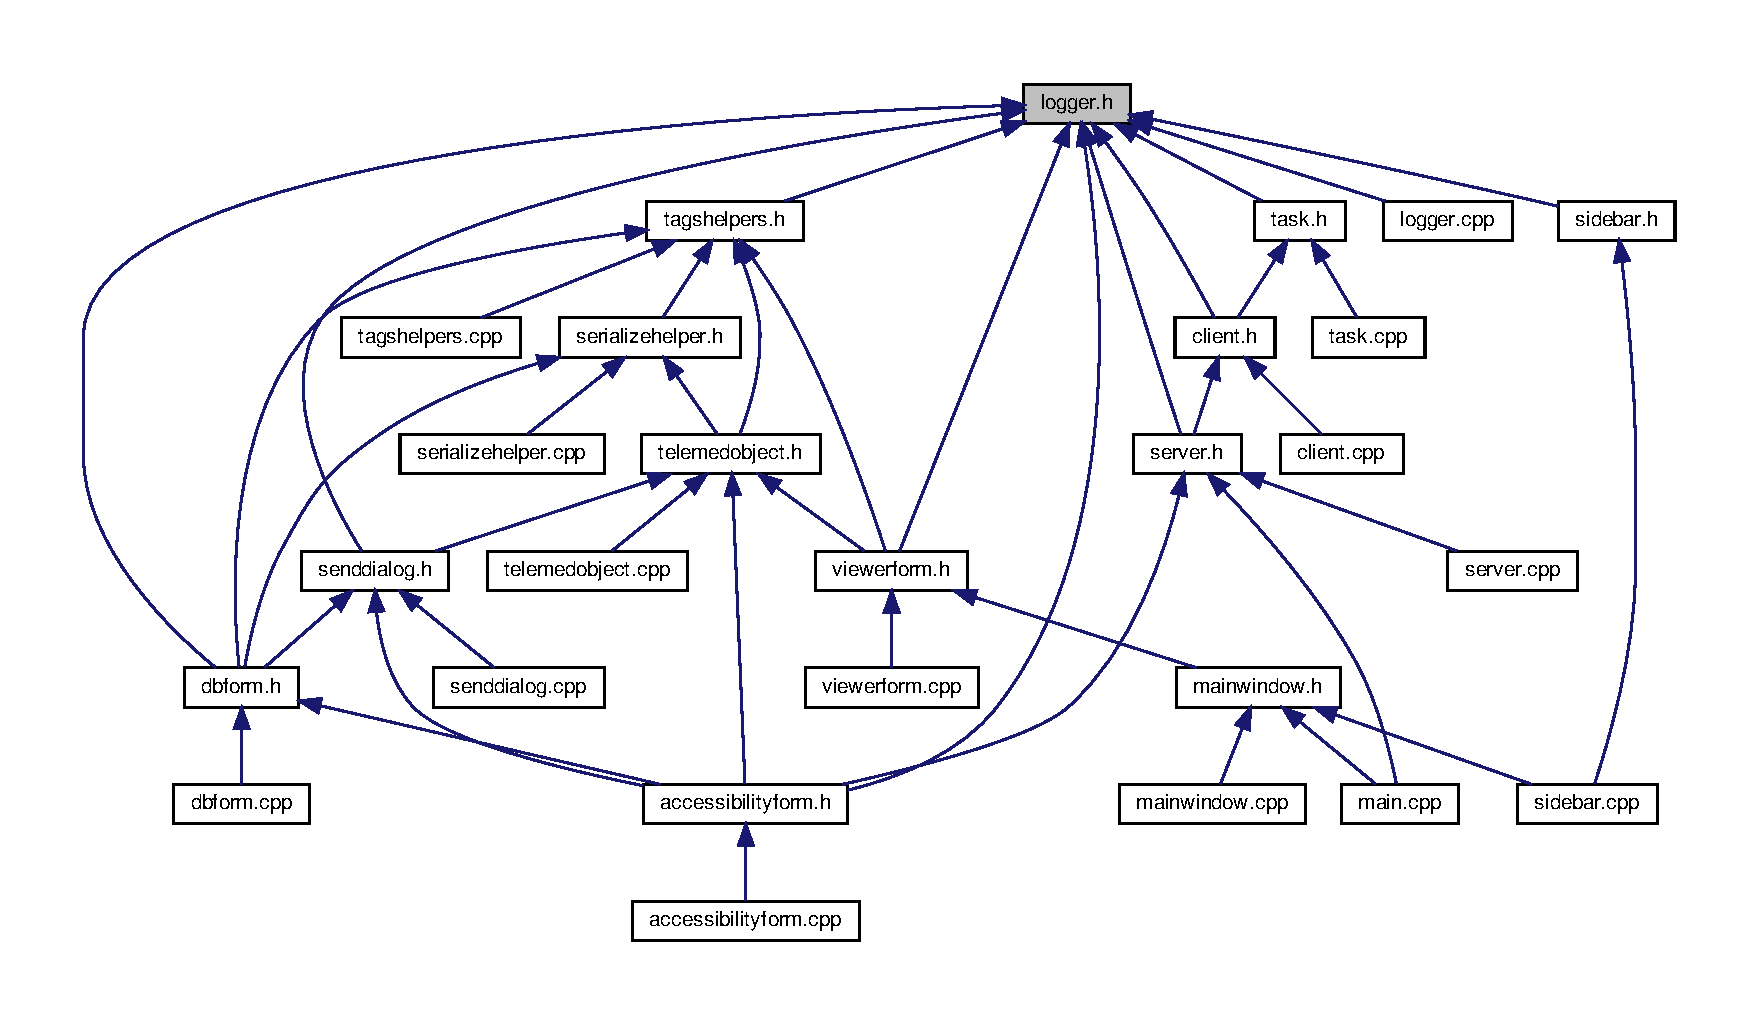
\includegraphics[width=350pt]{logger_8h__dep__incl}
\end{center}
\end{figure}

\hypertarget{main_8cpp}{}\section{Файл main.\+cpp}
\label{main_8cpp}\index{main.\+cpp@{main.\+cpp}}
{\ttfamily \#include \char`\"{}mainwindow.\+h\char`\"{}}\newline
{\ttfamily \#include $<$Q\+Application$>$}\newline
{\ttfamily \#include $<$Q\+System\+Semaphore$>$}\newline
{\ttfamily \#include $<$Q\+Shared\+Memory$>$}\newline
{\ttfamily \#include $<$Q\+Scoped\+Pointer$>$}\newline
{\ttfamily \#include $<$Q\+File$>$}\newline
{\ttfamily \#include $<$Q\+Logging\+Category$>$}\newline
{\ttfamily \#include $<$Q\+Date\+Time$>$}\newline
{\ttfamily \#include $<$Q\+Text\+Stream$>$}\newline
{\ttfamily \#include \char`\"{}server.\+h\char`\"{}}\newline
Граф включаемых заголовочных файлов для main.\+cpp\+:\nopagebreak
\begin{figure}[H]
\begin{center}
\leavevmode
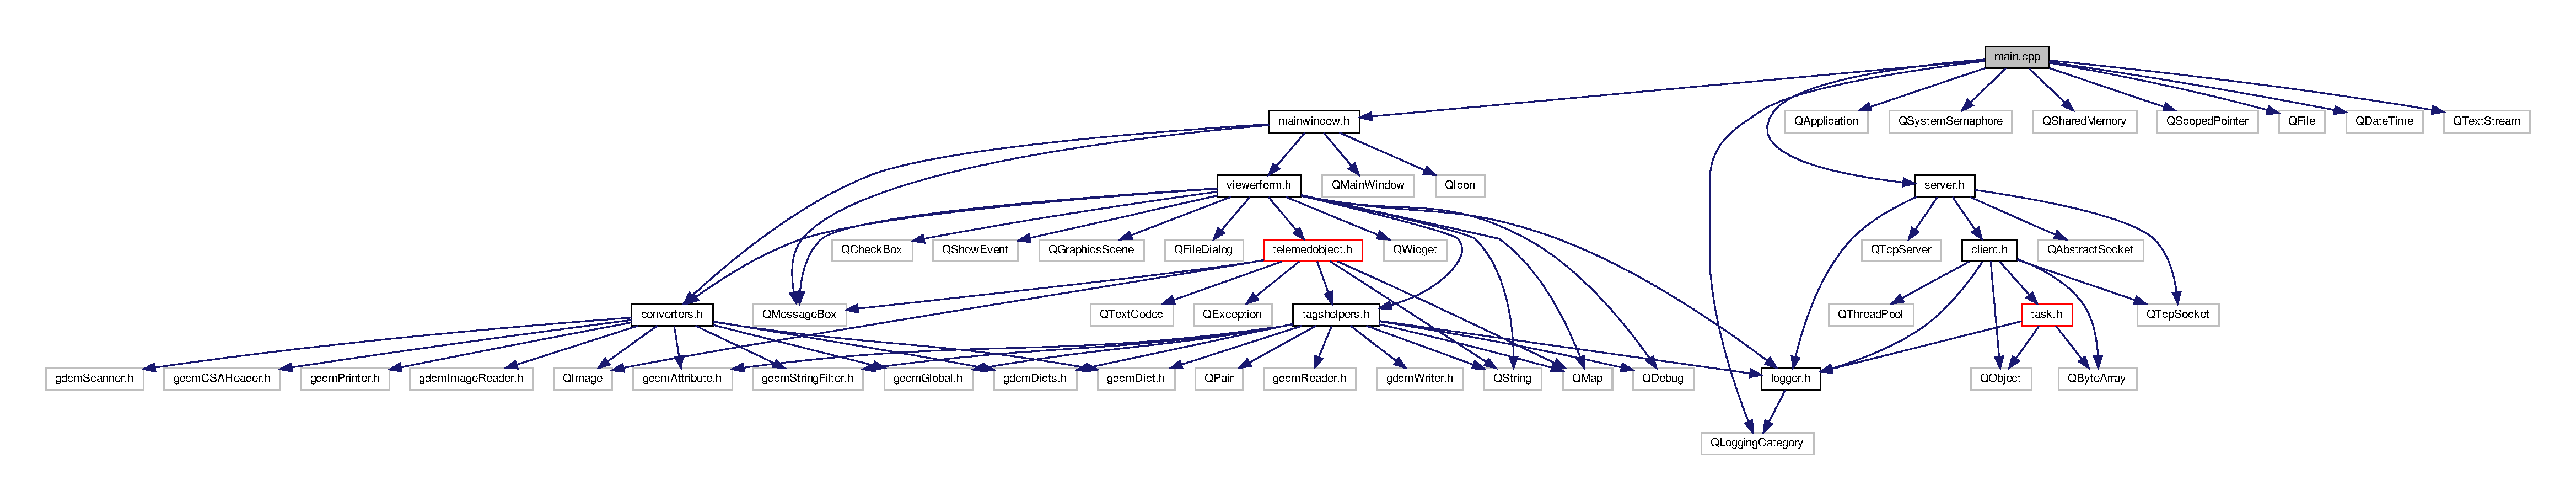
\includegraphics[width=350pt]{main_8cpp__incl}
\end{center}
\end{figure}
\subsection*{Функции}
\begin{DoxyCompactItemize}
\item 
void \hyperlink{main_8cpp_a9606ad1b9a909a366a2d8317438d2e58}{message\+Handler} (Qt\+Msg\+Type type, const Q\+Message\+Log\+Context \&context, const Q\+String \&msg)
\item 
int \hyperlink{main_8cpp_a0ddf1224851353fc92bfbff6f499fa97}{main} (int argc, char $\ast$argv\mbox{[}$\,$\mbox{]})
\end{DoxyCompactItemize}


\subsection{Функции}
\mbox{\Hypertarget{main_8cpp_a0ddf1224851353fc92bfbff6f499fa97}\label{main_8cpp_a0ddf1224851353fc92bfbff6f499fa97}} 
\index{main.\+cpp@{main.\+cpp}!main@{main}}
\index{main@{main}!main.\+cpp@{main.\+cpp}}
\subsubsection{\texorpdfstring{main()}{main()}}
{\footnotesize\ttfamily int main (\begin{DoxyParamCaption}\item[{int}]{argc,  }\item[{char $\ast$}]{argv\mbox{[}$\,$\mbox{]} }\end{DoxyParamCaption})}

\mbox{\Hypertarget{main_8cpp_a9606ad1b9a909a366a2d8317438d2e58}\label{main_8cpp_a9606ad1b9a909a366a2d8317438d2e58}} 
\index{main.\+cpp@{main.\+cpp}!message\+Handler@{message\+Handler}}
\index{message\+Handler@{message\+Handler}!main.\+cpp@{main.\+cpp}}
\subsubsection{\texorpdfstring{message\+Handler()}{messageHandler()}}
{\footnotesize\ttfamily void message\+Handler (\begin{DoxyParamCaption}\item[{Qt\+Msg\+Type}]{type,  }\item[{const Q\+Message\+Log\+Context \&}]{context,  }\item[{const Q\+String \&}]{msg }\end{DoxyParamCaption})}


\hypertarget{mainwindow_8cpp}{}\section{Файл mainwindow.\+cpp}
\label{mainwindow_8cpp}\index{mainwindow.\+cpp@{mainwindow.\+cpp}}
{\ttfamily \#include \char`\"{}mainwindow.\+h\char`\"{}}\newline
{\ttfamily \#include \char`\"{}ui\+\_\+mainwindow.\+h\char`\"{}}\newline
Граф включаемых заголовочных файлов для mainwindow.\+cpp\+:\nopagebreak
\begin{figure}[H]
\begin{center}
\leavevmode
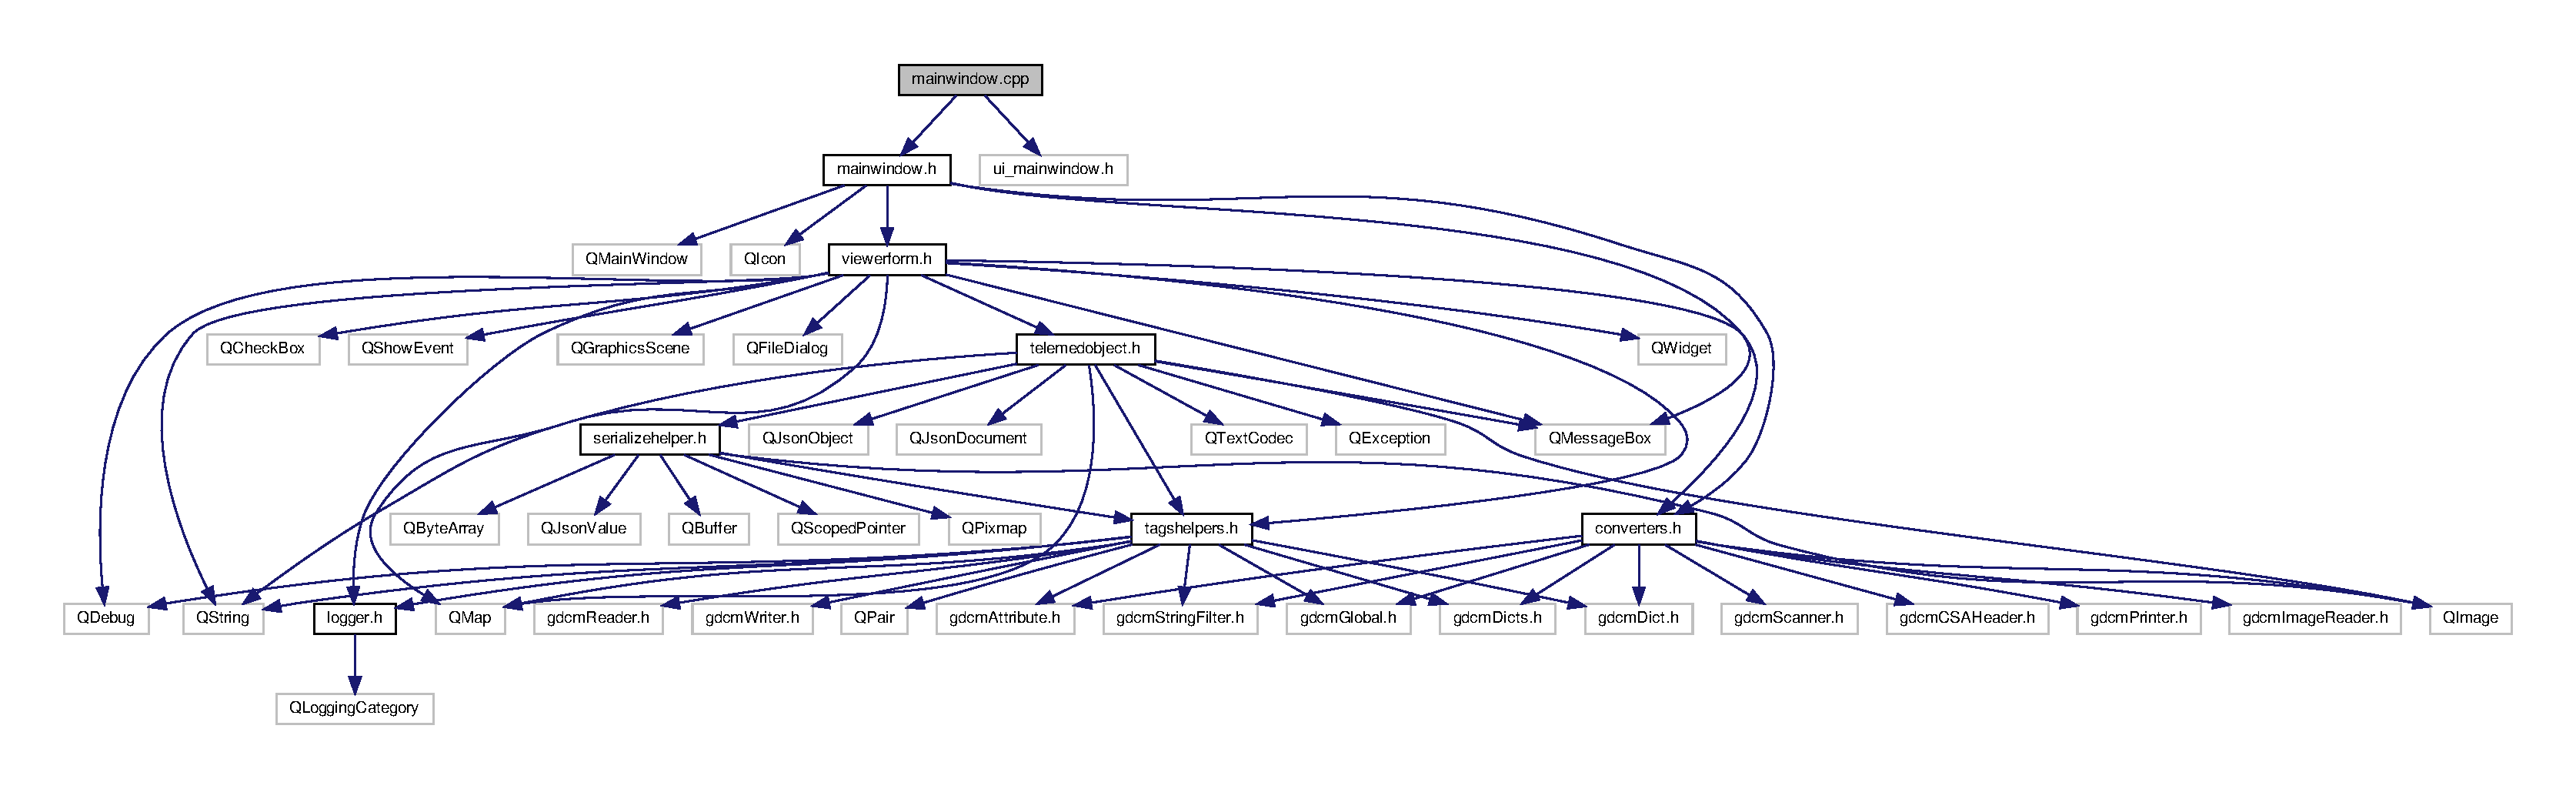
\includegraphics[width=350pt]{mainwindow_8cpp__incl}
\end{center}
\end{figure}

\hypertarget{mainwindow_8h}{}\section{Файл mainwindow.\+h}
\label{mainwindow_8h}\index{mainwindow.\+h@{mainwindow.\+h}}
{\ttfamily \#include $<$Q\+Main\+Window$>$}\newline
{\ttfamily \#include $<$Q\+Icon$>$}\newline
{\ttfamily \#include $<$Q\+Message\+Box$>$}\newline
{\ttfamily \#include $<$viewerform.\+h$>$}\newline
{\ttfamily \#include $<$converters.\+h$>$}\newline
Граф включаемых заголовочных файлов для mainwindow.\+h\+:\nopagebreak
\begin{figure}[H]
\begin{center}
\leavevmode
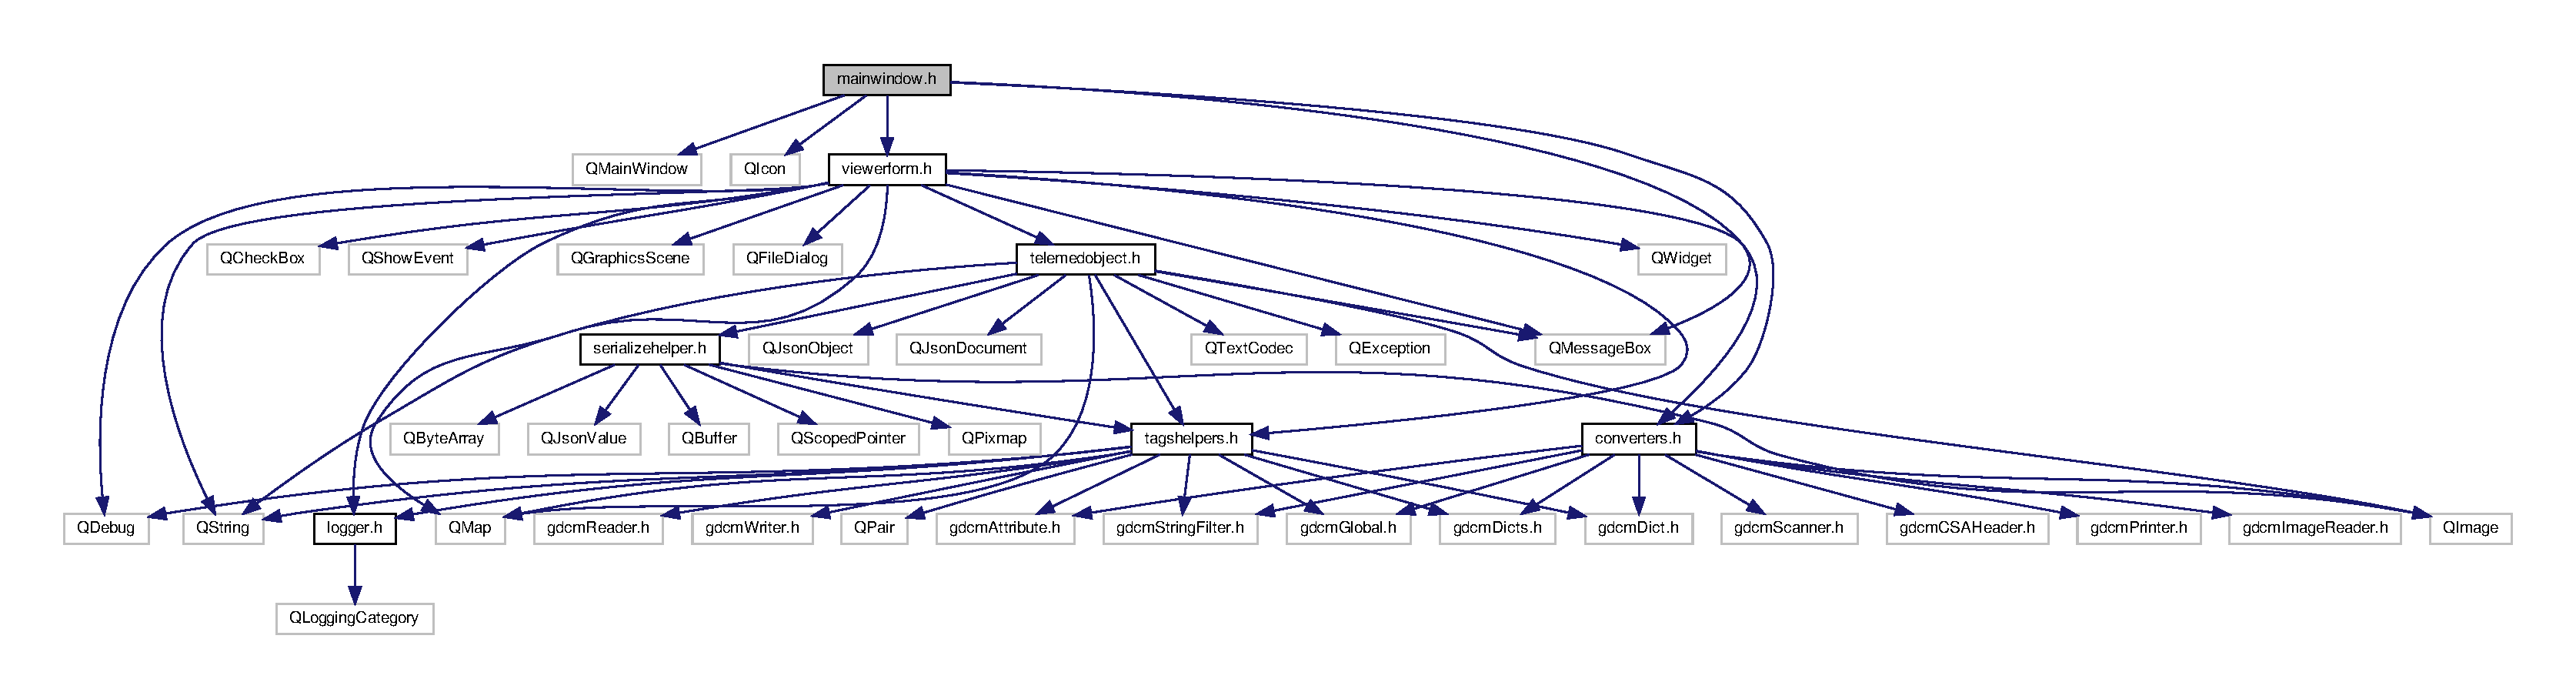
\includegraphics[width=350pt]{mainwindow_8h__incl}
\end{center}
\end{figure}
Граф файлов, в которые включается этот файл\+:\nopagebreak
\begin{figure}[H]
\begin{center}
\leavevmode
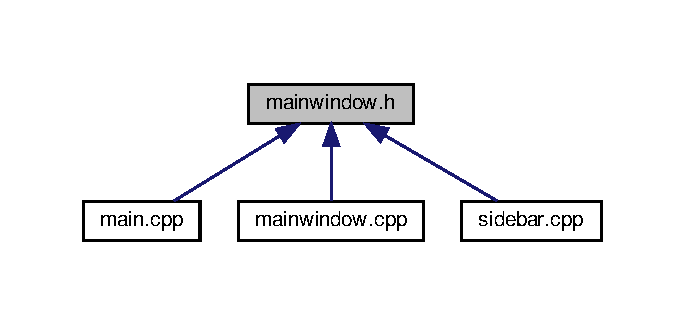
\includegraphics[width=329pt]{mainwindow_8h__dep__incl}
\end{center}
\end{figure}
\subsection*{Классы}
\begin{DoxyCompactItemize}
\item 
class \hyperlink{classMainWindow}{Main\+Window}
\begin{DoxyCompactList}\small\item\em Класс главного окна программы. \end{DoxyCompactList}\end{DoxyCompactItemize}
\subsection*{Пространства имен}
\begin{DoxyCompactItemize}
\item 
 \hyperlink{namespaceUi}{Ui}
\end{DoxyCompactItemize}
\subsection*{Определения типов}
\begin{DoxyCompactItemize}
\item 
using \hyperlink{mainwindow_8h_a8865f4251cec2170c8651965cbb8d5da}{add\+Info\+Map} = Q\+Map$<$ Q\+String, Q\+String $>$
\end{DoxyCompactItemize}


\subsection{Типы}
\mbox{\Hypertarget{mainwindow_8h_a8865f4251cec2170c8651965cbb8d5da}\label{mainwindow_8h_a8865f4251cec2170c8651965cbb8d5da}} 
\index{mainwindow.\+h@{mainwindow.\+h}!add\+Info\+Map@{add\+Info\+Map}}
\index{add\+Info\+Map@{add\+Info\+Map}!mainwindow.\+h@{mainwindow.\+h}}
\subsubsection{\texorpdfstring{add\+Info\+Map}{addInfoMap}}
{\footnotesize\ttfamily using \hyperlink{dbform_8h_a1ec1a645f41e1c6544d384ca863a936c}{add\+Info\+Map} =  Q\+Map$<$Q\+String, Q\+String$>$}


\hypertarget{scenezoom_8cpp}{}\section{Файл scenezoom.\+cpp}
\label{scenezoom_8cpp}\index{scenezoom.\+cpp@{scenezoom.\+cpp}}
{\ttfamily \#include \char`\"{}scenezoom.\+h\char`\"{}}\newline
Граф включаемых заголовочных файлов для scenezoom.\+cpp\+:\nopagebreak
\begin{figure}[H]
\begin{center}
\leavevmode
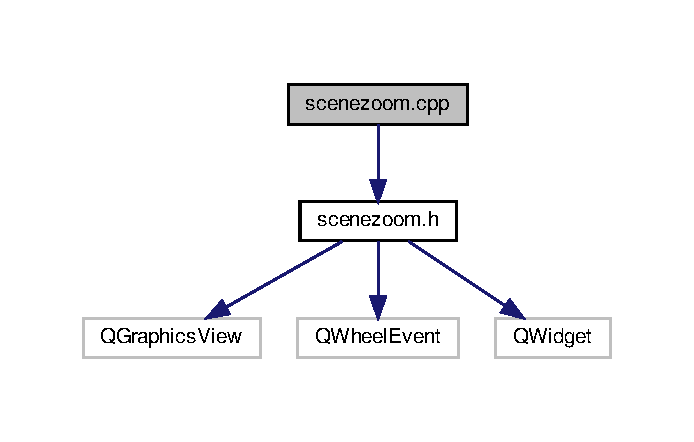
\includegraphics[width=333pt]{scenezoom_8cpp__incl}
\end{center}
\end{figure}

\hypertarget{scenezoom_8h}{}\section{Файл scenezoom.\+h}
\label{scenezoom_8h}\index{scenezoom.\+h@{scenezoom.\+h}}
{\ttfamily \#include $<$Q\+Graphics\+View$>$}\newline
{\ttfamily \#include $<$Q\+Wheel\+Event$>$}\newline
{\ttfamily \#include $<$Q\+Widget$>$}\newline
Граф включаемых заголовочных файлов для scenezoom.\+h\+:\nopagebreak
\begin{figure}[H]
\begin{center}
\leavevmode
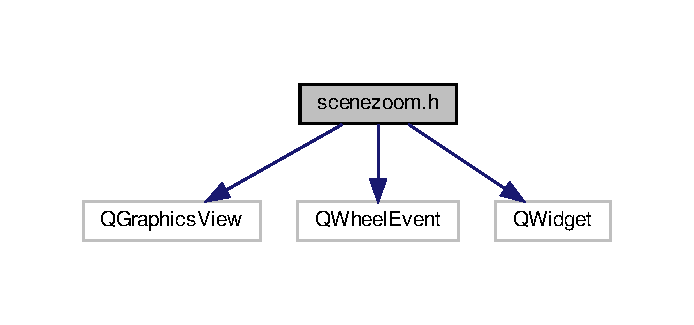
\includegraphics[width=333pt]{scenezoom_8h__incl}
\end{center}
\end{figure}
Граф файлов, в которые включается этот файл\+:\nopagebreak
\begin{figure}[H]
\begin{center}
\leavevmode
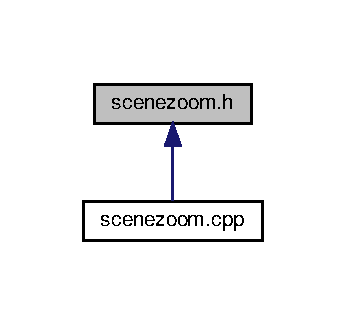
\includegraphics[width=166pt]{scenezoom_8h__dep__incl}
\end{center}
\end{figure}
\subsection*{Классы}
\begin{DoxyCompactItemize}
\item 
class \hyperlink{classSceneZoom}{Scene\+Zoom}
\begin{DoxyCompactList}\small\item\em Класс реализующий логику зумирования изображения в сцене на виджете \end{DoxyCompactList}\end{DoxyCompactItemize}

\hypertarget{senddialog_8cpp}{}\section{Файл senddialog.\+cpp}
\label{senddialog_8cpp}\index{senddialog.\+cpp@{senddialog.\+cpp}}
{\ttfamily \#include \char`\"{}senddialog.\+h\char`\"{}}\newline
{\ttfamily \#include \char`\"{}ui\+\_\+senddialog.\+h\char`\"{}}\newline
Граф включаемых заголовочных файлов для senddialog.\+cpp\+:\nopagebreak
\begin{figure}[H]
\begin{center}
\leavevmode
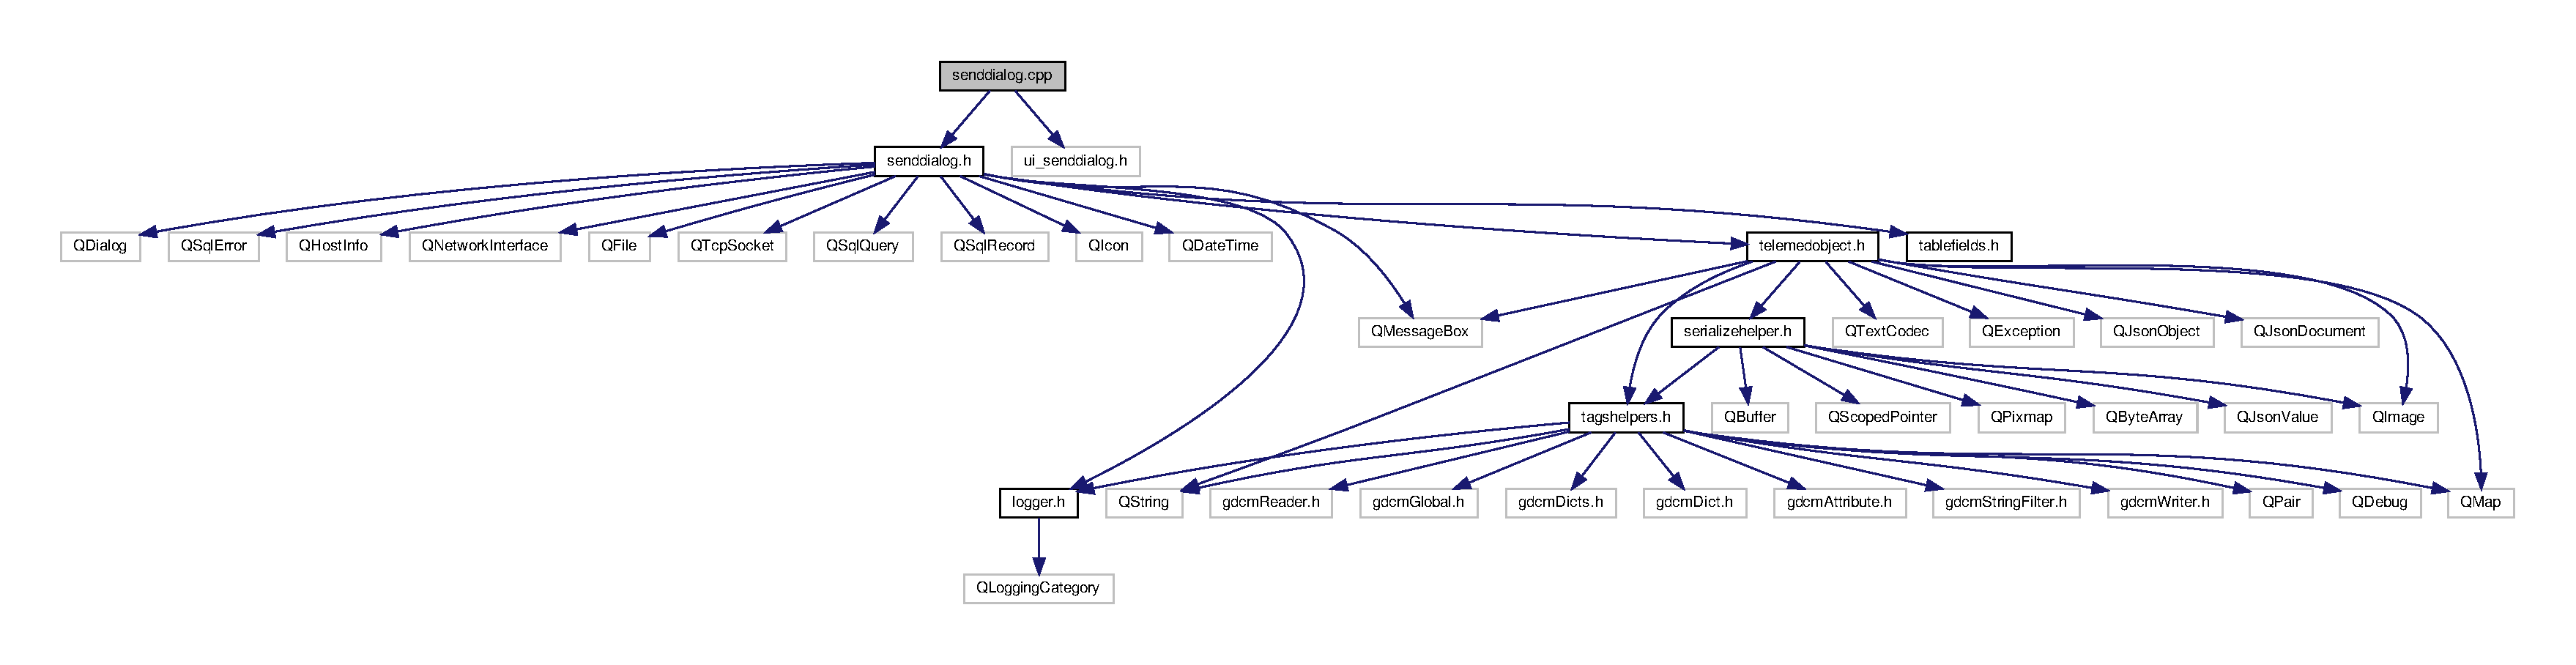
\includegraphics[width=350pt]{senddialog_8cpp__incl}
\end{center}
\end{figure}

\hypertarget{senddialog_8h}{}\section{Файл senddialog.\+h}
\label{senddialog_8h}\index{senddialog.\+h@{senddialog.\+h}}
{\ttfamily \#include $<$Q\+Dialog$>$}\newline
{\ttfamily \#include $<$Q\+Sql\+Error$>$}\newline
{\ttfamily \#include $<$Q\+Host\+Info$>$}\newline
{\ttfamily \#include $<$Q\+Network\+Interface$>$}\newline
{\ttfamily \#include $<$Q\+File$>$}\newline
{\ttfamily \#include $<$Q\+Tcp\+Socket$>$}\newline
{\ttfamily \#include $<$Q\+Sql\+Query$>$}\newline
{\ttfamily \#include $<$Q\+Sql\+Record$>$}\newline
{\ttfamily \#include $<$Q\+Icon$>$}\newline
{\ttfamily \#include $<$Q\+Date\+Time$>$}\newline
{\ttfamily \#include $<$Q\+Message\+Box$>$}\newline
{\ttfamily \#include \char`\"{}logger.\+h\char`\"{}}\newline
{\ttfamily \#include \char`\"{}telemedobject.\+h\char`\"{}}\newline
{\ttfamily \#include \char`\"{}tablefields.\+h\char`\"{}}\newline
Граф включаемых заголовочных файлов для senddialog.\+h\+:\nopagebreak
\begin{figure}[H]
\begin{center}
\leavevmode
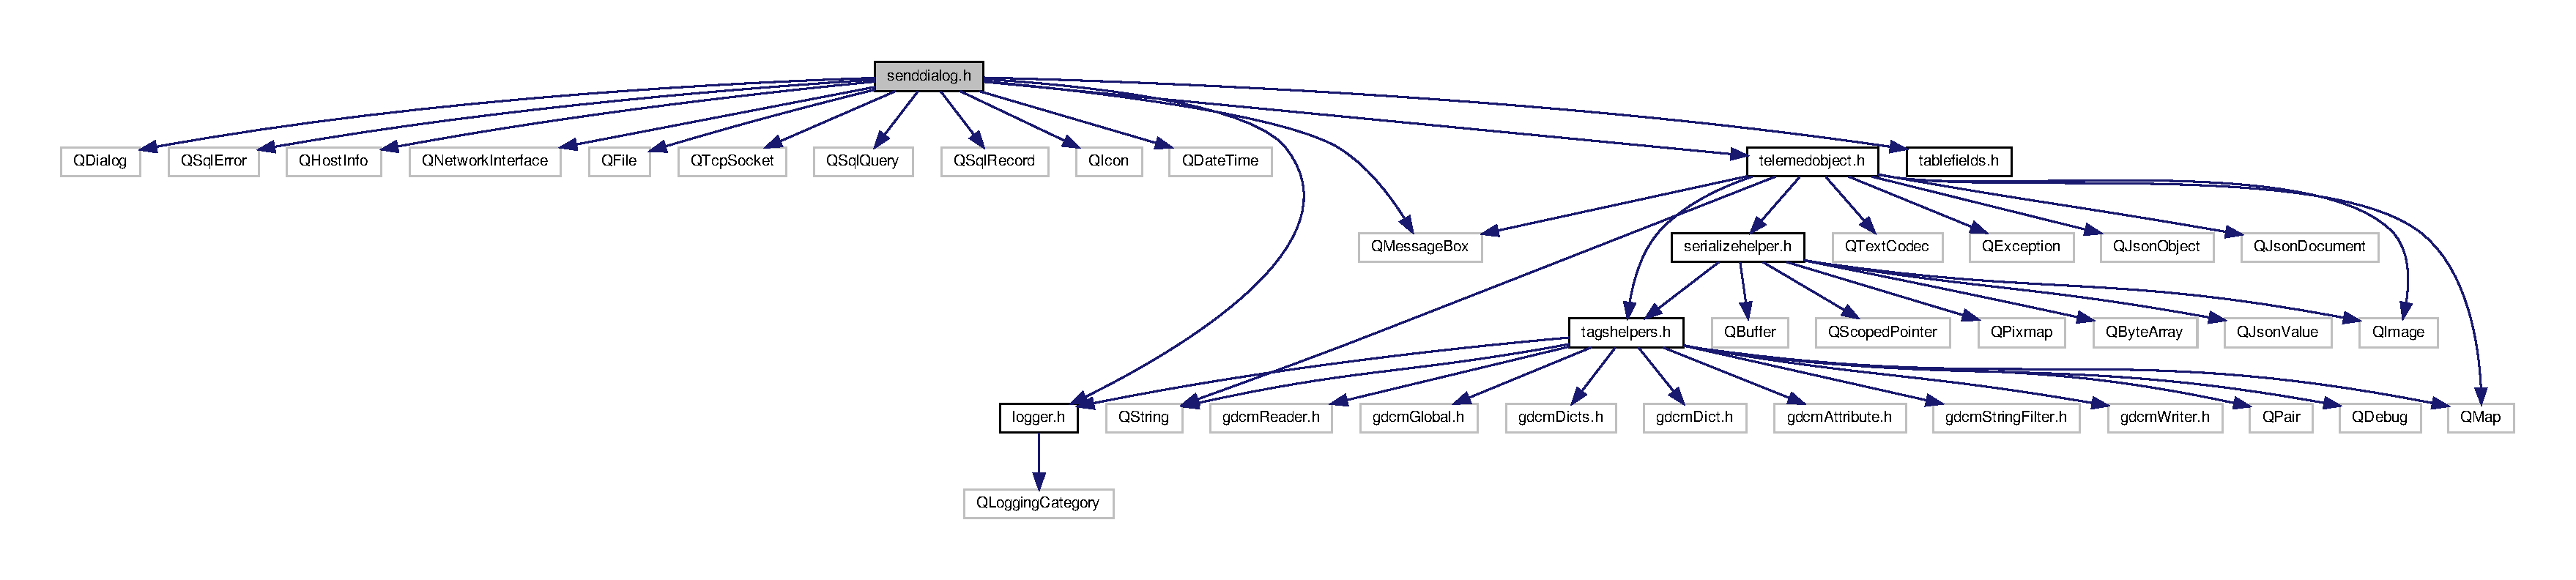
\includegraphics[width=350pt]{senddialog_8h__incl}
\end{center}
\end{figure}
Граф файлов, в которые включается этот файл\+:\nopagebreak
\begin{figure}[H]
\begin{center}
\leavevmode
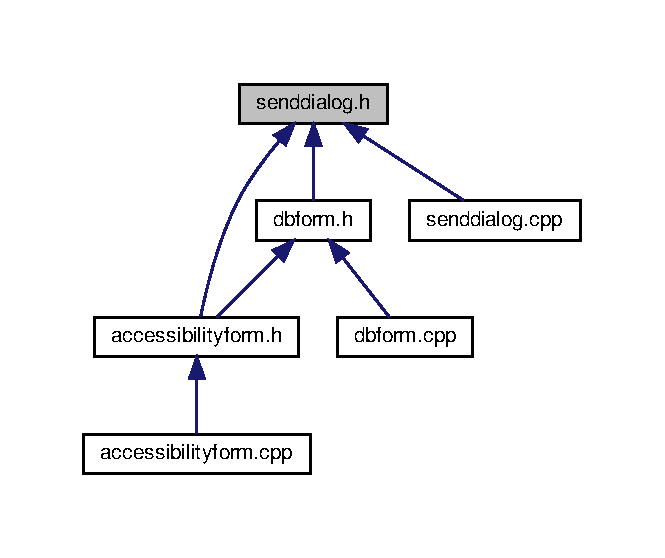
\includegraphics[width=319pt]{senddialog_8h__dep__incl}
\end{center}
\end{figure}
\subsection*{Классы}
\begin{DoxyCompactItemize}
\item 
class \hyperlink{classSendDialog}{Send\+Dialog}
\begin{DoxyCompactList}\small\item\em Класс формы отправки запроса \end{DoxyCompactList}\end{DoxyCompactItemize}
\subsection*{Пространства имен}
\begin{DoxyCompactItemize}
\item 
 \hyperlink{namespaceUi}{Ui}
\end{DoxyCompactItemize}
\subsection*{Определения типов}
\begin{DoxyCompactItemize}
\item 
using \hyperlink{senddialog_8h_aa9b1321518febdee7323e4994ecc1ec3}{id\+With\+Object} = Q\+Pair$<$ \hyperlink{classTeleMedObject}{Tele\+Med\+Object}, int $>$
\end{DoxyCompactItemize}


\subsection{Типы}
\mbox{\Hypertarget{senddialog_8h_aa9b1321518febdee7323e4994ecc1ec3}\label{senddialog_8h_aa9b1321518febdee7323e4994ecc1ec3}} 
\index{senddialog.\+h@{senddialog.\+h}!id\+With\+Object@{id\+With\+Object}}
\index{id\+With\+Object@{id\+With\+Object}!senddialog.\+h@{senddialog.\+h}}
\subsubsection{\texorpdfstring{id\+With\+Object}{idWithObject}}
{\footnotesize\ttfamily using \hyperlink{senddialog_8h_aa9b1321518febdee7323e4994ecc1ec3}{id\+With\+Object} =  Q\+Pair$<$\hyperlink{classTeleMedObject}{Tele\+Med\+Object}, int$>$}


\hypertarget{serializehelper_8cpp}{}\section{Файл serializehelper.\+cpp}
\label{serializehelper_8cpp}\index{serializehelper.\+cpp@{serializehelper.\+cpp}}
{\ttfamily \#include $<$serializehelper.\+h$>$}\newline
Граф включаемых заголовочных файлов для serializehelper.\+cpp\+:\nopagebreak
\begin{figure}[H]
\begin{center}
\leavevmode
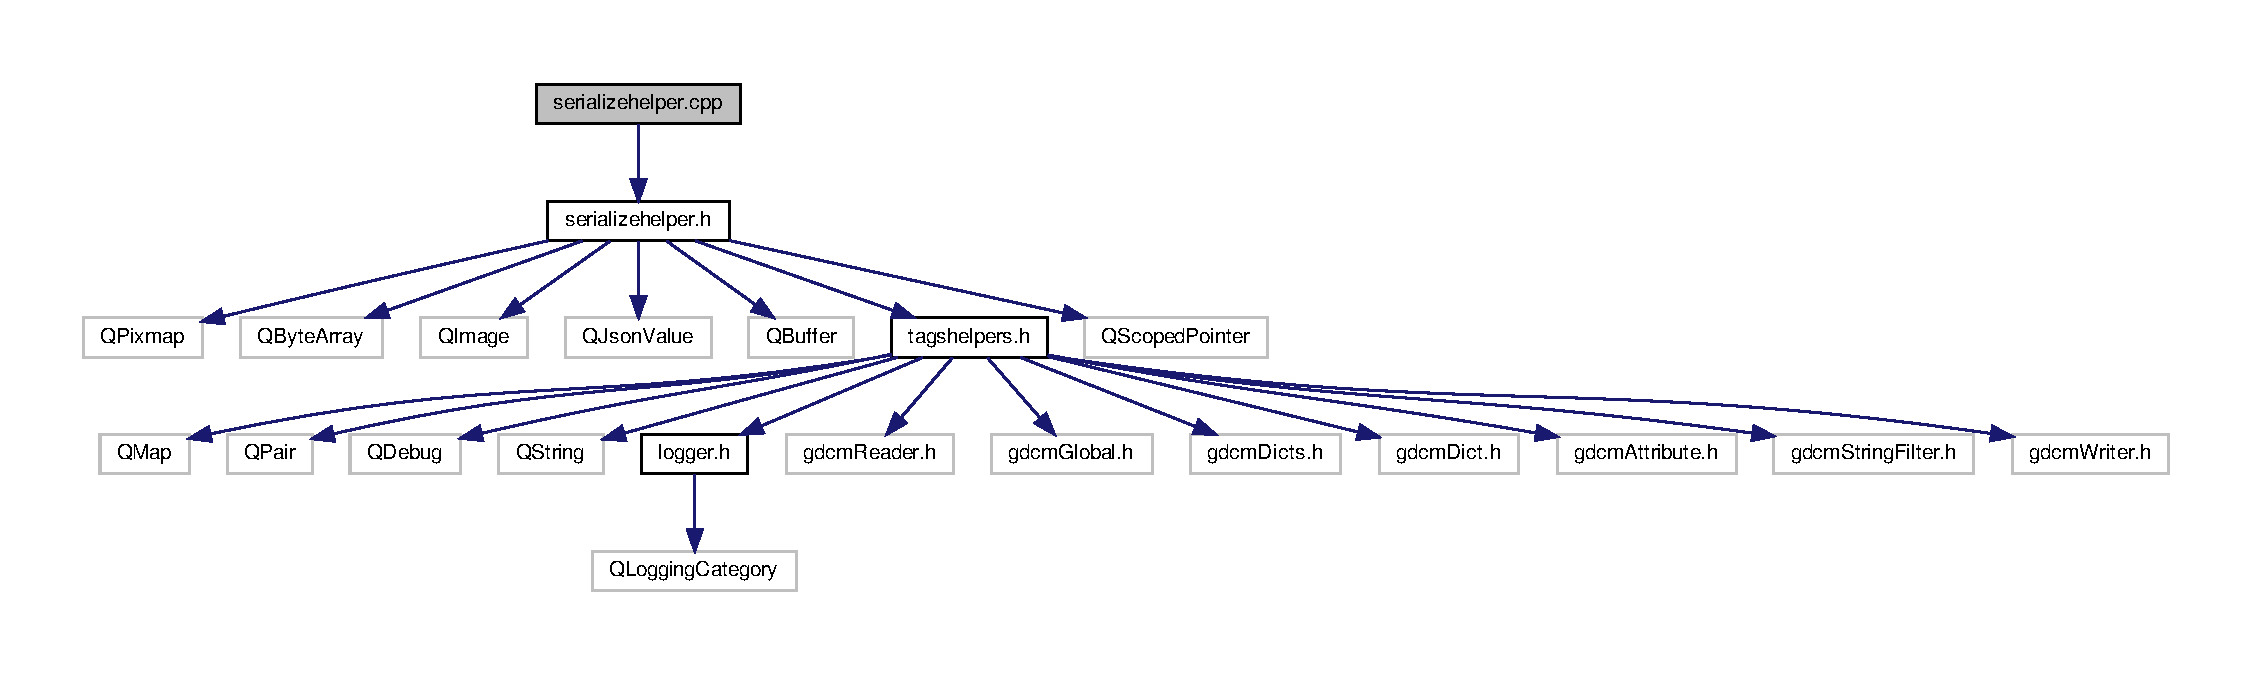
\includegraphics[width=350pt]{serializehelper_8cpp__incl}
\end{center}
\end{figure}
\subsection*{Пространства имен}
\begin{DoxyCompactItemize}
\item 
 \hyperlink{namespaceSerialize}{Serialize}
\end{DoxyCompactItemize}
\subsection*{Функции}
\begin{DoxyCompactItemize}
\item 
Q\+Byte\+Array \hyperlink{namespaceSerialize_a11412877176c667f31a331bfac95d7e1}{Serialize\+::image\+To\+Byte\+Array} (const Q\+Image \&image)
\begin{DoxyCompactList}\small\item\em image\+To\+Byte\+Array \end{DoxyCompactList}\item 
Q\+Image \hyperlink{namespaceSerialize_ad70935346b9a0522990d0ff87e963a26}{Serialize\+::byte\+Array\+To\+Image} (const Q\+Byte\+Array \&ba)
\begin{DoxyCompactList}\small\item\em byte\+Array\+To\+Image \end{DoxyCompactList}\item 
Q\+Json\+Value \hyperlink{namespaceSerialize_a794b837e3f9323b238c5b4d115f5c78b}{Serialize\+::json\+Val\+From\+Image} (const Q\+Image \&p)
\begin{DoxyCompactList}\small\item\em json\+Val\+From\+Image \end{DoxyCompactList}\item 
Q\+Image \hyperlink{namespaceSerialize_a966ed9963741cb19a07f8b057faae920}{Serialize\+::image\+From} (const Q\+Json\+Value \&val)
\begin{DoxyCompactList}\small\item\em image\+From \end{DoxyCompactList}\end{DoxyCompactItemize}

\hypertarget{serializehelper_8h}{}\section{Файл serializehelper.\+h}
\label{serializehelper_8h}\index{serializehelper.\+h@{serializehelper.\+h}}
{\ttfamily \#include $<$Q\+Pixmap$>$}\newline
{\ttfamily \#include $<$Q\+Byte\+Array$>$}\newline
{\ttfamily \#include $<$Q\+Image$>$}\newline
{\ttfamily \#include $<$Q\+Json\+Value$>$}\newline
{\ttfamily \#include $<$Q\+Buffer$>$}\newline
{\ttfamily \#include $<$tagshelpers.\+h$>$}\newline
{\ttfamily \#include $<$Q\+Scoped\+Pointer$>$}\newline
Граф включаемых заголовочных файлов для serializehelper.\+h\+:\nopagebreak
\begin{figure}[H]
\begin{center}
\leavevmode
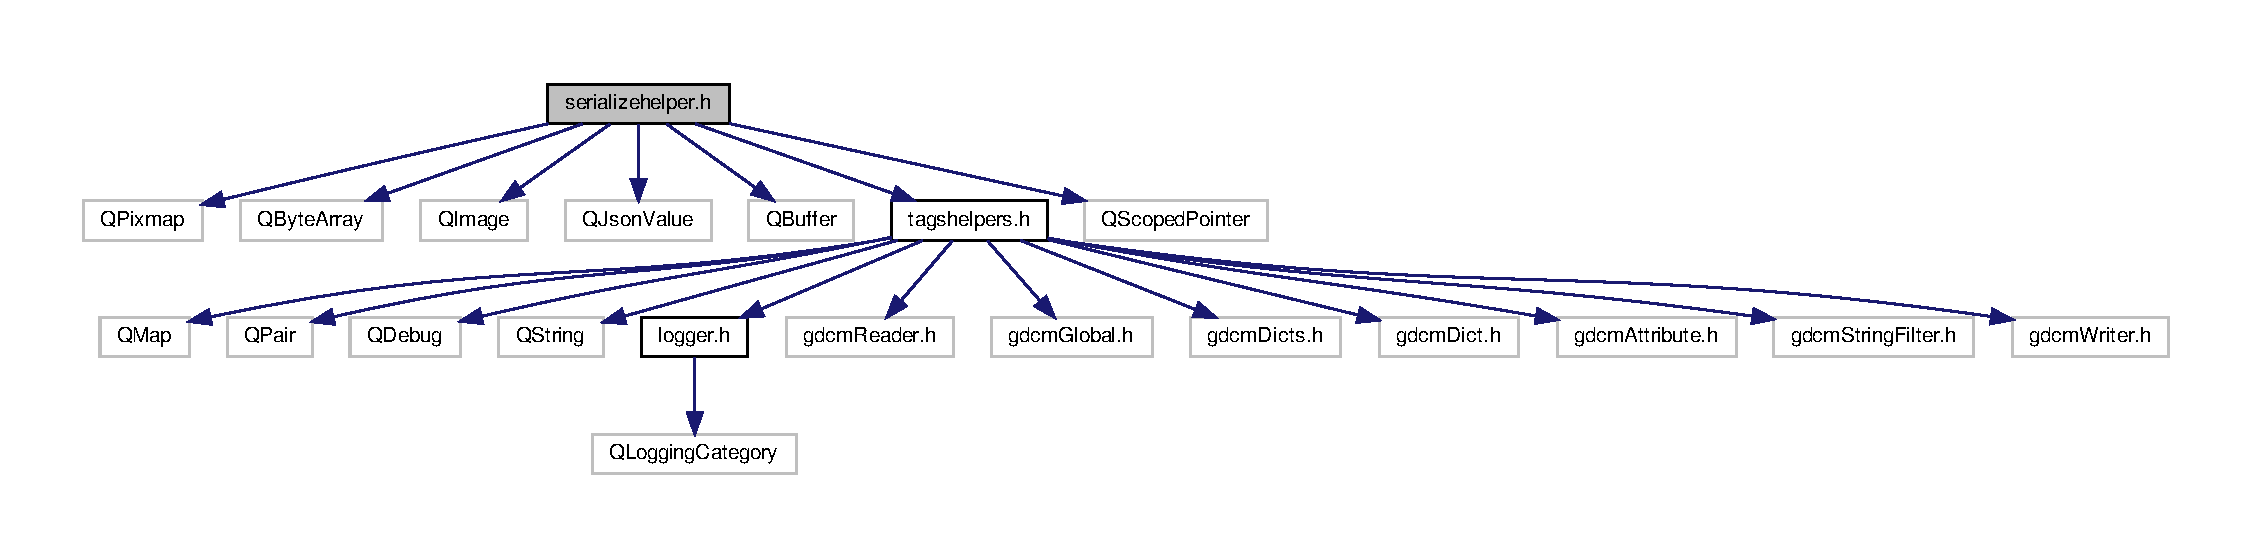
\includegraphics[width=350pt]{serializehelper_8h__incl}
\end{center}
\end{figure}
Граф файлов, в которые включается этот файл\+:\nopagebreak
\begin{figure}[H]
\begin{center}
\leavevmode
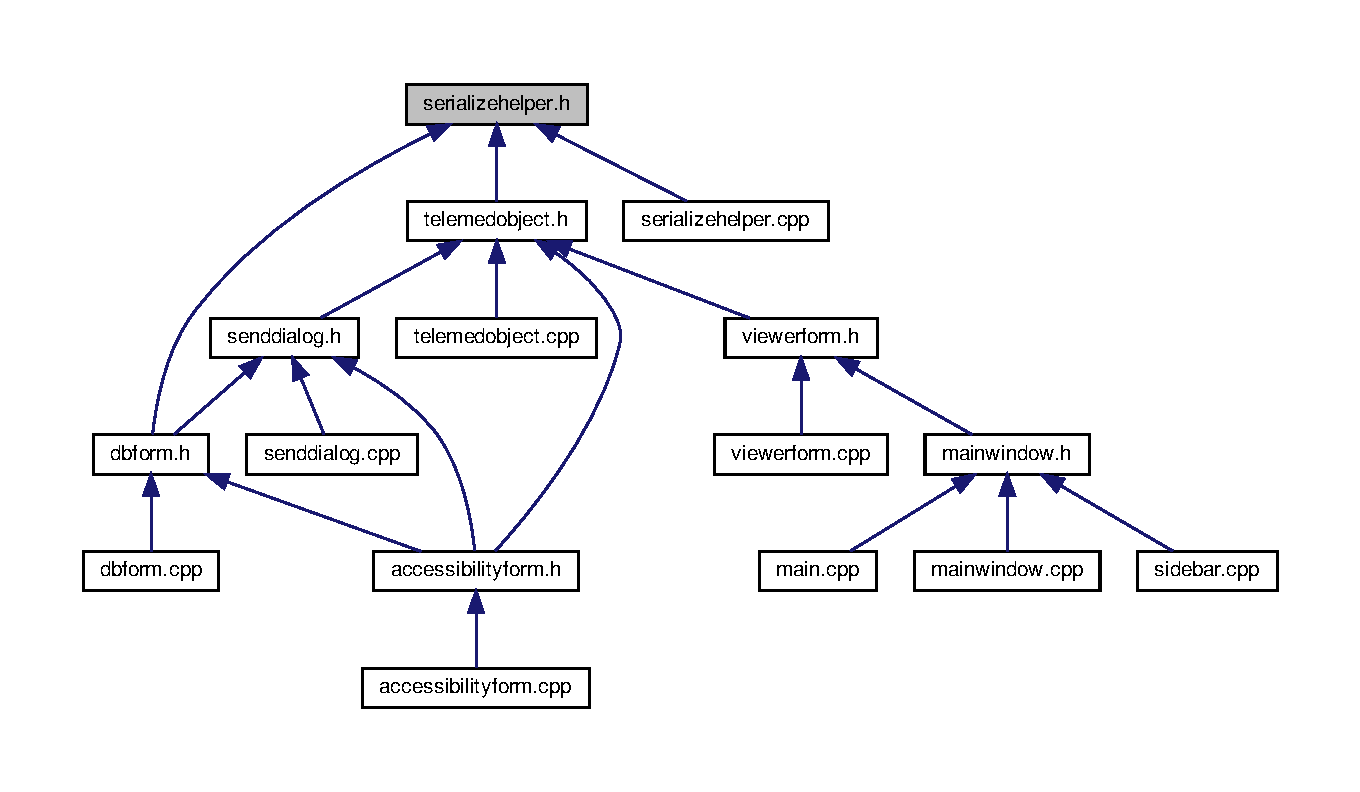
\includegraphics[width=350pt]{serializehelper_8h__dep__incl}
\end{center}
\end{figure}
\subsection*{Пространства имен}
\begin{DoxyCompactItemize}
\item 
 \hyperlink{namespaceSerialize}{Serialize}
\end{DoxyCompactItemize}
\subsection*{Определения типов}
\begin{DoxyCompactItemize}
\item 
using \hyperlink{serializehelper_8h_a8865f4251cec2170c8651965cbb8d5da}{add\+Info\+Map} = Q\+Map$<$ Q\+String, Q\+String $>$
\end{DoxyCompactItemize}
\subsection*{Функции}
\begin{DoxyCompactItemize}
\item 
Q\+Byte\+Array \hyperlink{namespaceSerialize_a11412877176c667f31a331bfac95d7e1}{Serialize\+::image\+To\+Byte\+Array} (const Q\+Image \&image)
\begin{DoxyCompactList}\small\item\em image\+To\+Byte\+Array \end{DoxyCompactList}\item 
Q\+Image \hyperlink{namespaceSerialize_ad70935346b9a0522990d0ff87e963a26}{Serialize\+::byte\+Array\+To\+Image} (const Q\+Byte\+Array \&ba)
\begin{DoxyCompactList}\small\item\em byte\+Array\+To\+Image \end{DoxyCompactList}\item 
Q\+Json\+Value \hyperlink{namespaceSerialize_a794b837e3f9323b238c5b4d115f5c78b}{Serialize\+::json\+Val\+From\+Image} (const Q\+Image \&p)
\begin{DoxyCompactList}\small\item\em json\+Val\+From\+Image \end{DoxyCompactList}\item 
Q\+Image \hyperlink{namespaceSerialize_a966ed9963741cb19a07f8b057faae920}{Serialize\+::image\+From} (const Q\+Json\+Value \&val)
\begin{DoxyCompactList}\small\item\em image\+From \end{DoxyCompactList}\item 
{\footnotesize template$<$class T $>$ }\\auto \hyperlink{namespaceSerialize_a5318048e43f2cacc610f177d093283f8}{Serialize\+::dict\+To\+Byte\+Array} (const T \&dict) -\/$>$ Q\+Byte\+Array
\begin{DoxyCompactList}\small\item\em dict\+To\+Byte\+Array \end{DoxyCompactList}\item 
{\footnotesize template$<$class T $>$ }\\T \hyperlink{namespaceSerialize_aac818c4b807e223e916bbe829e0d86ea}{Serialize\+::byte\+Array\+To\+Dict} (Q\+Byte\+Array $\ast$ba)
\begin{DoxyCompactList}\small\item\em byte\+Array\+To\+Dict \end{DoxyCompactList}\item 
{\footnotesize template$<$class T $>$ }\\T \hyperlink{namespaceSerialize_ac2bf64c91d863df6a6c6149c7a482af0}{Serialize\+::dict\+From\+Base64} (const Q\+Json\+Value \&value)
\begin{DoxyCompactList}\small\item\em dict\+From\+Base64 \end{DoxyCompactList}\end{DoxyCompactItemize}


\subsection{Типы}
\mbox{\Hypertarget{serializehelper_8h_a8865f4251cec2170c8651965cbb8d5da}\label{serializehelper_8h_a8865f4251cec2170c8651965cbb8d5da}} 
\index{serializehelper.\+h@{serializehelper.\+h}!add\+Info\+Map@{add\+Info\+Map}}
\index{add\+Info\+Map@{add\+Info\+Map}!serializehelper.\+h@{serializehelper.\+h}}
\subsubsection{\texorpdfstring{add\+Info\+Map}{addInfoMap}}
{\footnotesize\ttfamily using \hyperlink{dbform_8h_a1ec1a645f41e1c6544d384ca863a936c}{add\+Info\+Map} =  Q\+Map$<$Q\+String, Q\+String$>$}


\hypertarget{server_8cpp}{}\section{Файл server.\+cpp}
\label{server_8cpp}\index{server.\+cpp@{server.\+cpp}}
{\ttfamily \#include \char`\"{}server.\+h\char`\"{}}\newline
Граф включаемых заголовочных файлов для server.\+cpp\+:\nopagebreak
\begin{figure}[H]
\begin{center}
\leavevmode
\includegraphics[width=350pt]{server_8cpp__incl}
\end{center}
\end{figure}

\hypertarget{server_8h}{}\section{Файл server.\+h}
\label{server_8h}\index{server.\+h@{server.\+h}}
{\ttfamily \#include $<$Q\+Tcp\+Server$>$}\newline
{\ttfamily \#include $<$Q\+Tcp\+Socket$>$}\newline
{\ttfamily \#include $<$Q\+Abstract\+Socket$>$}\newline
{\ttfamily \#include $<$logger.\+h$>$}\newline
{\ttfamily \#include $<$client.\+h$>$}\newline
Граф включаемых заголовочных файлов для server.\+h\+:\nopagebreak
\begin{figure}[H]
\begin{center}
\leavevmode
\includegraphics[width=350pt]{server_8h__incl}
\end{center}
\end{figure}
Граф файлов, в которые включается этот файл\+:\nopagebreak
\begin{figure}[H]
\begin{center}
\leavevmode
\includegraphics[width=338pt]{server_8h__dep__incl}
\end{center}
\end{figure}
\subsection*{Классы}
\begin{DoxyCompactItemize}
\item 
class \hyperlink{classServer}{Server}
\begin{DoxyCompactList}\small\item\em Класс сервера \end{DoxyCompactList}\end{DoxyCompactItemize}

\hypertarget{sidebar_8cpp}{}\section{Файл sidebar.\+cpp}
\label{sidebar_8cpp}\index{sidebar.\+cpp@{sidebar.\+cpp}}
{\ttfamily \#include \char`\"{}sidebar.\+h\char`\"{}}\newline
{\ttfamily \#include \char`\"{}mainwindow.\+h\char`\"{}}\newline
{\ttfamily \#include $<$Q\+Paint\+Event$>$}\newline
{\ttfamily \#include $<$Q\+Painter$>$}\newline
{\ttfamily \#include $<$Q\+Debug$>$}\newline
{\ttfamily \#include $<$Q\+Event$>$}\newline
Граф включаемых заголовочных файлов для sidebar.\+cpp\+:\nopagebreak
\begin{figure}[H]
\begin{center}
\leavevmode
\includegraphics[width=350pt]{sidebar_8cpp__incl}
\end{center}
\end{figure}
\subsection*{Макросы}
\begin{DoxyCompactItemize}
\item 
\#define \hyperlink{sidebar_8cpp_a2d683d41cc5769ee8dbfe04549536f2e}{action\+\_\+height}~120
\end{DoxyCompactItemize}


\subsection{Макросы}
\mbox{\Hypertarget{sidebar_8cpp_a2d683d41cc5769ee8dbfe04549536f2e}\label{sidebar_8cpp_a2d683d41cc5769ee8dbfe04549536f2e}} 
\index{sidebar.\+cpp@{sidebar.\+cpp}!action\+\_\+height@{action\+\_\+height}}
\index{action\+\_\+height@{action\+\_\+height}!sidebar.\+cpp@{sidebar.\+cpp}}
\subsubsection{\texorpdfstring{action\+\_\+height}{action\_height}}
{\footnotesize\ttfamily \#define action\+\_\+height~120}


\hypertarget{sidebar_8h}{}\section{Файл sidebar.\+h}
\label{sidebar_8h}\index{sidebar.\+h@{sidebar.\+h}}
{\ttfamily \#include $<$Q\+Action$>$}\newline
{\ttfamily \#include $<$Q\+Widget$>$}\newline
{\ttfamily \#include $<$logger.\+h$>$}\newline
Граф включаемых заголовочных файлов для sidebar.\+h\+:\nopagebreak
\begin{figure}[H]
\begin{center}
\leavevmode
\includegraphics[width=298pt]{sidebar_8h__incl}
\end{center}
\end{figure}
Граф файлов, в которые включается этот файл\+:\nopagebreak
\begin{figure}[H]
\begin{center}
\leavevmode
\includegraphics[width=147pt]{sidebar_8h__dep__incl}
\end{center}
\end{figure}
\subsection*{Классы}
\begin{DoxyCompactItemize}
\item 
class \hyperlink{classSideBar}{Side\+Bar}
\begin{DoxyCompactList}\small\item\em Класс формы боковой панели выбора виджета \end{DoxyCompactList}\end{DoxyCompactItemize}

\hypertarget{tablefields_8h}{}\section{Файл tablefields.\+h}
\label{tablefields_8h}\index{tablefields.\+h@{tablefields.\+h}}
Граф файлов, в которые включается этот файл\+:\nopagebreak
\begin{figure}[H]
\begin{center}
\leavevmode
\includegraphics[width=319pt]{tablefields_8h__dep__incl}
\end{center}
\end{figure}
\subsection*{Пространства имен}
\begin{DoxyCompactItemize}
\item 
 \hyperlink{namespacetableFields}{table\+Fields}
\end{DoxyCompactItemize}
\subsection*{Перечисления}
\begin{DoxyCompactItemize}
\item 
enum \hyperlink{namespacetableFields_af3f3b90a55c2fc0e89652786698aff33}{table\+Fields\+::table\+Fields} \{ \newline
\hyperlink{namespacetableFields_af3f3b90a55c2fc0e89652786698aff33a3688697bcb72b96772a0b8bba66cf1f7}{table\+Fields\+::table\+\_\+id} = 0, 
\hyperlink{namespacetableFields_af3f3b90a55c2fc0e89652786698aff33aac6d4c2d5e73ed2e112948441fa690f2}{table\+Fields\+::table\+\_\+name} = 1, 
\hyperlink{namespacetableFields_af3f3b90a55c2fc0e89652786698aff33a0fbe15558786dbadd11790fa61e16cda}{table\+Fields\+::table\+\_\+image} = 2, 
\hyperlink{namespacetableFields_af3f3b90a55c2fc0e89652786698aff33a4699aeeba4e2c1b5addebc6fde4e004e}{table\+Fields\+::table\+\_\+data} = 3, 
\newline
\hyperlink{namespacetableFields_af3f3b90a55c2fc0e89652786698aff33a69b6cda96cbc1bd9d9fed0c8a0446d14}{table\+Fields\+::table\+\_\+request} = 4, 
\hyperlink{namespacetableFields_af3f3b90a55c2fc0e89652786698aff33a7d5985177bdc214aa76c2956da19b292}{table\+Fields\+::table\+\_\+response} = 5, 
\hyperlink{namespacetableFields_af3f3b90a55c2fc0e89652786698aff33a2488fe0a3fd10b94548a37839474f12a}{table\+Fields\+::table\+\_\+request\+\_\+date} = 6, 
\hyperlink{namespacetableFields_af3f3b90a55c2fc0e89652786698aff33a08521c2e57d6cd782177ff9410c234a7}{table\+Fields\+::table\+\_\+response\+\_\+date} = 7, 
\newline
\hyperlink{namespacetableFields_af3f3b90a55c2fc0e89652786698aff33af6c67a88169df220165a3f4b3edc5ca7}{table\+Fields\+::table\+\_\+requester} = 8, 
\hyperlink{namespacetableFields_af3f3b90a55c2fc0e89652786698aff33abd83777ee433cf1acf2c16b45f03e677}{table\+Fields\+::table\+\_\+responser} = 9
 \}
\end{DoxyCompactItemize}

\hypertarget{tagshelpers_8cpp}{}\section{Файл tagshelpers.\+cpp}
\label{tagshelpers_8cpp}\index{tagshelpers.\+cpp@{tagshelpers.\+cpp}}
{\ttfamily \#include $<$tagshelpers.\+h$>$}\newline
Граф включаемых заголовочных файлов для tagshelpers.\+cpp\+:\nopagebreak
\begin{figure}[H]
\begin{center}
\leavevmode
\includegraphics[width=350pt]{tagshelpers_8cpp__incl}
\end{center}
\end{figure}
\subsection*{Функции}
\begin{DoxyCompactItemize}
\item 
\hyperlink{tagshelpers_8h_ae25d30658f61420b88a380dc9e40bb74}{dicom\+Dict} \hyperlink{tagshelpers_8cpp_a5de97453445a235f3447e900ec778ee4}{get\+Tags} (const char $\ast$filename)
\begin{DoxyCompactList}\small\item\em get\+Tags \end{DoxyCompactList}\item 
bool \hyperlink{tagshelpers_8cpp_a597aa9a6202848f5e5a44d57c281908e}{set\+Tag} (const std\+::string \&offset, const std\+::string \&value, const char $\ast$filename)
\begin{DoxyCompactList}\small\item\em set\+Tag \end{DoxyCompactList}\item 
Q\+String \hyperlink{tagshelpers_8cpp_a34c2e8ab74c0f6438a86a1c281ef15a6}{get\+Name\+From\+Dict} (\hyperlink{tagshelpers_8h_ae25d30658f61420b88a380dc9e40bb74}{dicom\+Dict} \&dict)
\begin{DoxyCompactList}\small\item\em get\+Name\+From\+Dict \end{DoxyCompactList}\end{DoxyCompactItemize}


\subsection{Функции}
\mbox{\Hypertarget{tagshelpers_8cpp_a34c2e8ab74c0f6438a86a1c281ef15a6}\label{tagshelpers_8cpp_a34c2e8ab74c0f6438a86a1c281ef15a6}} 
\index{tagshelpers.\+cpp@{tagshelpers.\+cpp}!get\+Name\+From\+Dict@{get\+Name\+From\+Dict}}
\index{get\+Name\+From\+Dict@{get\+Name\+From\+Dict}!tagshelpers.\+cpp@{tagshelpers.\+cpp}}
\subsubsection{\texorpdfstring{get\+Name\+From\+Dict()}{getNameFromDict()}}
{\footnotesize\ttfamily Q\+String get\+Name\+From\+Dict (\begin{DoxyParamCaption}\item[{\hyperlink{tagshelpers_8h_ae25d30658f61420b88a380dc9e40bb74}{dicom\+Dict} \&}]{dict }\end{DoxyParamCaption})}



get\+Name\+From\+Dict 


\begin{DoxyParams}{Аргументы}
{\em dict} & Словарь с данными об исследовании \\
\hline
\end{DoxyParams}
\begin{DoxyReturn}{Возвращает}
Имя пациента
\end{DoxyReturn}
Функция получает имя пациента из набора данных об исследовании \mbox{\Hypertarget{tagshelpers_8cpp_a5de97453445a235f3447e900ec778ee4}\label{tagshelpers_8cpp_a5de97453445a235f3447e900ec778ee4}} 
\index{tagshelpers.\+cpp@{tagshelpers.\+cpp}!get\+Tags@{get\+Tags}}
\index{get\+Tags@{get\+Tags}!tagshelpers.\+cpp@{tagshelpers.\+cpp}}
\subsubsection{\texorpdfstring{get\+Tags()}{getTags()}}
{\footnotesize\ttfamily \hyperlink{tagshelpers_8h_ae25d30658f61420b88a380dc9e40bb74}{dicom\+Dict} get\+Tags (\begin{DoxyParamCaption}\item[{const char $\ast$}]{filename }\end{DoxyParamCaption})}



get\+Tags 


\begin{DoxyParams}{Аргументы}
{\em filename} & Имя файла типа dcm \\
\hline
\end{DoxyParams}
\begin{DoxyReturn}{Возвращает}
Словарь с данными из файла в формате dicom
\end{DoxyReturn}
Функция для получения тегов dicom из файла типа dcm в словарь \mbox{\Hypertarget{tagshelpers_8cpp_a597aa9a6202848f5e5a44d57c281908e}\label{tagshelpers_8cpp_a597aa9a6202848f5e5a44d57c281908e}} 
\index{tagshelpers.\+cpp@{tagshelpers.\+cpp}!set\+Tag@{set\+Tag}}
\index{set\+Tag@{set\+Tag}!tagshelpers.\+cpp@{tagshelpers.\+cpp}}
\subsubsection{\texorpdfstring{set\+Tag()}{setTag()}}
{\footnotesize\ttfamily bool set\+Tag (\begin{DoxyParamCaption}\item[{const std\+::string \&}]{offset,  }\item[{const std\+::string \&}]{value,  }\item[{const char $\ast$}]{filename }\end{DoxyParamCaption})}



set\+Tag 


\begin{DoxyParams}{Аргументы}
{\em offset} & Сдвиг по файлу, на котором находится искомый тег \\
\hline
{\em value} & Значение тега для записи \\
\hline
{\em filename} & Имя файла на файловой системе \\
\hline
\end{DoxyParams}
\begin{DoxyReturn}{Возвращает}
true -\/ если запись была успешна
\end{DoxyReturn}
Функция для записи собственного значения в существующий тег файла dcm 
\hypertarget{tagshelpers_8h}{}\section{Файл tagshelpers.\+h}
\label{tagshelpers_8h}\index{tagshelpers.\+h@{tagshelpers.\+h}}
{\ttfamily \#include $<$Q\+Map$>$}\newline
{\ttfamily \#include $<$Q\+Pair$>$}\newline
{\ttfamily \#include $<$Q\+Debug$>$}\newline
{\ttfamily \#include $<$Q\+String$>$}\newline
{\ttfamily \#include $<$logger.\+h$>$}\newline
{\ttfamily \#include \char`\"{}gdcm\+Reader.\+h\char`\"{}}\newline
{\ttfamily \#include \char`\"{}gdcm\+Global.\+h\char`\"{}}\newline
{\ttfamily \#include \char`\"{}gdcm\+Dicts.\+h\char`\"{}}\newline
{\ttfamily \#include \char`\"{}gdcm\+Dict.\+h\char`\"{}}\newline
{\ttfamily \#include \char`\"{}gdcm\+Attribute.\+h\char`\"{}}\newline
{\ttfamily \#include \char`\"{}gdcm\+String\+Filter.\+h\char`\"{}}\newline
{\ttfamily \#include \char`\"{}gdcm\+Writer.\+h\char`\"{}}\newline
Граф включаемых заголовочных файлов для tagshelpers.\+h\+:\nopagebreak
\begin{figure}[H]
\begin{center}
\leavevmode
\includegraphics[width=350pt]{tagshelpers_8h__incl}
\end{center}
\end{figure}
Граф файлов, в которые включается этот файл\+:\nopagebreak
\begin{figure}[H]
\begin{center}
\leavevmode
\includegraphics[width=350pt]{tagshelpers_8h__dep__incl}
\end{center}
\end{figure}
\subsection*{Определения типов}
\begin{DoxyCompactItemize}
\item 
using \hyperlink{tagshelpers_8h_ae25d30658f61420b88a380dc9e40bb74}{dicom\+Dict} = Q\+Map$<$ Q\+String, Q\+Pair$<$ Q\+String, Q\+String $>$ $>$
\end{DoxyCompactItemize}
\subsection*{Функции}
\begin{DoxyCompactItemize}
\item 
\hyperlink{tagshelpers_8h_ae25d30658f61420b88a380dc9e40bb74}{dicom\+Dict} \hyperlink{tagshelpers_8h_a5de97453445a235f3447e900ec778ee4}{get\+Tags} (const char $\ast$filename)
\begin{DoxyCompactList}\small\item\em get\+Tags \end{DoxyCompactList}\item 
bool \hyperlink{tagshelpers_8h_a597aa9a6202848f5e5a44d57c281908e}{set\+Tag} (const std\+::string \&offset, const std\+::string \&value, const char $\ast$filename)
\begin{DoxyCompactList}\small\item\em set\+Tag \end{DoxyCompactList}\item 
Q\+String \hyperlink{tagshelpers_8h_a34c2e8ab74c0f6438a86a1c281ef15a6}{get\+Name\+From\+Dict} (\hyperlink{tagshelpers_8h_ae25d30658f61420b88a380dc9e40bb74}{dicom\+Dict} \&dict)
\begin{DoxyCompactList}\small\item\em get\+Name\+From\+Dict \end{DoxyCompactList}\end{DoxyCompactItemize}
\subsection*{Переменные}
\begin{DoxyCompactItemize}
\item 
static \hyperlink{tagshelpers_8h_ae25d30658f61420b88a380dc9e40bb74}{dicom\+Dict} \hyperlink{tagshelpers_8h_a244b7433b44125ac2757c8be01eaec41}{Tags\+Map}
\end{DoxyCompactItemize}


\subsection{Типы}
\mbox{\Hypertarget{tagshelpers_8h_ae25d30658f61420b88a380dc9e40bb74}\label{tagshelpers_8h_ae25d30658f61420b88a380dc9e40bb74}} 
\index{tagshelpers.\+h@{tagshelpers.\+h}!dicom\+Dict@{dicom\+Dict}}
\index{dicom\+Dict@{dicom\+Dict}!tagshelpers.\+h@{tagshelpers.\+h}}
\subsubsection{\texorpdfstring{dicom\+Dict}{dicomDict}}
{\footnotesize\ttfamily using \hyperlink{tagshelpers_8h_ae25d30658f61420b88a380dc9e40bb74}{dicom\+Dict} =  Q\+Map$<$Q\+String, Q\+Pair$<$Q\+String, Q\+String$>$ $>$}



\subsection{Функции}
\mbox{\Hypertarget{tagshelpers_8h_a34c2e8ab74c0f6438a86a1c281ef15a6}\label{tagshelpers_8h_a34c2e8ab74c0f6438a86a1c281ef15a6}} 
\index{tagshelpers.\+h@{tagshelpers.\+h}!get\+Name\+From\+Dict@{get\+Name\+From\+Dict}}
\index{get\+Name\+From\+Dict@{get\+Name\+From\+Dict}!tagshelpers.\+h@{tagshelpers.\+h}}
\subsubsection{\texorpdfstring{get\+Name\+From\+Dict()}{getNameFromDict()}}
{\footnotesize\ttfamily Q\+String get\+Name\+From\+Dict (\begin{DoxyParamCaption}\item[{\hyperlink{tagshelpers_8h_ae25d30658f61420b88a380dc9e40bb74}{dicom\+Dict} \&}]{dict }\end{DoxyParamCaption})}



get\+Name\+From\+Dict 


\begin{DoxyParams}{Аргументы}
{\em dict} & Словарь с данными об исследовании \\
\hline
\end{DoxyParams}
\begin{DoxyReturn}{Возвращает}
Имя пациента
\end{DoxyReturn}
Функция получает имя пациента из набора данных об исследовании \mbox{\Hypertarget{tagshelpers_8h_a5de97453445a235f3447e900ec778ee4}\label{tagshelpers_8h_a5de97453445a235f3447e900ec778ee4}} 
\index{tagshelpers.\+h@{tagshelpers.\+h}!get\+Tags@{get\+Tags}}
\index{get\+Tags@{get\+Tags}!tagshelpers.\+h@{tagshelpers.\+h}}
\subsubsection{\texorpdfstring{get\+Tags()}{getTags()}}
{\footnotesize\ttfamily \hyperlink{tagshelpers_8h_ae25d30658f61420b88a380dc9e40bb74}{dicom\+Dict} get\+Tags (\begin{DoxyParamCaption}\item[{const char $\ast$}]{filename }\end{DoxyParamCaption})}



get\+Tags 


\begin{DoxyParams}{Аргументы}
{\em filename} & Имя файла типа dcm \\
\hline
\end{DoxyParams}
\begin{DoxyReturn}{Возвращает}
Словарь с данными из файла в формате dicom
\end{DoxyReturn}
Функция для получения тегов dicom из файла типа dcm в словарь \mbox{\Hypertarget{tagshelpers_8h_a597aa9a6202848f5e5a44d57c281908e}\label{tagshelpers_8h_a597aa9a6202848f5e5a44d57c281908e}} 
\index{tagshelpers.\+h@{tagshelpers.\+h}!set\+Tag@{set\+Tag}}
\index{set\+Tag@{set\+Tag}!tagshelpers.\+h@{tagshelpers.\+h}}
\subsubsection{\texorpdfstring{set\+Tag()}{setTag()}}
{\footnotesize\ttfamily bool set\+Tag (\begin{DoxyParamCaption}\item[{const std\+::string \&}]{offset,  }\item[{const std\+::string \&}]{value,  }\item[{const char $\ast$}]{filename }\end{DoxyParamCaption})}



set\+Tag 


\begin{DoxyParams}{Аргументы}
{\em offset} & Сдвиг по файлу, на котором находится искомый тег \\
\hline
{\em value} & Значение тега для записи \\
\hline
{\em filename} & Имя файла на файловой системе \\
\hline
\end{DoxyParams}
\begin{DoxyReturn}{Возвращает}
true -\/ если запись была успешна
\end{DoxyReturn}
Функция для записи собственного значения в существующий тег файла dcm 

\subsection{Переменные}
\mbox{\Hypertarget{tagshelpers_8h_a244b7433b44125ac2757c8be01eaec41}\label{tagshelpers_8h_a244b7433b44125ac2757c8be01eaec41}} 
\index{tagshelpers.\+h@{tagshelpers.\+h}!Tags\+Map@{Tags\+Map}}
\index{Tags\+Map@{Tags\+Map}!tagshelpers.\+h@{tagshelpers.\+h}}
\subsubsection{\texorpdfstring{Tags\+Map}{TagsMap}}
{\footnotesize\ttfamily \hyperlink{tagshelpers_8h_ae25d30658f61420b88a380dc9e40bb74}{dicom\+Dict} Tags\+Map\hspace{0.3cm}{\ttfamily [static]}}


\hypertarget{task_8cpp}{}\section{Файл task.\+cpp}
\label{task_8cpp}\index{task.\+cpp@{task.\+cpp}}
{\ttfamily \#include \char`\"{}task.\+h\char`\"{}}\newline
Граф включаемых заголовочных файлов для task.\+cpp\+:\nopagebreak
\begin{figure}[H]
\begin{center}
\leavevmode
\includegraphics[width=350pt]{task_8cpp__incl}
\end{center}
\end{figure}

\hypertarget{task_8h}{}\section{Файл task.\+h}
\label{task_8h}\index{task.\+h@{task.\+h}}
{\ttfamily \#include $<$Q\+Runnable$>$}\newline
{\ttfamily \#include $<$Q\+Byte\+Array$>$}\newline
{\ttfamily \#include $<$Q\+Object$>$}\newline
{\ttfamily \#include $<$logger.\+h$>$}\newline
Граф включаемых заголовочных файлов для task.\+h\+:\nopagebreak
\begin{figure}[H]
\begin{center}
\leavevmode
\includegraphics[width=350pt]{task_8h__incl}
\end{center}
\end{figure}
Граф файлов, в которые включается этот файл\+:\nopagebreak
\begin{figure}[H]
\begin{center}
\leavevmode
\includegraphics[width=350pt]{task_8h__dep__incl}
\end{center}
\end{figure}
\subsection*{Классы}
\begin{DoxyCompactItemize}
\item 
class \hyperlink{classTask}{Task}
\begin{DoxyCompactList}\small\item\em Класс задачи \end{DoxyCompactList}\end{DoxyCompactItemize}

\hypertarget{telemedobject_8cpp}{}\section{Файл telemedobject.\+cpp}
\label{telemedobject_8cpp}\index{telemedobject.\+cpp@{telemedobject.\+cpp}}
{\ttfamily \#include \char`\"{}telemedobject.\+h\char`\"{}}\newline
Граф включаемых заголовочных файлов для telemedobject.\+cpp\+:\nopagebreak
\begin{figure}[H]
\begin{center}
\leavevmode
\includegraphics[width=350pt]{telemedobject_8cpp__incl}
\end{center}
\end{figure}

\hypertarget{telemedobject_8h}{}\section{Файл telemedobject.\+h}
\label{telemedobject_8h}\index{telemedobject.\+h@{telemedobject.\+h}}
{\ttfamily \#include $<$Q\+Image$>$}\newline
{\ttfamily \#include $<$Q\+Map$>$}\newline
{\ttfamily \#include $<$Q\+Text\+Codec$>$}\newline
{\ttfamily \#include $<$Q\+Message\+Box$>$}\newline
{\ttfamily \#include \char`\"{}tagshelpers.\+h\char`\"{}}\newline
{\ttfamily \#include $<$Q\+String$>$}\newline
{\ttfamily \#include $<$Q\+Exception$>$}\newline
{\ttfamily \#include $<$Q\+Json\+Object$>$}\newline
{\ttfamily \#include $<$Q\+Json\+Document$>$}\newline
{\ttfamily \#include \char`\"{}serializehelper.\+h\char`\"{}}\newline
Граф включаемых заголовочных файлов для telemedobject.\+h\+:\nopagebreak
\begin{figure}[H]
\begin{center}
\leavevmode
\includegraphics[width=350pt]{telemedobject_8h__incl}
\end{center}
\end{figure}
Граф файлов, в которые включается этот файл\+:\nopagebreak
\begin{figure}[H]
\begin{center}
\leavevmode
\includegraphics[width=350pt]{telemedobject_8h__dep__incl}
\end{center}
\end{figure}
\subsection*{Классы}
\begin{DoxyCompactItemize}
\item 
class \hyperlink{classTeleMedObjException}{Tele\+Med\+Obj\+Exception}
\begin{DoxyCompactList}\small\item\em Класс исключения при построении объекта информации \end{DoxyCompactList}\item 
class \hyperlink{classTeleMedObject}{Tele\+Med\+Object}
\begin{DoxyCompactList}\small\item\em Класс объекта информации в телемедицинском сеансе \end{DoxyCompactList}\end{DoxyCompactItemize}
\subsection*{Определения типов}
\begin{DoxyCompactItemize}
\item 
using \hyperlink{telemedobject_8h_a8865f4251cec2170c8651965cbb8d5da}{add\+Info\+Map} = Q\+Map$<$ Q\+String, Q\+String $>$
\end{DoxyCompactItemize}


\subsection{Типы}
\mbox{\Hypertarget{telemedobject_8h_a8865f4251cec2170c8651965cbb8d5da}\label{telemedobject_8h_a8865f4251cec2170c8651965cbb8d5da}} 
\index{telemedobject.\+h@{telemedobject.\+h}!add\+Info\+Map@{add\+Info\+Map}}
\index{add\+Info\+Map@{add\+Info\+Map}!telemedobject.\+h@{telemedobject.\+h}}
\subsubsection{\texorpdfstring{add\+Info\+Map}{addInfoMap}}
{\footnotesize\ttfamily using \hyperlink{dbform_8h_a1ec1a645f41e1c6544d384ca863a936c}{add\+Info\+Map} =  Q\+Map$<$Q\+String, Q\+String$>$}


\hypertarget{viewerform_8cpp}{}\section{Файл viewerform.\+cpp}
\label{viewerform_8cpp}\index{viewerform.\+cpp@{viewerform.\+cpp}}
{\ttfamily \#include \char`\"{}viewerform.\+h\char`\"{}}\newline
{\ttfamily \#include \char`\"{}ui\+\_\+viewerform.\+h\char`\"{}}\newline
Граф включаемых заголовочных файлов для viewerform.\+cpp\+:\nopagebreak
\begin{figure}[H]
\begin{center}
\leavevmode
\includegraphics[width=350pt]{viewerform_8cpp__incl}
\end{center}
\end{figure}

\hypertarget{viewerform_8h}{}\section{Файл viewerform.\+h}
\label{viewerform_8h}\index{viewerform.\+h@{viewerform.\+h}}
{\ttfamily \#include $<$Q\+Widget$>$}\newline
{\ttfamily \#include $<$Q\+String$>$}\newline
{\ttfamily \#include $<$Q\+Check\+Box$>$}\newline
{\ttfamily \#include $<$Q\+Show\+Event$>$}\newline
{\ttfamily \#include $<$Q\+Map$>$}\newline
{\ttfamily \#include $<$Q\+Graphics\+Scene$>$}\newline
{\ttfamily \#include $<$Q\+File\+Dialog$>$}\newline
{\ttfamily \#include $<$Q\+Message\+Box$>$}\newline
{\ttfamily \#include $<$converters.\+h$>$}\newline
{\ttfamily \#include $<$tagshelpers.\+h$>$}\newline
{\ttfamily \#include $<$Q\+Debug$>$}\newline
{\ttfamily \#include $<$logger.\+h$>$}\newline
{\ttfamily \#include \char`\"{}telemedobject.\+h\char`\"{}}\newline
Граф включаемых заголовочных файлов для viewerform.\+h\+:\nopagebreak
\begin{figure}[H]
\begin{center}
\leavevmode
\includegraphics[width=350pt]{viewerform_8h__incl}
\end{center}
\end{figure}
Граф файлов, в которые включается этот файл\+:\nopagebreak
\begin{figure}[H]
\begin{center}
\leavevmode
\includegraphics[width=340pt]{viewerform_8h__dep__incl}
\end{center}
\end{figure}
\subsection*{Классы}
\begin{DoxyCompactItemize}
\item 
class \hyperlink{classViewerForm}{Viewer\+Form}
\begin{DoxyCompactList}\small\item\em Класс формы для отображения файлов dcm. \end{DoxyCompactList}\end{DoxyCompactItemize}
\subsection*{Пространства имен}
\begin{DoxyCompactItemize}
\item 
 \hyperlink{namespaceUi}{Ui}
\end{DoxyCompactItemize}
\subsection*{Определения типов}
\begin{DoxyCompactItemize}
\item 
using \hyperlink{viewerform_8h_a1ec1a645f41e1c6544d384ca863a936c}{add\+Info\+Map} = Q\+Map$<$ Q\+String, Q\+String $>$
\end{DoxyCompactItemize}


\subsection{Типы}
\mbox{\Hypertarget{viewerform_8h_a1ec1a645f41e1c6544d384ca863a936c}\label{viewerform_8h_a1ec1a645f41e1c6544d384ca863a936c}} 
\index{viewerform.\+h@{viewerform.\+h}!add\+Info\+Map@{add\+Info\+Map}}
\index{add\+Info\+Map@{add\+Info\+Map}!viewerform.\+h@{viewerform.\+h}}
\subsubsection{\texorpdfstring{add\+Info\+Map}{addInfoMap}}
{\footnotesize\ttfamily using \hyperlink{dbform_8h_a1ec1a645f41e1c6544d384ca863a936c}{add\+Info\+Map} =  Q\+Map$<$Q\+String,Q\+String$>$}


%--- End generated contents ---

% Index
\backmatter
\newpage
\phantomsection
\clearemptydoublepage
\addcontentsline{toc}{chapter}{Алфавитный указатель}
\printindex

\end{document}
